\documentclass[11pt, a4paper]{article}

\usepackage[a4paper, margin=2.5cm]{geometry}
\usepackage[utf8]{inputenc}
\usepackage[T1]{fontenc}
\usepackage{lmodern}

\usepackage{mathtools, amssymb, amsthm}
\usepackage{placeins}
\usepackage{mathrsfs}
\usepackage{booktabs}
\usepackage{tabularx}
\usepackage{enumitem}
\usepackage{xcolor}
\usepackage{graphicx}
\usepackage{tikz}
\usetikzlibrary{arrows.meta, positioning, calc}
\usepackage[colorlinks=true, linkcolor=blue!60!black, citecolor=blue!60!black, urlcolor=blue!60!black]{hyperref}
\setlength{\emergencystretch}{2em}

\newtheorem{theorem}{Theorem}[section]
\newtheorem{proposition}[theorem]{Proposition}
\newtheorem{lemma}[theorem]{Lemma}
\newtheorem{corollary}[theorem]{Corollary}
\newtheorem{conjecture}[theorem]{Conjecture}
\theoremstyle{definition}
\newtheorem{definition}{Definition}[section]
\newtheorem{remark}[theorem]{Remark}

\newenvironment{conjecturederivation}[1][Derivation]{\par\medskip\noindent\textit{#1.}\;\ignorespaces}{\par\medskip}

\providecommand{\lambdabar}{{\mkern0.75mu\mathchar'26\mkern-9.75mu\lambda}}

\newcommand{\relaysignpost}[2]{%
  \noindent{\small\textbf{#1.}\;\textit{#2}}\par\medskip%
}

\title{\textbf{The Quantum Mechanical Wave Function from Relativistic Foliation Incompatibility}}
\author{Tuomo Kiiskinen\\
\small \textit{Stanford University}\\
\small \texttt{tuomoki@stanford.edu}}
\date{November 24, 2026}

\begin{document}

\maketitle

\begin{abstract}
\noindent Reconstructing Lorentzian spacetime from abstract Hilbert-space axioms is severely underconstrained. Here, inverting the question, we prove an exact bidirectional equivalence between incompatible relativistic spacetime foliations and linear complex wave mechanics across scalar, spinorial, multi-particle, and curved-spacetime regimes. Projecting a timelike congruence endowed with a periodic Compton proper clock ($\ell_C = \hbar/(mc)$) onto an observer's equal-time slice represents the cross-frame state by a real modulus density $\rho$ and a closed clock-synchronization 1-form $d\tau_{\mathrm{clock}}$, unified by the Master Equivalence Equation $|d\psi|^2 = (\rho/\ell_C^2)[c^2(d\tau_{\mathrm{clock}})^2 + (\ell_C^2/4)(d\ln\rho)^2]$. Requiring smooth Euclidean cone completion at nodal zeros uniquely selects the Rao--Fisher dispersion coupling and the Born rule ($R=\sqrt{\rho}$), linearizing the real foliation dynamics into the Klein--Gordon and Schr\"odinger equations, while single-valuedness of the periodic clock enforces quantized Sagnac--Wallstrom circulation across codimension-2 nodal sets. Extending this geometry yields Heisenberg uncertainty via the Cram\'er--Rao bound, a bidirectional $\mathrm{Spin}^+(1,3)$ lift to the Dirac equation, multi-particle entanglement with exact subsystem no-signaling, and DeWitt's curved-spacetime conformal coupling ($\xi=1/6$) with quantitative convergence onto classical Einstein geodesics in the macroscopic WKB limit. The core equivalence chain is formally verified in Lean~4, and polar-lattice simulations in purely real variables reproduce double-slit interference and sub-barrier tunneling.
\end{abstract}

\tableofcontents

%======================================================================
\section{Introduction}
\label{sec:intro}
%======================================================================

Quantum theory takes the complex wave function $\psi(x)$ and linear evolution on Hilbert space as primary axioms, detached from the Lorentzian geometry of spacetime. Reconstructing relativistic spacetime from those axioms is notoriously underconstrained: projective Hilbert space carries rich geometry, yet it specifies neither a causal structure nor a preferred spacetime foliation. Rather than adding yet another attempt to climb out of these well-known mathematical pitfalls, we bypass them by walking the problem in reverse. Starting from relativistic foliation-mismatch geometry---the variational and information-geometric projection of a moving timelike congruence onto an observer's spatial slice---we establish a direct mathematical equivalence with linear complex wave mechanics.

Over the past century, two geometric programs approached this territory from opposite sides, and each stalled on the piece supplied by the other. The relativistic-clock tradition, beginning with de Broglie \cite{deBroglie1924}, recognized that attaching a rapid internal clock of frequency $mc^2/\hbar$ to a moving particle turns Einstein's relativity of simultaneity into a spatial wave phase---a phase that survives even at everyday speeds because the factors of $c^2$ cancel identically. Yet moving clocks alone behave like classical dust; they do not account for wavepacket spreading, barrier tunneling, or why probability density equals the squared amplitude $|\psi|^2$. Independently, the hydrodynamic and information-geometry tradition \cite{Madelung1927, Bohm1952, Reginatto1998, HallReginatto2002} showed that real probability densities linearize into wave mechanics once penalized by Rao--Fisher information. Yet two basic objections remained unresolved: why quantum ensembles experience this dispersion stress with the exact coupling $\lambda = \hbar^2/4$ while ordinary classical ensembles (thermal gases or dust clouds) experience none, and Wallstrom's critique \cite{Wallstrom1994} that a fluid phase allows arbitrary continuous circulation rather than the integer-quantized vortices required by wave mechanics.

Here we combine these two traditions as consecutive links of a single geometric mechanism. Consider a massive system of rest mass $m > 0$ observed from a laboratory frame. Two incompatible foliations of spacetime $\mathcal{M}$ are immediately present:
\begin{enumerate}[label=(\arabic*)]
    \item \textbf{The observer's equal-time foliation ($\mathcal{M}_{\mathcal{O}}$):} parameterized by laboratory coordinates $x^\mu = (ct, \mathbf{x})$ and sliced into spatial hypersurfaces $\Sigma_{\mathcal{O}}(t)$ where $dt = 0$.
    \item \textbf{The comoving proper-time congruence ($\mathcal{M}_{\mathcal{P}}$):} swept out by a timelike 4-velocity field $u^\mu$ ($u_\mu u^\mu = c^2$) with proper time $\tau$ and local rest hyperplanes $\Pi_{\mathcal{P}}$ orthogonal to $u^\mu$ ($u_\mu dx^\mu = 0$).
\end{enumerate}
In Galilean mechanics, universal time ($t = \tau$) forces these slicings to coincide. In relativity, any nonzero velocity $u^\mu \neq (c, \mathbf{0})$ tilts the comoving rest hyperplanes across the laboratory slice. An equal-time snapshot of the observer never catches a moving congruence at a single proper time; it cuts obliquely across its proper history. Simultaneously, projecting onto the 3-dimensional slice $\Sigma_{\mathcal{O}}$ at an isolated point omits the tangent boost $u^\mu \in T_x\mathcal{M}$ recording that tilt. Representing both spatial localization and simultaneity tilt directly on $\mathcal{M}_{\mathcal{O}}$ therefore pairs a spatial intersection density $\rho(x)$ with a synchronization 1-form $\alpha_{\text{clock}} = d\tau_{\text{clock}} = -dS/(mc^2)$ measuring the local proper-time lag across the slice.

A classical congruence with uncompactified proper time $\tau \in \mathbb{R}$ obeys only nonlinear Hamilton--Jacobi transport and forms caustics without interference. Four geometric inputs close the equivalence with linear wave mechanics and resolve both historical deadlocks at once:
\begin{enumerate}[label=(\Roman*)]
    \item \textbf{Compactification of the contact proper clock ($T_0 = 2\pi\hbar/(mc^2)$):} Imagine a fleet of synchronized clocks moving past the laboratory; slicing across them at $dt = 0$ captures earlier proper times at the front and later proper times at the back. On the 7-dimensional mass shell $\mathcal{H}_m \subset T^*\mathcal{M}$, the canonical Liouville 1-form $\alpha = -p_\mu dx^\mu$ defines a contact structure whose Reeb vector field generates proper time $\tau$. Compactifying its action fiber into a circle of Gromov symplectic capacity $c_G = 2\pi\hbar$ endows the congruence with a Lorentz-invariant proper clock of Compton period $T_0 = 2\pi\hbar/(mc^2)$. Restricted to $dt = 0$, the $O(c^2)$ clock frequency multiplies the $O(c^{-2})$ simultaneity wedge $-\gamma\mathbf{v}\cdot d\mathbf{x}/c^2$, canceling $c^2$ identically and leaving the de Broglie phase gradient $\mathbf{p}\cdot d\mathbf{x}/\hbar$.
    \item \textbf{Cross-slice clock localization and the Rao--Fisher metric:} A classical dust cloud carries no periodic clock fiber, so slicing it introduces no localization stress. Once the congruence carries a $T_0$-periodic clock, probing the spatial slice density across orthogonal Compton-radius displacements $\ell_C = \hbar/(mc)$---or averaging the two real quadratures of the modulated clock carrier over its unobservable initial phase---induces a canonical second-order localization penalty: the Rao--Fisher functional $I_F[\rho] = \int \rho(\partial\ln\rho)^2$.
    \item \textbf{Smooth cone completion at nodal zeros ($\Theta = 2\pi \implies \lambda = \hbar^2/4,\; R = \sqrt{\rho}$):} Away from zeros of $\rho$, any Fisher weight $\lambda > 0$ can be absorbed locally into polar coordinates. Near a nodal zero $\rho = 0$, however, the target-space metric on $\mathbb{R}^+ \times S^1_{T_0}$ rolls into a cone of opening angle $\Theta(\lambda) = \pi\hbar/\sqrt{\lambda}$. Almost every choice of $\lambda$ leaves a sharp conical pinch at the tip where waves cancel out. Requiring the cone to flatten smoothly into a Euclidean plane ($\Theta = 2\pi$) with unit clock winding uniquely locks $\lambda = \hbar^2/4$ and selects the Born amplitude $R = \sqrt{\rho}$, linearizing the real foliation action into the Klein--Gordon and Schr\"{o}dinger equations. Simultaneously, because the clock phase lives on a circle $S^1_{T_0}$ rather than the real line, tracing a closed loop around a zero-density vortex forces the clock hand to match up after an integer number of turns, enforcing Sagnac--Wallstrom circulation quantization $\oint_C dS = 2\pi n\hbar$ while allowing the reconstructed field $\psi = Rq$ to extend smoothly across codimension-2 nodal sets $\mathcal{N}$.
    \item \textbf{Covariant half-density geometry in curved spacetime ($\xi = 1/6$):} On a curved Lorentzian manifold $(\mathcal{M}, g_{\mu\nu})$ with spacetime Ricci scalar $\mathcal{R}_g(x) \equiv g^{\mu\nu}R_{\mu\nu}$, invariance of the measure $\rho\sqrt{-g}\,d^4x$ identifies the wave amplitude as a geometric half-density $\tilde{R} = (-g)^{1/4}\sqrt{\rho}$. Evaluating DeWitt's symmetric Laplace operator on $\tilde{R}$ in Riemann normal coordinates extracts local metric volume distortion as the four-dimensional Weyl-conformal coupling $\xi\mathcal{R}_g$ with $\xi = 1/6$. Conversely, in the macroscopic WKB limit where the quantum force vanishes, the flow concentrates quantitatively in 1-Wasserstein distance back onto classical Einstein geodesics.
\end{enumerate}

Through these four inputs, we establish a direct bidirectional equivalence between relativistic foliation-mismatch geometry and linear complex wave mechanics---encompassing the Born rule, the Klein--Gordon and Schr\"{o}dinger equations, quantized nodal vortices, Heisenberg uncertainty, the Dirac equation via a $\mathrm{Spin}^+(1,3)$ frame lift, multi-particle entanglement with exact subsystem no-signaling, and curved-spacetime conformal coupling. Alongside the analytical proofs, we demonstrate with a purely real-variable computational kernel that evolving spatial density and relativistic clock-lag inputs reproduces free dispersion, Young double-slit interference, and sub-barrier tunneling with quantized vortex nucleation, complemented by real-quadrature relativistic Klein--Gordon dispersion.

Our results concern mathematical equivalence alone, separating deductive geometry from causal or ontological interpretation. Whether one views relativistic foliation incompatibility as the physical structure underlying quantum mechanics or as a dual geometric formulation of wave kinematics, every theorem below is strictly bidirectional on its stated domain: each result can be traversed from real foliation variables $(\rho, \tau_{\text{clock}})$ to linear wave mechanics $\psi$, and back.

The paper is organized as follows. Section~\ref{sec:master_overview} states the three RFI--QM master equations, traces the seven-stage equivalence chain, and situates the framework relative to earlier geometric and hydrodynamical programs. Section~\ref{sec:numerical_simulations} tests the equivalence directly through purely real-variable numerical experiments. The detailed derivations and proofs are carried out in Sections~\ref{sec:setup}--\ref{sec:curved_spacetime}, and Section~\ref{sec:synthesis} synthesizes the equivalence, summarizes its machine-checked formalization in Lean~4, and outlines open questions.

%======================================================================
\section{The Master Equivalence and Seven-Stage Chain}
\label{sec:master_overview}
%======================================================================

\subsection{The Three RFI--QM Master Equations}
\label{sec:master_equation}

Consider a timelike congruence $\mathcal{M}_{\mathcal{P}}$ of rest mass $m > 0$ on a four-dimensional Lorentzian spacetime $(\mathcal{M}, g_{\mu\nu})$, endowed with a periodic proper clock $\tau_{\text{clock}} \in S^1_{T_0} \equiv \mathbb{R}/T_0\mathbb{Z}$ of Compton period $T_0 = \frac{2\pi\hbar}{mc^2}$ and reduced Compton scale $\ell_C \equiv \frac{c T_0}{2\pi} = \frac{\hbar}{mc}$. Projecting this congruence onto an observer's spatial foliation $\mathcal{M}_{\mathcal{O}}$ compresses the geometric equivalence into three core relativistic foliation incompatibility--quantum mechanics (RFI--QM) master equations (we state these relations here in compact form; their detailed derivations and proofs are carried out in Sections~\ref{sec:setup}--\ref{sec:curved_spacetime}):

\begin{enumerate}[label=\textbf{(\Roman*)}, leftmargin=1.2cm]
    \item \textbf{Local Differential Metric Equivalence (The K\"{a}hler--Clock Identity):} On the non-vanishing domain $\rho(x) > 0$, pair the real spatial modulus density $\rho(x)$ with the closed phase-clock synchronization 1-form $\alpha_{\text{clock}} \equiv d\tau_{\text{clock}}(x) = -\frac{dS(x)}{mc^2}$. This 1-form coincides with the physical proper-time differential $\beta_{\text{proper}} = c^{-2}u_\mu dx^\mu$ on the classical mass shell $\mathcal{H}_m$, and satisfies $\alpha_{\text{clock}} = (M_{\text{eff}}/m)\beta_{\text{proper}}$ on the dressed timelike domain $\mathcal{U}_{\text{timelike}}$. Setting $\psi(x) \equiv \sqrt{\rho(x)}\,\exp\!\left(-i\frac{2\pi}{T_0}\tau_{\text{clock}}(x)\right)$ with $\Phi(x) \equiv -\frac{2\pi}{T_0}\tau_{\text{clock}}(x)$ yields the exact target-space metric identity:
    \begin{equation}
    \label{eq:master_local_metric}
    \boxed{
    \begin{aligned}
    \underbrace{\big|d\psi\big|^2}_{\substack{\text{Flat Euclidean} \\ \text{Complex Wave Metric}}} &\;\equiv\; \frac{(d\rho)^2}{4\rho} + \rho\,(d\Phi)^2 \\
    &\;\equiv\; \frac{\rho}{\ell_C^2}\Bigg[ \underbrace{c^2 \left(d\tau_{\text{clock}}\right)^2}_{\substack{\text{Simultaneity} \\ \text{Clock Tilt}}} \;+\; \underbrace{\left(\frac{c T_0}{4\pi}\right)^{\!2} \left(d\ln\rho\right)^2}_{\substack{\text{Foliation Localization} \\ \text{(Rao--Fisher) Metric}}} \Bigg], \\
    \text{for} \quad \psi(x) &\;\equiv\; \sqrt{\rho(x)}\,\exp\!\left(-i\frac{2\pi}{T_0}\tau_{\text{clock}}(x)\right), \qquad \Phi(x) \equiv -\frac{2\pi}{T_0}\tau_{\text{clock}}(x).
    \end{aligned}
    }
    \end{equation}
    Here Eq.~\eqref{eq:master_local_metric} is an identity of the two-dimensional amplitude-phase target metric (and its pullback by a field), not an isometry between four-dimensional spacetime and $\mathbb{C}$. Dividing by $\rho/\ell_C^2$ on $\rho > 0$ recovers the conformal cylindrical metric $\frac{\ell_C^2}{\rho}|d\psi|^2 = \ell_C^2\big[(d\ln R)^2 + d\Phi^2\big]$, in which $\rho \downarrow 0$ lies at infinite cylindrical distance. As we prove in Lemma~\ref{lem:uniqueness}, the Born rule $R = \sqrt{\rho}$ ($\rho = |\psi|^2$) and the Fisher coupling $\lambda = \frac{\hbar^2}{4} = \left(\frac{mc^2 T_0}{4\pi}\right)^2$ are uniquely selected as the only parameters for which this unweighted $T_0$-periodic metric completes smoothly at the nodal origin $\rho = 0$ into a flat Euclidean plane $\mathbb{C}$ of cone angle $\Theta(\lambda) = \frac{\pi\hbar}{\sqrt{\lambda}} = 2\pi$, free of conical singularities.

    \item \textbf{Global Variational Master Equivalence Equation:} Pulling Eq.~\eqref{eq:master_local_metric} back to $(\mathcal{M}, g_{\mu\nu})$, adding the mass-shell norm $-1$ together with DeWitt's symmetric half-density volume curvature $\frac{\ell_C^2}{6}\mathcal{R}_g(x)$ (Theorem~\ref{thm:conformal_coupling}; here $\mathcal{R}_g$ denotes the spacetime Ricci scalar, distinguished throughout from the real Born amplitude $R = \sqrt{\rho}$), and integrating against $\sqrt{-g}\,d^4x$ gives the bidirectional action equivalence:
    \begin{equation}
    \label{eq:master_variational_equivalence}
    \boxed{
    \begin{aligned}
    &\frac{\mathcal{A}_g[\rho, \tau_{\text{clock}}]}{m^2 c^2} \equiv \int_{\mathcal{M}} d^4x\sqrt{-g}\;\rho(x) \Bigg[ \underbrace{c^2 g^{\mu\nu}(\nabla_\mu \tau_{\text{clock}})(\nabla_\nu \tau_{\text{clock}}) - 1}_{\text{Relativistic Eikonal / Mass-Shell Norm}} \\
    &\qquad\qquad\qquad +\; \underbrace{\frac{\ell_C^2}{4} g^{\mu\nu}(\nabla_\mu \ln\rho)(\nabla_\nu \ln\rho) + \frac{\ell_C^2}{6}\mathcal{R}_g(x)}_{\text{Foliation Fisher \& Volume Curvature Stress}} \Bigg] \\
    &\quad \equiv \int_{\mathcal{M}} d^4x\sqrt{-g}\;\psi^*(x)\!\underbrace{\left( -\ell_C^2 \Box_g - 1 + \frac{\ell_C^2}{6}\mathcal{R}_g(x) \right)}_{\text{Linear Quantum Wave Operator}}\!\psi(x) \equiv \frac{\mathcal{A}_g[\psi, \psi^*]}{m^2 c^2}.
    \end{aligned}
    }
    \end{equation}
    On $\rho > 0$, this identity holds modulo the boundary divergence $\nabla_\mu(\psi^*\nabla^\mu\psi)$; global extension across codimension-2 nodal sets $\mathcal{N} = \{\rho = 0\}$ is established via circle-valued clock sections in Theorem~\ref{thm:wallstrom}.

    \item \textbf{Dressed Relativistic Mass-Energy Relation:} Stationary variation of Eq.~\eqref{eq:master_variational_equivalence} with respect to $\rho(x)$ generalizes $E_0 = mc^2$ by dressing the local invariant mass-energy $M_{\text{eff}}(x)c^2 \equiv c\sqrt{g^{\mu\nu}(\nabla_\mu S)(\nabla_\nu S)}$ on the timelike phase domain $\mathcal{U}_{\text{timelike}}$ (Theorem~\ref{thm:adm_positivity}(iii)):
    \begin{equation}
    \label{eq:master_dressed_mass}
    \boxed{
    \begin{aligned}
    M_{\text{eff}}(x)^2 c^4 &\;=\; (mc^2)^2 \left( 1 + \ell_C^2 \frac{\Box_g \sqrt{\rho(x)}}{\sqrt{\rho(x)}} - \frac{\ell_C^2}{6}\mathcal{R}_g(x) \right), \\
    U_\mu(x) &\;\equiv\; \frac{m c^2}{M_{\text{eff}}(x)}\nabla_\mu \tau_{\text{clock}}(x), \qquad g^{\mu\nu}U_\mu U_\nu = c^2.
    \end{aligned}
    }
    \end{equation}
\end{enumerate}

\noindent Importantly, reading Eqs.~\eqref{eq:master_local_metric}--\eqref{eq:master_dressed_mass} in opposite directions connects two physical regimes:
\begin{itemize}[nosep]
    \item \textbf{Microscopic Quantum Regime ($\Delta x \sim \ell_C$, left to right):} When spatial localization approaches the Compton scale $\ell_C$ (or de Broglie scale $\lambdabar_{\text{dB}}$), the $\ell_C^2$ Fisher stress in Eq.~\eqref{eq:master_variational_equivalence} becomes active. Stationary variation yields the linear Klein--Gordon and Schr\"{o}dinger equations (Theorem~\ref{thm:kahler} and Corollary~\ref{cor:schrodinger}); single-valuedness of $\tau_{\text{clock}} \in S^1_{T_0}$ around nodal zeros enforces Sagnac--Wallstrom circulation quantization $\oint_C \alpha_{\text{clock}} = -n T_0 \iff \oint_C dS = 2\pi n\hbar$ (Theorem~\ref{thm:wallstrom}); the spatial Fisher term implies the Cram\'{e}r--Rao Heisenberg uncertainty bound $\Delta x\,\Delta p \ge \hbar/2$ (Theorem~\ref{thm:uncertainty}); lifting the clock fiber from $U(1)$ to $\text{Spin}^+(1,3) \cong SL(2,\mathbb{C})$ yields the Dirac equation (Theorem~\ref{thm:dirac_lift}); and projecting $N$ congruences onto $\Sigma_{\mathcal{O}}^N$ produces multi-particle entanglement (Theorem~\ref{thm:entanglement_nosignaling}).
    \item \textbf{Macroscopic Relativistic Geodesic Regime ($q_\varepsilon \to 0$ in $W^{1,\infty}$, right to left):} Conversely, consider a concentrating macroscopic WKB family $\psi_\varepsilon$ whose dimensionless quantum mass defect $q_\varepsilon = \ell_{C,\varepsilon}^2(\Box_g R_\varepsilon / R_\varepsilon - \mathcal{R}_g/6)$ vanishes together with its spacetime gradient ($\|q_\varepsilon\|_{W^{1,\infty}} \to 0$). The normalized physical 4-acceleration $U_\varepsilon^\mu\nabla_\mu U_\varepsilon^\alpha = \frac{c^2}{2}(g^{\alpha\beta} - c^{-2}U_\varepsilon^\alpha U_\varepsilon^\beta)\nabla_\beta\ln(1 + q_\varepsilon)$ then vanishes, and the current-flux probability measure concentrates quantitatively in 1-Wasserstein distance onto classical Einstein geodesics $u^\mu\nabla_\mu u^\alpha = 0$ (Proposition~\ref{prop:quantum_force_identity} and Theorem~\ref{cor:macroscopic_geodesics}).
\end{itemize}

\subsection{Outline of the Seven-Stage Equivalence Chain}
\label{sec:walkthrough}

Tracing the equivalence across seven consecutive stages (illustrated in Figure~\ref{fig:foliation_bridge_schematic}), where the output of each stage supplies the geometric input for the next, shows step by step how the three RFI--QM master equations \eqref{eq:master_local_metric}--\eqref{eq:master_dressed_mass} emerge from relativistic geometry:

\begin{enumerate}[label=\textbf{\arabic*.}, leftmargin=0.95cm, itemsep=0.55em]
    \item \textbf{Stage 1: Relativistic foliation tilt and the simultaneity 1-form (Section~\ref{sec:setup}).} Start in flat Minkowski spacetime $ds^2 = c^2 dt^2 - |d\mathbf{x}|^2$ with laboratory equal-time slices $\Sigma_{\mathcal{O}}(t): dt = 0$ and a timelike congruence $u^\mu = (\gamma c, \gamma\mathbf{v})$ ($u_\mu u^\mu = c^2$) carrying local rest hyperplanes orthogonal to $u^\mu$. Projecting $dx^\mu$ along $u^\mu$ defines the physical proper-time 1-form $\beta_{\text{proper}}$, which fails to vanish on $dt = 0$ whenever $\mathbf{v}\cdot d\mathbf{x} \neq 0$ (Lemma~\ref{lem:simultaneity}):
    \[
    \beta_{\text{proper}} \equiv \frac{1}{c^2}u_\mu dx^\mu = \gamma\!\left(dt - \frac{\mathbf{v}\cdot d\mathbf{x}}{c^2}\right)
    \;\;\xrightarrow{\;\Sigma_{\mathcal{O}}:\;dt=0\;}\;\;
    \left.\beta_{\text{proper}}\right|_{dt=0} = -\frac{\gamma\mathbf{v}\cdot d\mathbf{x}}{c^2} \neq 0.
    \]
    Because projecting onto the configuration slice $\Sigma_{\mathcal{O}}$ at an isolated point discards the 1-jet boost $u^\mu$, representing both spatial localization and simultaneity tilt on $\mathcal{M}_{\mathcal{O}}$ motivates a slice modulus density $\rho(x)$ paired with a closed phase-clock 1-form $\alpha_{\text{clock}} \equiv d\tau_{\text{clock}} = -dS/(mc^2)$. On the uncoupled mass shell, $\alpha_{\text{clock}}$ equals $\beta_{\text{proper}}$ and obeys the classical relativistic eikonal action $\mathcal{A}_{\text{cl}}[\rho, \tau_{\text{clock}}] = \int \rho\big[m^2 c^4(\partial_\mu\tau_{\text{clock}})(\partial^\mu\tau_{\text{clock}}) - m^2 c^2\big]d^4x$ (Remark~\ref{prop:jet_obstruction}).

    \item \textbf{Stage 2: Contact mass-shell clock and $c^2 \times c^{-2}$ cancellation (Section~\ref{sec:phase}).} Lift $\alpha_{\text{clock}}$ onto the 7-dimensional mass shell $\mathcal{H}_m = \{p_\mu p^\mu = m^2 c^2,\, p_0 > 0\} \subset T^*\mathcal{M}$. The Liouville pullback $\alpha = -p_\mu dx^\mu$ is a non-degenerate contact 1-form ($\alpha\wedge(d\alpha)^3 \neq 0 \iff m > 0$) whose Reeb vector field generates proper time $\tau$. Compactifying this proper-time fiber with Gromov symplectic capacity $c_G = 2\pi\hbar$ \cite{Gromov1985} fixes the Compton period $T_0$, reduced Compton length $\ell_C$, and dimensionless clock phase $\Phi$ (Theorem~\ref{thm:contact_period} and Proposition~\ref{prop:debroglie}):
    \begin{gather*}
    T_0 = \frac{2\pi\hbar}{mc^2}, \qquad \ell_C = \frac{\hbar}{mc}, \qquad \Phi(x) \equiv -\frac{2\pi}{T_0}\tau_{\text{clock}}(x) = \frac{S(x)}{\hbar} \pmod{2\pi} \\
    \Longrightarrow\quad \left.d\Phi\right|_{dt=0} = -\frac{2\pi}{T_0}\left.\beta_{\text{proper}}\right|_{dt=0} = \left(\frac{mc^2}{\hbar}\right)\!\left(\frac{\gamma\mathbf{v}\cdot d\mathbf{x}}{c^2}\right) = \frac{\mathbf{p}\cdot d\mathbf{x}}{\hbar}.
    \end{gather*}
    Notice that $c^2$ cancels identically on $dt = 0$, leaving a finite de Broglie wave vector $\mathbf{k} = m\mathbf{v}/\hbar$ even in the non-relativistic limit $c \to \infty$ at fixed $\mathbf{v} \neq \mathbf{0}$.

    \item \textbf{Stage 3: Cross-slice clock localization and the Hamilton--Jacobi--Fisher action (Section~\ref{sec:info_geom}).} Now consider how this $T_0$-periodic clock behaves under cross-slice observation. Probing the normalized slice density $f_t = \rho_{\text{inv}}/Z(t)$ across three orthogonal circular clock projections $\boldsymbol{\theta} \in (S^1)^3$ of radius $\ell_C$ (with diagonal covariance $\langle\delta x^i \delta x^j\rangle_{(S^1)^3} = \frac{1}{2}\ell_C^2\delta^{ij}$)---or equivalently, phase-averaging the real modulated clock carrier $\chi(x;\theta_0) = \sqrt{2\rho}\cos(\omega_0\tau_{\text{clock}} + \theta_0)$ over $\theta_0 \in S^1$---augments $\mathcal{A}_{\text{cl}}$ with the Rao--Fisher localization penalty $\lambda(T_0) = \frac{m^2 c^4 T_0^2}{16\pi^2} = \frac{\hbar^2}{4}$ (Theorem~\ref{thm:clock_sideband}):
    \[
    \mathcal{A}[\rho, \tau_{\text{clock}}] = \int_{\mathcal{M}} d^4x\;\rho\Bigg[\underbrace{m^2 c^4(\partial_\mu\tau_{\text{clock}})(\partial^\mu\tau_{\text{clock}}) - m^2 c^2}_{\text{Classical Relativistic Mass-Shell Eikonal}} \;+\; \underbrace{\frac{\hbar^2}{4}(\partial_\mu\ln\rho)(\partial^\mu\ln\rho)}_{\text{Cross-Foliation Fisher Stress}}\Bigg].
    \]

    \item \textbf{Stage 4: Smooth cone completion, the Born rule, and linear wave PDEs (Section~\ref{sec:cone_completion}).} On $\mathbb{R}^+ \times S^1_{T_0}$, single-valuedness around an elementary vortex ($\oint_C dS = 2\pi\hbar$) permits $\hbar/\hbar_{\text{eff}} = k \in \mathbb{Z}_{>0}$, yielding a cone angle $\Theta(\lambda) = \pi\hbar/\sqrt{\lambda} = 2\pi k$ at $\rho = 0$ (Remark~\ref{rem:topological_hbar_lock}). Requiring degree-one winding ($k = 1$) and smooth Euclidean cone completion ($\Theta = 2\pi$) uniquely locks $\lambda = \hbar^2/4$ and selects the Born amplitude map $R = \sqrt{\rho}$, $\psi \equiv \sqrt{\rho}\,e^{-i(2\pi/T_0)\tau_{\text{clock}}} = \sqrt{\rho}\,e^{iS/\hbar}$ (Lemma~\ref{lem:uniqueness}). Under this K\"{a}hler isometry, the nonlinear bracket in Stage~3 collapses into a flat quadratic form, linearizing the Euler--Lagrange equations into the Klein--Gordon equation and---after factoring out the rest-mass clock via $\tau_{\text{clock}}(x,t) = t - \delta\tau_{\text{lag}}(x,t)$---into the free Schr\"{o}dinger equation (Theorem~\ref{thm:kahler} and Corollary~\ref{cor:schrodinger}; external scalar potentials $V(\mathbf{x}, t)$ enter additively, as in Sections~\ref{sec:numerical_simulations} and~\ref{sec:entanglement}):
    \begin{gather*}
    \rho\left[m^2 c^4(\partial_\mu\tau_{\text{clock}})^2 + \frac{\hbar^2}{4}(\partial_\mu\ln\rho)^2\right]
    = \hbar^2\left[(\partial_\mu\sqrt{\rho})^2 + \rho(\partial_\mu\Phi)^2\right] \equiv \hbar^2(\partial_\mu\psi^*)(\partial^\mu\psi) \\
    \Longrightarrow\quad \mathcal{A}[\psi, \psi^*] = \int_{\mathcal{M}} d^4x\Big(\hbar^2|\partial\psi|^2 - m^2 c^2|\psi|^2\Big)
    \;\;\Longrightarrow\;\; \left(\Box + \frac{m^2 c^2}{\hbar^2}\right)\psi = 0 \\
    \xrightarrow{\;\psi = e^{-imc^2 t/\hbar}\Psi,\;\; c\to\infty\;}\quad
    i\hbar\frac{\partial\Psi}{\partial t} = -\frac{\hbar^2}{2m}\nabla^2\Psi.
    \end{gather*}

    \item \textbf{Stage 5: Circle-valued clock topology, dressed mass, and uncertainty (Sections~\ref{sec:wallstrom}--\ref{sec:uncertainty}).} Globally, the clock state is a single-valued circle section $q = e^{-i(2\pi/T_0)\tau_{\text{clock}}}: \mathcal{M}\setminus\mathcal{N} \to S^1$ rather than a globally single-valued scalar $S$. Closed loops around codimension-2 nodal sets $\mathcal{N} = \{\rho = 0\}$ therefore carry quantized Sagnac holonomy, and the reconstructed wave $\psi = Rq$ extends smoothly across $\mathcal{N}$ as a weak-hence-strong solution (Theorem~\ref{thm:wallstrom}). In parallel, ADM $3+1$ projection defines the Fisher-dressed mass $M_{\text{eff}}(x)$ of Eq.~\eqref{eq:master_dressed_mass} on $\mathcal{U}_{\text{timelike}}$ (Theorem~\ref{thm:adm_positivity}), while Cauchy--Schwarz applied to the spatial score $\partial_x\ln\rho$ yields the Cram\'{e}r--Rao Heisenberg bound (Theorem~\ref{thm:uncertainty}):
    \[
    \oint_C \alpha_{\text{clock}} = -n T_0 \;\Longleftrightarrow\; \oint_C dS = 2\pi n\hbar \;\;(n \in \mathbb{Z}),
    \qquad
    (\Delta x)^2(\Delta p)^2 \ge (\Delta x)^2\,\frac{\hbar^2}{4}I_F[\rho] \ge \frac{\hbar^2}{4}.
    \]

    \item \textbf{Stage 6: Non-abelian boosts and $N$-particle foliations (Sections~\ref{sec:spinor}--\ref{sec:entanglement}).} In $3+1$ dimensions, non-commuting boosts ($[K_i, K_j] = -i\epsilon_{ijk}J_k$, Thomas--Wigner rotation) lift the abelian $S^1$ clock fiber to a comoving Lorentz rotor $L(x) \in \text{Spin}^+(1,3) \cong SL(2,\mathbb{C})$. Parameterizing a Dirac bispinor as $\psi = \sqrt{\rho}\,e^{\frac{i}{2}\beta\gamma_5}L u_0$ establishes a bidirectional equivalence on $\rho > 0$ with the first-order Dirac equation (Theorem~\ref{thm:dirac_lift}). Simultaneously, projecting $N$ correlated congruences onto $\Sigma_{\mathcal{O}}(t)^N$ produces a non-negative conditional Fisher correlation excess $\mathcal{E}_{\text{ent}} \ge 0$, the $N$-body Schr\"{o}dinger equation, and exact subsystem no-signaling (Proposition~\ref{prop:fisher_excess} and Theorem~\ref{thm:entanglement_nosignaling}):
    \begin{gather*}
    \mathcal{L}_{\text{HS}}[\rho, \beta, L] \equiv \mathcal{L}_D[\psi, \bar{\psi}] = \frac{i\hbar c}{2}\big(\bar{\psi}\gamma^\mu\partial_\mu\psi - (\partial_\mu\bar{\psi})\gamma^\mu\psi\big) - mc^2\bar{\psi}\psi \\
    \Longrightarrow\;\; (i\hbar\gamma^\mu\partial_\mu - mc)\psi = 0, \\
    \mathcal{F}_{12}[\rho_{12}] = \mathcal{F}_1[\rho_1] + \int_{\mathbb{R}^3} d^3x_1\,\rho_1\mathcal{F}_2[\rho_{2|1}] + \mathcal{E}_{\text{ent}}[\rho_{12}], \qquad \mathcal{E}_{\text{ent}}[\rho_{12}] \ge 0.
    \end{gather*}

    \item \textbf{Stage 7: Curved spacetime and the macroscopic geodesic return (Section~\ref{sec:curved_spacetime}).} Finally, pass to a curved Lorentzian manifold $(\mathcal{M}, g_{\mu\nu})$. Evaluating DeWitt's symmetric half-density Laplacian on $\tilde{R} = (-g)^{1/4}\sqrt{\rho}$ in Riemann normal coordinates generates the conformal curvature coupling $\xi = 1/6$ in Eq.~\eqref{eq:master_variational_equivalence} (Theorem~\ref{thm:conformal_coupling}). Conversely, along a macroscopic WKB family whose dimensionless mass defect $q_\varepsilon = \ell_{C,\varepsilon}^2(\Box_g R_\varepsilon/R_\varepsilon - \mathcal{R}_g/6)$ satisfies $\|q_\varepsilon\|_{W^{1,\infty}} \to 0$, the quantum force vanishes and concentrates the current-flux measure in $W_1$ back onto classical Einstein geodesics, closing the relativity--quantum--relativity loop (Proposition~\ref{prop:quantum_force_identity} and Theorem~\ref{cor:macroscopic_geodesics}):
    \begin{gather*}
    \left(\Box_g + \frac{m^2 c^2}{\hbar^2} - \frac{1}{6}\mathcal{R}_g(x)\right)\psi = 0 \\
    \xrightarrow{\;\|q_\varepsilon\|_{W^{1,\infty}} \to 0\;}\quad
    U_\varepsilon^\mu\nabla_\mu U_\varepsilon^\alpha = \frac{c^2}{2}\!\left(g^{\alpha\beta} - \frac{U_\varepsilon^\alpha U_\varepsilon^\beta}{c^2}\right)\nabla_\beta\ln(1 + q_\varepsilon) \longrightarrow 0 \\
    \Longrightarrow\quad W_1\big(\mu_\varepsilon(t), \delta_{\gamma(t)}\big) \longrightarrow 0, \qquad u^\mu\nabla_\mu u^\alpha = 0.
    \end{gather*}
\end{enumerate}

\begin{figure}[htbp]
\centering
\resizebox{\textwidth}{!}{%
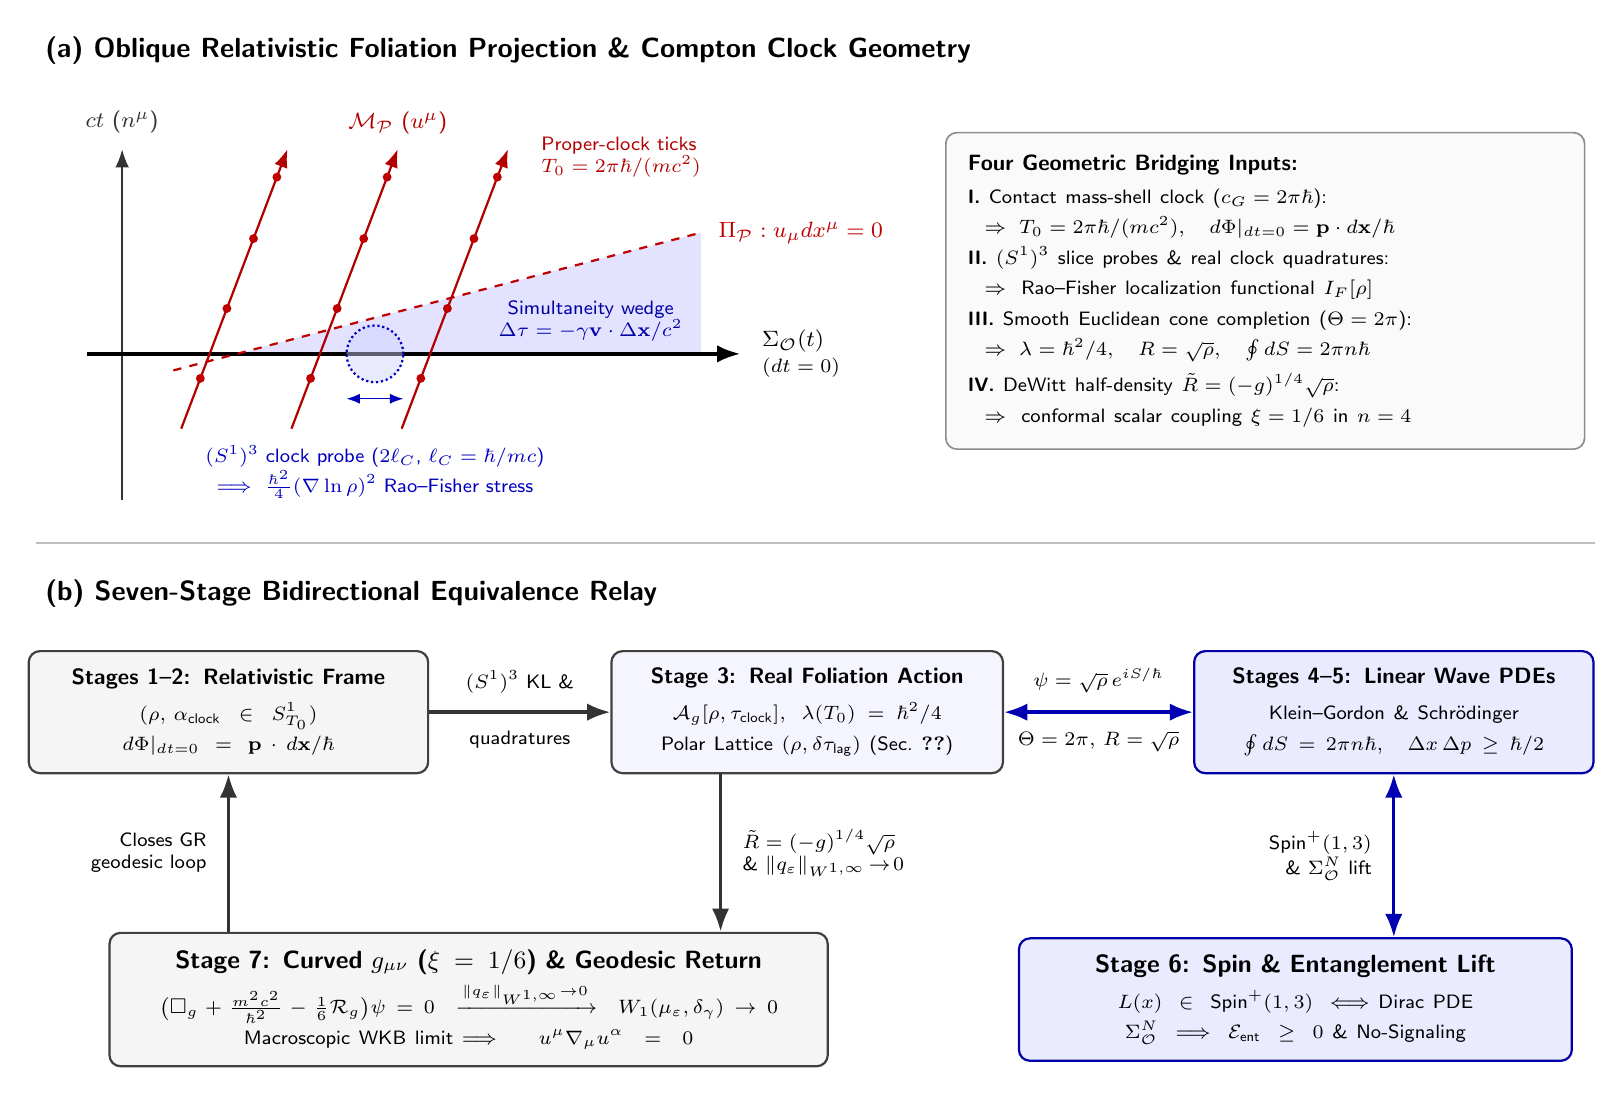
\begin{tikzpicture}[
    >=Latex,
    font=\sffamily\small,
    box/.style={draw=black!75, rounded corners=4pt, thick, align=center, inner sep=6pt, fill=blue!4},
    qbox/.style={draw=blue!65!black, rounded corners=4pt, thick, align=center, inner sep=6pt, fill=blue!8},
    rbox/.style={draw=black!75, rounded corners=4pt, thick, align=center, inner sep=6pt, fill=gray!8},
    notebox/.style={draw=black!45, rounded corners=4pt, semithick, align=left, inner sep=8pt, fill=gray!4},
    arr/.style={->, very thick, draw=black!80},
    biarr/.style={<->, very thick, draw=blue!70!black}
]
% ================ TOP PANEL (a): GEOMETRY OF INCOMPATIBLE FOLIATIONS ================
\node[anchor=north west, font=\sffamily\bfseries] at (0.0, 13.70) {(a) Oblique Relativistic Foliation Projection \& Compton Clock Geometry};

% Shaded simultaneity wedge between Sigma_O and Pi_P
\fill[blue!11] (2.55, 9.55) -- (8.45, 9.55) -- (8.45, 11.09) -- cycle;
\node[blue!65!black, font=\sffamily\scriptsize, align=center] at (7.05, 9.96) {Simultaneity wedge\\ $\Delta\tau = -\gamma\mathbf{v}\cdot\Delta\mathbf{x}/c^2$};

% Observer axes: ct and Sigma_O (dt = 0)
\draw[->, thick, black!80] (1.10, 7.70) -- (1.10, 12.15) node[above=2pt, font=\sffamily\footnotesize] {$ct$ ($n^\mu$)};
\draw[->, very thick, black] (0.65, 9.55) -- (8.95, 9.55) node[right=4pt, font=\sffamily\footnotesize, align=left] {$\Sigma_{\mathcal{O}}(t)$\\ {\scriptsize $(dt = 0)$}};

% Particle congruence worldlines u^mu (starting at y = 8.60 above lower label zone)
\foreach \xshift in {1.85, 3.25, 4.65} {
    \draw[->, thick, red!70!black] (\xshift, 8.60) -- ({\xshift + 1.35}, 12.15);
    \foreach \s in {0.18, 0.43, 0.68, 0.90} {
        \fill[red!75!black] ({\xshift + 1.35*\s}, {8.60 + 3.55*\s}) circle (1.6pt);
    }
}
\node[red!70!black, font=\sffamily\footnotesize, anchor=south] at (4.60, 12.22) {$\mathcal{M}_{\mathcal{P}}$ ($u^\mu$)};
\node[red!70!black, font=\sffamily\scriptsize, align=left, anchor=west] at (6.30, 12.05) {Proper-clock ticks\\ $T_0 = 2\pi\hbar/(mc^2)$};

% Tilted comoving rest hyperplane Pi_P: u_mu dx^mu = 0
\draw[thick, dashed, red!75!black] (1.75, 9.34) -- (8.45, 11.09);
\node[red!75!black, font=\sffamily\footnotesize, anchor=west] at (8.55, 11.09) {$\Pi_{\mathcal{P}}: u_\mu dx^\mu = 0$};

% Compton clock blur circle on Sigma_O (centered cleanly between worldlines 2 and 3)
\draw[thick, densely dotted, blue!75!black, fill=blue!18, fill opacity=0.45] (4.31, 9.55) circle (0.36);
\draw[<->, thin, blue!75!black] (3.95, 8.98) -- (4.67, 8.98);
\node[blue!75!black, font=\sffamily\scriptsize, align=center] at (4.31, 8.05) {$(S^1)^3$ clock probe ($2\ell_C$, $\ell_C = \hbar/mc$)\\ $\Longrightarrow\;\frac{\hbar^2}{4}(\nabla\ln\rho)^2$ Rao--Fisher stress};

% Right summary card in Panel (a) (wide enough that no item wraps onto an orphan line)
\node[notebox, anchor=west, text width=7.55cm] at (11.55, 10.35) {
    {\footnotesize\textbf{Four Geometric Bridging Inputs:}}\\[4pt]
    {\scriptsize \textbf{I.} Contact mass-shell clock ($c_G = 2\pi\hbar$):\\
    \hspace*{0.8em}$\Rightarrow\; T_0 = 2\pi\hbar/(mc^2),\quad d\Phi|_{dt=0} = \mathbf{p}\cdot d\mathbf{x}/\hbar$}\\[3pt]
    {\scriptsize \textbf{II.} $(S^1)^3$ slice probes \& real clock quadratures:\\
    \hspace*{0.8em}$\Rightarrow\;$ Rao--Fisher localization functional $I_F[\rho]$}\\[3pt]
    {\scriptsize \textbf{III.} Smooth Euclidean cone completion ($\Theta = 2\pi$):\\
    \hspace*{0.8em}$\Rightarrow\; \lambda = \hbar^2/4,\quad R = \sqrt{\rho},\quad \oint dS = 2\pi n\hbar$}\\[3pt]
    {\scriptsize \textbf{IV.} DeWitt half-density $\tilde{R} = (-g)^{1/4}\sqrt{\rho}$:\\
    \hspace*{0.8em}$\Rightarrow\;$ conformal scalar coupling $\xi = 1/6$ in $n = 4$}
};

% Horizontal divider between Panel (a) and Panel (b)
\draw[black!25, thick] (0.0, 7.15) -- (19.80, 7.15);

% ================ BOTTOM PANEL (b): BIDIRECTIONAL EQUIVALENCE RELAY ================
\node[anchor=north west, font=\sffamily\bfseries] at (0.0, 6.80) {(b) Seven-Stage Bidirectional Equivalence Relay};

% Top row of Panel (b): 3 boxes with explicit text width and 2.43 cm clear horizontal gaps
\node[rbox, text width=4.65cm, minimum height=1.55cm] (rel) at (2.45, 5.00) {
    {\footnotesize\textbf{Stages 1--2: Relativistic Frame}}\\[2pt]
    {\scriptsize $(\rho,\, \alpha_{\text{clock}} \in S^1_{T_0})$}\\
    {\scriptsize $d\Phi|_{dt=0} = \mathbf{p}\cdot d\mathbf{x}/\hbar$}
};

\node[box, text width=4.55cm, minimum height=1.55cm] (hjf) at (9.80, 5.00) {
    {\footnotesize\textbf{Stage 3: Real Foliation Action}}\\[2pt]
    {\scriptsize $\mathcal{A}_g[\rho,\tau_{\text{clock}}],\; \lambda(T_0)=\hbar^2/4$}\\
    {\scriptsize Polar Lattice $(\rho,\delta\tau_{\text{lag}})$ (Sec.~\ref{sec:numerical_simulations})}
};

\node[qbox, text width=4.65cm, minimum height=1.55cm] (qm) at (17.25, 5.00) {
    {\footnotesize\textbf{Stages 4--5: Linear Wave PDEs}}\\[2pt]
    {\scriptsize Klein--Gordon \& Schr\"{o}dinger}\\
    {\scriptsize $\oint dS = 2\pi n\hbar,\;\; \Delta x\,\Delta p \ge \hbar/2$}
};

% Bottom row of Panel (b): 2 wide boxes with 2.09 cm clear vertical gap below top row
\node[rbox, text width=8.70cm, minimum height=1.55cm] (gr) at (5.50, 1.35) {
    \textbf{Stage 7: Curved $g_{\mu\nu}$ ($\xi = 1/6$) \& Geodesic Return}\\[2pt]
    {\scriptsize $\big(\Box_g + \frac{m^2c^2}{\hbar^2} - \frac{1}{6}\mathcal{R}_g\big)\psi = 0 \;\xrightarrow{\|q_\varepsilon\|_{W^{1,\infty}}\to 0}\; W_1(\mu_\varepsilon,\delta_\gamma)\to 0$}\\
    {\scriptsize Macroscopic WKB limit $\Longrightarrow\; u^\mu\nabla_\mu u^\alpha = 0$}
};

\node[qbox, text width=6.60cm, minimum height=1.55cm] (ext) at (16.00, 1.35) {
    \textbf{Stage 6: Spin \& Entanglement Lift}\\[2pt]
    {\scriptsize $L(x)\in \text{Spin}^+(1,3) \Longleftrightarrow$ Dirac PDE}\\
    {\scriptsize $\Sigma_{\mathcal{O}}^N \Longrightarrow \mathcal{E}_{\text{ent}}\ge 0$ \& No-Signaling}
};

% Clean horizontal & vertical arrows in Panel (b) with named orthogonal coordinates
\draw[arr] (rel.east) -- node[above=3pt, font=\sffamily\scriptsize] {$(S^1)^3$ KL \&} node[below=3pt, font=\sffamily\scriptsize] {quadratures} (hjf.west);
\draw[biarr] (hjf.east) -- node[above=3pt, font=\sffamily\scriptsize] {$\psi=\sqrt{\rho}\,e^{iS/\hbar}$} node[below=3pt, font=\sffamily\scriptsize] {$\Theta=2\pi,\,R=\sqrt{\rho}$} (qm.west);
\draw[biarr] (qm.south) -- (qm.south |- ext.north) node[midway, left=4pt, font=\sffamily\scriptsize, align=right] {$\text{Spin}^+(1,3)$\\\& $\Sigma_{\mathcal{O}}^N$ lift};
\coordinate (hjfdrop) at ($(hjf.south)+(-1.10,0)$);
\draw[arr] (hjfdrop) -- (hjfdrop |- gr.north) node[midway, right=4pt, font=\sffamily\scriptsize, align=left] {$\tilde{R}=(-g)^{1/4}\sqrt{\rho}$\\\& $\|q_\varepsilon\|_{W^{1,\infty}}\!\to\! 0$};
\draw[arr] (gr.north -| rel.south) -- (rel.south) node[midway, left=4pt, font=\sffamily\scriptsize, align=right] {Closes GR\\geodesic loop};
\end{tikzpicture}%
}
\caption{Geometric mechanism and deductive relay of the relativistic foliation-incompatibility equivalence. \textbf{(a)} Any relative velocity $u^\mu \neq (c,\mathbf{0})$ tilts the comoving rest hyperplanes $\Pi_{\mathcal{P}}: u_\mu dx^\mu = 0$ across the observer's equal-time slice $\Sigma_{\mathcal{O}}(t)$ ($dt=0$), spanning the Lorentz simultaneity wedge $\Delta\tau = -\gamma\mathbf{v}\cdot\Delta\mathbf{x}/c^2$ across periodic proper-clock ticks $T_0 = 2\pi\hbar/(mc^2)$ while $(S^1)^3$ clock probes of Compton radius $\ell_C = \hbar/(mc)$ induce the spatial Rao--Fisher localization stress $\frac{\hbar^2}{4}(\nabla\ln\rho)^2$. \textbf{(b)} Seven-stage bidirectional relay linking real cross-foliation variables $(\rho, \tau_{\text{clock}})$ to linear scalar and spinorial quantum mechanics and returning in the macroscopic WKB limit ($\|q_\varepsilon\|_{W^{1,\infty}} \to 0$) to classical Einstein geodesics $u^\mu\nabla_\mu u^\alpha = 0$.}
\label{fig:foliation_bridge_schematic}
\end{figure}

\subsection{Relation to Earlier Geometric and Hydrodynamical Programs}
\label{sec:historical_synthesis}

Notably, the RFI--QM equivalence chain emerges quite straightforwardly by unifying two long-established geometric programs that developed largely in isolation, each supplying the piece missing from the other:

\begin{itemize}
    \item \textbf{Pillar I: The Relativistic Clock and Hydrodynamical Tradition (de Broglie 1924; Madelung 1927; Wigner 1939; Bohm 1952; Takabayasi 1952--1957; Hestenes 1966--1990; Greenberger 2001).} In his 1924 doctoral thesis \cite{deBroglie1924}, Louis de Broglie derived the phase of matter waves from the Lorentz relativity of simultaneity by modeling a massive particle as an internal clock of proper frequency $\omega_0 = mc^2/\hbar$---an insight sharpened by Greenberger \cite{Greenberger2001}, who showed that Galilean quantum phase transformations are residual proper-time slips of Lorentz simultaneity. Independently, Madelung \cite{Madelung1927} and Bohm \cite{Bohm1952} recast complex wave mechanics into real hydrodynamical continuity and Hamilton--Jacobi equations, while Wigner \cite{Wigner1939}, Takabayasi \cite{Takabayasi1952}, and Hestenes \cite{Hestenes1990} demonstrated that non-commuting Lorentz boosts and polar spinor decompositions encode Dirac spinor structure. \textit{Open question:} Pure relativistic clock models account for the quantum phase $S/\hbar$ and spin kinematics, but not for wavepacket dispersion or the Bohm quantum potential $Q$ without complex wave equations or added fluid stresses.
    \item \textbf{Pillar II: The Stochastic, Information-Geometry, and K\"{a}hler--Madelung Tradition (Stam 1959; Nelson 1966; Reginatto 1998--1999; Hall \& Reginatto 2002; Derakhshani 2015--2018; Khesin, Misio\l{}ek \& Modin 2018--2026; Caticha 2011--2019).} Stam \cite{Stam1959} showed that the mathematical form of the Heisenberg uncertainty principle is equivalent to the Cram\'{e}r--Rao inequality of statistical estimation. Nelson \cite{Nelson1966, Nelson2012} connected the osmotic velocity $\nabla\ln\rho$ to underlying sub-quantum Brownian diffusion, and Derakhshani \cite{Derakhshani2018} combined Nelsonian stochastic mechanics with a de Broglie--Hestenes \textit{zitterbewegung} internal clock to address Wallstrom's circulation critique within a stochastic ether model. From the deterministic variational side, Reginatto \cite{Reginatto1998, Reginatto1999}, Hall and Reginatto \cite{HallReginatto2002}, and Caticha \cite{Caticha2019} showed that endowing probability density space with the Rao--Fisher metric $I_F[\rho]$ linearizes Hamilton--Jacobi--Fisher dynamics under $\psi = \sqrt{\rho}e^{iS/\hbar}$, while Khesin, Misio\l{}ek, and Modin \cite{Khesin2018, Khesin2026} established the infinite-dimensional K\"{a}hler--Poisson geometry and nodal-vortex structure of the Madelung transform. \textit{Open question:} Without a relativistic cross-foliation clock mechanism, stochastic approaches must postulate a sub-quantum diffusion process that resists Lorentz-covariant extension \cite{Gaveau1984}, whereas purely information-theoretic or non-relativistic K\"{a}hler approaches leave open why quantum congruences experience Fisher dispersion stress with coupling $\lambda = \hbar^2/4$ while classical statistical ensembles do not.
\end{itemize}

\begin{table}[htbp]
\centering
\caption{Synthesis of Foundational Approaches to Emergent Quantum Mechanics}
\label{tab:synthesis}
\vspace{0.5em}
\footnotesize
\setlength{\tabcolsep}{4pt}
\begin{tabularx}{\textwidth}{>{\raggedright\arraybackslash}p{0.23\textwidth} >{\raggedright\arraybackslash}X >{\raggedright\arraybackslash}X >{\raggedright\arraybackslash}X}
\toprule
\textbf{Framework} & \textbf{Origin of Phase $\Phi = S/\hbar$} & \textbf{Origin of Amplitude $\sqrt{\rho}$ \& Quantum Potential} & \textbf{Status of Global Equivalence} \\
\midrule
\textbf{Relativistic Clock / Hydrodynamics} (de Broglie, Madelung, Bohm, Hestenes) & Lorentz simultaneity tilt between $\Sigma_{\mathcal{P}}$ and $\Sigma_{\mathcal{O}}$ & Postulated from $\psi$ or inserted via pilot-wave fluid stresses & Incomplete: lacks clock construction of Fisher potential $Q$ \\
\addlinespace
\textbf{Stochastic / Zitterbewegung Mechanics} (Nelson \cite{Nelson1966}, Derakhshani \cite{Derakhshani2018}) & Osmotic/current drift velocity potential or \textit{zitterbewegung} clock & Sub-quantum Brownian diffusion with postulated diffusivity $\hbar/(2m)$ & Non-covariant Markovian diffusion \cite{Gaveau1984}; requires stochastic ether \\
\addlinespace
\textbf{Fisher / K\"{a}hler Hydrodynamics} (Reginatto, Hall, Caticha; Khesin \& Modin \cite{Khesin2018, Khesin2026}) & Hamilton--Jacobi multiplier or K\"{a}hler symplectic conjugate & Rao--Fisher metric $I_F[\rho]$ flattened via $R = \sqrt{\rho}$ & Wallstrom $\oint dS = 2\pi n\hbar$ imposed or analyzed non-relativistically \\
\addlinespace
\textbf{Quantum Reference Frames} (Brukner, Giacomini \cite{Giacomini2019}) & Assumed via standard Hilbert space axioms & Frame-dependent superposition under quantum coordinate maps & Assumes Hilbert space formalism a priori \\
\addlinespace
\textbf{Present Work} (Foliation Incompatibility) & Phase-clock 1-form $\alpha_{\text{clock}} = -dS/(mc^2)$ ($= \beta_{\text{proper}}$ on $\mathcal{H}_m$) & $(S^1)^3$ clock KL Hessian, real clock quadratures, \& smooth cone completion ($\Theta = 2\pi \Rightarrow \lambda = \hbar^2/4, R = \sqrt{\rho}$) & Deterministic Lorentzian $U(1)$-quotient bijection via $S^1_{T_0}$ holonomy \& codimension-2 PDE removability (Theorems \ref{thm:clock_sideband}--\ref{thm:wallstrom}) \\
\bottomrule
\end{tabularx}
\end{table}

As summarized in Table~\ref{tab:synthesis}, coupling these two programs closes both gaps simultaneously. First, the contrast between quantum congruences and classical statistical ensembles reduces to the presence or absence of the $S^1_{T_0}$ clock fiber: phase-averaging a $T_0$-periodic clock and requiring smooth Euclidean cone completion at nodal zeros ($\Theta = 2\pi$) locks $\lambda = \hbar^2/4$ directly to $T_0$ without any stochastic diffusion postulate, while sending $T_0, \ell_C \to 0$ ($\hbar \to 0$ at fixed $m, c$) recovers classical non-dispersive dust (Theorem~\ref{thm:clock_sideband} and Lemma~\ref{lem:uniqueness}). Second, Wallstrom's objection \cite{Wallstrom1994, Schmelzer2011} dissolves because the global phase variable is a circle-valued section $q: \mathcal{M}\setminus\mathcal{N} \to S^1_{T_0}$ rather than a globally single-valued real function $S$: its closed 1-form $\alpha_{\text{clock}} = d\tau_{\text{clock}} = -dS/(mc^2)$ naturally carries integer Sagnac holonomy $\oint_C \alpha_{\text{clock}} = -n T_0 \iff \oint_C dS = 2\pi n\hbar$, and codimension-2 PDE removability extends $\psi = Rq$ smoothly across the nodal set $\mathcal{N}$ (Theorem~\ref{thm:wallstrom}).

Thus, none of the individual mathematical tools presented here required inventing exotic differential operators. Each draws on established machinery from contact geometry \cite{Gromov1985}, information geometry and K\"{a}hler hydrodynamics \cite{Stam1959, Cencov1982, Reginatto1999, HallReginatto2002, Khesin2018, Khesin2026}, hyperbolic wave regularity \cite{BarGinouxPfaffle2007, Bar2015}, Clifford spinor decompositions \cite{Takabayasi1952, Hestenes1990}, and curved-spacetime half-densities \cite{DeWitt1957}. What was missing was merely the observation that projecting an oblique relativistic congruence $\mathcal{M}_{\mathcal{P}}$ onto an observer foliation $\mathcal{M}_{\mathcal{O}}$ locks these separate structures together as consecutive links of a single geometric chain.

%======================================================================
\section{\texorpdfstring{Numerical Experiments in Purely Real Foliation Variables}{Numerical Experiments in Purely Real Foliation Variables}}
\label{sec:numerical_simulations}
%======================================================================

Because the RFI--QM equivalence is constructive from end to end, it offers an unusually direct computational test of the analytical framework. Rather than taking complex Hilbert-space evolution for granted, we can discard complex arithmetic altogether, supply purely real cross-foliation data---spatial density $\rho$ and relativistic clock lag $\delta\tau_{\text{lag}}$---to a real-variable kernel, and test whether hallmark quantum phenomena emerge where matched classical ensembles fail. Before turning to the formal proofs in Sections~\ref{sec:setup}--\ref{sec:curved_spacetime}, we carry out this test across four progressively stronger benchmarks: free wavepacket dispersion from rest, Young double-slit interference across deep zero-density nodes, sub-barrier tunneling with quantized vortex nucleation, and finite-$c$ relativistic Klein--Gordon dispersion.

\subsection{\texorpdfstring{The Geometric-Mean Polar Lattice on $\mathbb{R}^+ \times S^1_{T_0}$}{The Geometric-Mean Polar Lattice on R+ x S1}}
\label{sec:polar_lattice}

Let $\delta\tau_{\text{lag}}(x, t) \equiv t - \tau_{\text{clock}}(x, t) = +\tilde{S}(x, t)/(mc^2) \in S^1_{T_0} = \mathbb{R}/T_0\mathbb{Z}$ denote the reduced phase-clock lag in the small-boost regime of Corollary~\ref{cor:schrodinger}, and let $\ell_C \equiv \hbar/(mc)$ denote the reduced Compton length ($T_0 = 2\pi\ell_C / c$). Dividing the frame-mismatch PDEs by $mc^2$ expresses the continuum dynamics solely in terms of $(c, \ell_C)$:
\begin{align}
\frac{\partial \rho}{\partial t} + \frac{\partial}{\partial x}\left( \rho \, v_{\text{rel}} \right) &= 0, \qquad v_{\text{rel}}(x, t) \equiv c^2 \frac{\partial (\delta\tau_{\text{lag}})}{\partial x}, \label{eq:real_pde_continuity} \\
\frac{\partial (\delta\tau_{\text{lag}})}{\partial t} &= -\frac{1}{2} c^2 \left( \frac{\partial (\delta\tau_{\text{lag}})}{\partial x} \right)^2 - \frac{V(x)}{m c^2} + \frac{\ell_C^2}{2} \frac{\partial_x^2 \sqrt{\rho}}{\sqrt{\rho}}. \label{eq:real_pde_clock}
\end{align}

Consider a uniform spatial grid $x_j = j\Delta x$ with dimensionless link clock difference $\Delta\phi_{j+1/2} \equiv \frac{c}{\ell_C}(\delta\tau_{j+1} - \delta\tau_j) \in \mathbb{R}/2\pi\mathbb{Z}$ and signed real amplitude $R_j$. By Theorem~\ref{thm:wallstrom}, $\delta\tau_j$ lives on the compact circle $S^1_{T_0}$ rather than $\mathbb{R}$, avoiding $O(T_0/\Delta x)$ branch-cut jumps across Sagnac vortices ($\oint d\delta\tau_{\text{lag}} = \pm T_0$). Comparing the two natural real discretizations of the ADM energy on $\mathbb{R}^+ \times S^1_{T_0}$ exposes the exact source of the node stiffness that has historically plagued hydrodynamic quantum solvers:
\begin{enumerate}[label=(\alph*)]
    \item \textbf{Geometric-mean polar K\"{a}hler lattice:} Coupling adjacent sites via the geometric mean $R_{j+1} R_j$ defines the real polar Hamiltonian
    \begin{equation}
    \label{eq:polar_kahler_lattice}
    \begin{aligned}
    \mathcal{H}_{\Delta x}^{\text{polar}}[R, \delta\tau_{\text{lag}}] = \sum_j \Delta x \Bigg\{ &R_{j+1} R_j \frac{\ell_C^2}{\Delta x^2}\left[ 1 - \cos(\Delta\phi_{j+1/2}) \right] \\
    &\quad + \frac{\ell_C^2}{2}\left( \frac{R_{j+1} - R_j}{\Delta x} \right)^2 + R_j^2 \frac{V_j}{m c^2} \Bigg\}.
    \end{aligned}
    \end{equation}
    Varying $\mathcal{H}_{\Delta x}^{\text{polar}}$ gives purely real evolution equations (with odd-parity-preserving node regularization $1/R_j \mapsto \frac{R_j}{R_j^2 + \varepsilon_{\text{reg}}^2}$, $\varepsilon_{\text{reg}} \in [10^{-10}, 10^{-6}]$):
    \begin{align}
    \frac{dR_j}{dt} &= -\frac{\ell_C c}{2\Delta x^2}\Big[ R_{j+1}\sin(\Delta\phi_{j+1/2}) - R_{j-1}\sin(\Delta\phi_{j-1/2}) \Big], \label{eq:polar_dR_dt} \\
    \frac{d(\delta\tau_j)}{dt} &= \frac{R_j}{R_j^2 + \varepsilon_{\text{reg}}^2}\frac{\ell_C^2}{2\Delta x^2}\Big\{ (R_{j+1} - 2R_j + R_{j-1}) - R_{j+1}\big[1 - \cos(\Delta\phi_{j+1/2})\big] \nonumber \\
    &\qquad\qquad\qquad\qquad\quad - R_{j-1}\big[1 - \cos(\Delta\phi_{j-1/2})\big] \Big\} - \frac{V_j}{mc^2}, \label{eq:polar_dtau_dt}
    \end{align}
    together with the strictly non-negative density $\rho_j = R_j^2 \ge 0$, zero artificial clock viscosity ($\nu_{\text{clock}} = 0$), and regularized link drift velocity
    \begin{equation}
    \label{eq:s1_staggered_velocity}
    \begin{aligned}
    v_j &= \frac{J_{j+1/2} + J_{j-1/2}}{2\left(\rho_j + \varepsilon_{\text{reg}}^2\right)}, \\
    J_{j+1/2} &\equiv R_j R_{j+1}\frac{\ell_C c}{\Delta x}\sin(\Delta\phi_{j+1/2}) = \rho\,c^2 \frac{\partial(\delta\tau_{\text{lag}})}{\partial x} + O(\Delta x^2),
    \end{aligned}
    \end{equation}
    which is second-order accurate at interior sites (with $O(\Delta x)$ Neumann boundary truncation at replicated endpoints unless $\partial_x\delta\tau_{\text{lag}} = 0$). By the law of cosines, $R_{j+1}R_j[1 - \cos(\Delta\phi_{j+1/2})] + \frac{1}{2}(R_{j+1} - R_j)^2 = \frac{1}{2}|\Psi_{j+1} - \Psi_j|^2$. Eqs.~\eqref{eq:polar_dR_dt}--\eqref{eq:polar_dtau_dt} are therefore the exact real polar counterpart of the discrete Schr\"{o}dinger system (Theorem~\ref{thm:kahler}): for $\varepsilon_{\text{reg}} = 0$ on $R_j \neq 0$, $\mathcal{H}_{\Delta x}^{\text{polar}}$ is conserved identically, while $\varepsilon_{\text{reg}} > 0$ introduces only a localized $O\big(\varepsilon_{\text{reg}}^2 / (R_j^2 + \varepsilon_{\text{reg}}^2)\big)$ residual at nodal cores. Whenever $R_j(t)$ changes sign across a nodal curve, we canonicalize the positive-amplitude state via $\rho_j = R_j^2$ and $\delta\tau_{\text{canon}, j} = \delta\tau_j + \frac{T_0}{2}\mathbf{1}_{R_j < 0} \pmod{T_0}$.
    \item \textbf{Arithmetic-mean hydrodynamic lattice:} Replacing $R_{j+1}R_j$ by the arithmetic mean $\frac{1}{2}(\rho_{j+1} + \rho_j)$ yields the staggered hydrodynamic Hamiltonian
    \begin{equation}
    \label{eq:s1_lattice_hamiltonian}
    \begin{aligned}
    \mathcal{H}_{\Delta x}^{\text{arith}}[\rho, \delta\tau_{\text{lag}}] = \sum_j \Delta x \Bigg\{ &\frac{\rho_{j+1} + \rho_j}{2} \frac{\ell_C^2}{\Delta x^2}\left[ 1 - \cos(\Delta\phi_{j+1/2}) \right] \\
    &\quad + \frac{\ell_C^2}{2}\left( \frac{R_{j+1} - R_j}{\Delta x} \right)^2 + \rho_j \frac{V_j}{m c^2} \Bigg\}.
    \end{aligned}
    \end{equation}
    Because $\frac{1}{2}(\rho_{j+1} + \rho_j) - R_{j+1}R_j = \frac{1}{2}(R_{j+1} - R_j)^2$, Eq.~\eqref{eq:s1_lattice_hamiltonian} departs from the exact K\"{a}hler lattice \eqref{eq:polar_kahler_lattice} by an $O\big((\Delta R)^2[1 - \cos\Delta\phi]\big)$ defect concentrated precisely at deep interference nodes ($\rho_j \to 0, \Delta\phi \approx \pi$). That algebraic discrepancy mirrors the node stiffness of traditional hydrodynamic quantum-trajectory schemes \cite{Lopreore1999}; switching to the geometric-mean link \eqref{eq:polar_kahler_lattice} removes both the outer-lobe phase-wall artifact and any need for artificial viscosity.
\end{enumerate}

\subsection{Free Dispersion, Double-Slit Interference, and Sub-Barrier Tunneling}
\label{sec:subluminal_benchmarks}

We integrated Eqs.~\eqref{eq:polar_dR_dt}--\eqref{eq:polar_dtau_dt} using classical fourth-order Runge--Kutta (RK4) in units $\hbar = m = 1$ with $c = 20$ and $\ell_C = 1/c = 0.05$, placing all initial wavepackets in the subluminal, multi-Compton regime ($\Delta x \in [11\ell_C, 40\ell_C], |v_0| \ll c$). To test genuine wave behavior rather than cold-ray kinematics ($\ell_C = 0$), we benchmarked the real polar $(R, \delta\tau_{\text{lag}})$ solver not only against spectral Fourier Schr\"{o}dinger evolution and the same-lattice unitary matrix exponential $e^{-i H_{\Delta x} t}\Psi(0)$, but also against matched classical Liouville/Wigner ensembles sharing the exact initial spatial density $\rho_0(x)$ and minimum-uncertainty momentum width $\sigma_p = \hbar/(2\sigma_x)$ (Table~\ref{tab:sim_benchmarks} and Figure~\ref{fig:foliation_showcase}).

\begin{enumerate}[label=\textbf{Experiment \arabic*:}, leftmargin=2.5cm]
    \item \textbf{Free Gaussian dispersion.} We initialized a Gaussian density $\rho_0(x) = (2\pi\sigma_0^2)^{-1/2}e^{-x^2/(2\sigma_0^2)}$ ($\sigma_0 = 1.0 = 20\ell_C$) with completely flat clock synchronization $\delta\tau_{\text{lag}}(x,0) = 0$ ($v_{\text{rel}} = 0$ everywhere) and evolved to $T = 3.0$. A cold classical dust cloud remains static ($\sigma_{\text{dust}} = 1.000000$), whereas a classical Wigner ensemble ($N = 4 \times 10^5$ trajectories with $\sigma_p = 1/(2\sigma_0)$) spreads to $\sigma_{\text{Wigner}} = 1.799947$, matching the exact quantum width $\sigma_{\text{QM}} = \sigma_0\sqrt{1 + (T/2\sigma_0^2)^2} = 1.802776$. Starting from zero initial velocity variance, the real polar solver spreads to $\sigma_{\text{sim}} = 1.802240$ (relative error $2.97 \times 10^{-4}$, $L^1$ density error $2.0 \times 10^{-4}$, $\max|v_{\text{rel}}|/c = 0.068$). The Fisher clock-dilation term $+\frac{1}{2}\ell_C^2(\partial_x^2 R)/R$ dynamically converts the initial spatial localization $I_F[\rho_0]$ (Theorems~\ref{thm:clock_sideband} and~\ref{thm:uncertainty}) into bulk simultaneity tilt.

    \item \textbf{Young double-slit interference.} We next initialized the coherent two-slit modulus $\rho_0(x) = Z_0^{-1}\big[e^{-(x + d/2)^2/(2w^2)} + e^{-(x - d/2)^2/(2w^2)}\big]$ ($d = 4.0$, $w = 0.55 = 11\ell_C$, $\delta\tau_{\text{lag}}(x,0) = 0$, normalized by $Z_0$) and evolved to $T = 3.2$. Here the matched incoherent two-slit Wigner mixture fails qualitatively, collapsing into a single broad central hump ($\rho_{\text{Wigner}}(0, T) = 0.1073$, zero fringes). With zero artificial viscosity, the real polar solver reproduces the full multi-fringe Young interference pattern across deep $\rho \to 0$ nodes, reaching a central peak $\rho_{\text{sim}}(0, T) = 0.2130$ against Fourier QM's $0.2129$ (relative error $7.76 \times 10^{-4}$, global $L^1 = 9.0 \times 10^{-4}$, three prominent peaks $>5\%$ of maximum on $[-9, 9]$, $\max|v_{\text{rel}}|/c = 0.137$). Non-crossing of the 1D integral curves $dx_k/dt = v_{\text{rel}}(x_k, t)$ across $x = 0$ follows automatically from ODE uniqueness and mirror symmetry $v_{\text{rel}}(0, t) = 0$.

    \item \textbf{Sub-barrier quantum tunneling and vortex nucleation.} Finally, we launched a boosted Gaussian packet ($x_0 = -6.5$, $\sigma_0 = 2.0 = 40\ell_C$, $v_0 = 2.0 = 0.10c$, mean kinetic energy $K_0 = 2.0$) against a repulsive Gaussian barrier $V(x) = V_0\exp[-x^2/(2w_b^2)]$ of height $V_0 = 1.42 K_0 = 2.84$ and width $w_b = 0.45$. Because $\sigma_p = 1/(2\sigma_0) = 0.25$, only $6.26\%$ of the initial Wigner kinetic-energy distribution exceeds $V_0$ ($6.23\%$ in a $10^6$-draw Monte Carlo sample). At the active collision snapshot $T = 4.2$, the classical Wigner ensemble transmits just $4.05\%$ beyond $x = 1.5$ (cold ray: $0.00\%$), whereas both Fourier QM ($16.48\%$) and the real polar solver ($16.35\%$, relative error $8.10 \times 10^{-3}$, global $L^1 = 0.0046$, reflected-side $L^1 = 0.0015$) achieve a $4.07\times$ quantum tunneling excess while nucleating the exact same spacetime Sagnac vortex count ($4+/0-$). Integrating to the post-collision asymptotic regime $T_{\text{asymp}} = 9.0$ (residual barrier probability $3.8 \times 10^{-4}$), both the real polar solver and Fourier QM transmit $30.3\%$ versus $6.5\%$ for the Wigner baseline---a $4.7\times$ excess. This agrees with the stationary two-point Numerov scattering transmission ($30.12\%$); the slight $0.2\%$ offset reflects finite initial tail overlap with $V(x)$ at $x_0 = -6.5$ ($\langle V \rangle_0 \approx 4.1 \times 10^{-3}$), and initializing at $x_0 = -12$ converges directly to $30.12\%$. Near deep reflected standing-wave nodes ($\rho \to 0$), the non-relativistic current-to-density drift locally reaches $\max|v_{\text{rel}}|/c = 1.549$, anticipating the sub-Compton spacelike phase regime $(\partial S)^2 < 0$ analyzed in Theorem~\ref{thm:wallstrom} and Remark~\ref{rem:subcompton_spinor_bridge}.
\end{enumerate}

\paragraph{Discretization and same-lattice verification.}
To separate finite-difference discretization error from the real polar reformulation itself, we compared the reconstructed field $\Psi_j = \sqrt{\rho_j}e^{i(c/\ell_C)\delta\tau_{\text{canon}, j}}$ directly against the same-lattice unitary matrix exponential $e^{-i H_{\Delta x} t}\Psi(0)$ using the trapezoid-normalized, global-phase-aligned ray distance $L^2_{\text{FD}}$. Across all runs, agreement reaches $5.44 \times 10^{-10}$ in Experiment~1 ($x \in [-15, 15)$, $N_x = 512$, $600 \times 12$ RK4 steps, $\varepsilon_{\text{reg}} = 10^{-10}$), $4.90 \times 10^{-8}$ in Experiment~2 ($x \in [-18, 18]$, $N_x = 1025$, $1600 \times 18$ steps, $\varepsilon_{\text{reg}} = 10^{-9}$), $1.87 \times 10^{-5}$ in Experiment~3 at $T = 4.2$ ($x \in [-28, 28)$, $N_x = 1024$, $1800 \times 18$ steps, $\varepsilon_{\text{reg}} = 10^{-6}$), and $3.85 \times 10^{-5}$ at $T_{\text{asymp}} = 9.0$ ($x \in [-56, 56)$, $N_x = 2048$, $900 \times 18$ steps). Saved-time relative peak-to-peak drift $(\max A - \min A)/|A(0)|$ stays below $5.22 \times 10^{-15}$ for discrete norm ($3.18 \times 10^{-12}$ at $T = 9.0$) and below $7.60 \times 10^{-9}$ for discrete energy ($2.36 \times 10^{-8}$ at $T = 9.0$, due solely to $\varepsilon_{\text{reg}} > 0$ and RK4 time-stepping). Virtually all of the $2.6 \times 10^{-4}$ to $3.9 \times 10^{-3}$ difference relative to spectral split-step Fourier QM therefore comes from comparing finite-difference and spectral Laplacians.

\begin{table}[htbp]
\centering
\caption{Benchmark Comparison ($\hbar = m = 1$; $c = 20, \ell_C = 0.05$ in Experiments 1--3) of Classical Wigner Baselines, Real Polar $(R, \delta\tau_{\text{lag}})$ K\"{a}hler Lattice Solver, Same-Lattice Matrix Exponential (ray $L^2_{\text{FD}}$), Spectral Fourier Schr\"{o}dinger Evolution (ray $L^2_{\text{FFT}}$), and Relativistic Klein--Gordon Dispersion (Experiment 4)}
\label{tab:sim_benchmarks}
\vspace{0.5em}
\footnotesize
\setlength{\tabcolsep}{4pt}
\begin{tabularx}{\textwidth}{>{\raggedright\arraybackslash}p{0.20\textwidth} >{\raggedright\arraybackslash}p{0.15\textwidth} >{\raggedright\arraybackslash}p{0.14\textwidth} >{\raggedright\arraybackslash}p{0.13\textwidth} >{\raggedright\arraybackslash}X}
\toprule
\textbf{Experiment \& Observable} & \textbf{Classical Wigner Baseline (same $\rho_0$)} & \textbf{Real Polar $(R, \delta\tau)$ Solver} & \textbf{Fourier QM} & \textbf{Same-Lattice ray $L^2_{\text{FD}}$, $L^1(\rho)$, \& Spectral $L^2_{\text{FFT}}$} \\
\midrule
\textbf{1. Free Dispersion} $\sigma(T = 3.0)$ & $1.799947$ (cold dust: $1.000$) & $\mathbf{1.802240}$ & $1.802776$ & ray $L^2_{\text{FD}} = 5.44 \times 10^{-10}$ ($L^1 = 0.0002$, $L^2_{\text{FFT}} = 2.6 \times 10^{-4}$) \\
\addlinespace
\textbf{2. Double-Slit} $\rho(0, T = 3.2)$ & $0.1073$ ($1$ hump, $0$ fringes) & $\mathbf{0.2130}$ ($3$ peaks) & $0.2129$ ($3$ peaks) & ray $L^2_{\text{FD}} = 4.90 \times 10^{-8}$ ($L^1 = 0.0009$, $L^2_{\text{FFT}} = 1.3\times 10^{-3}$) \\
\addlinespace
\textbf{3. Sub-Barrier Tunneling} $P(x > 1.5, T = 4.2)$ & $0.0405$ (cold ray: $0.0000$) & $\mathbf{0.1635}$ (nodes: $4+/0-$) & $\mathbf{0.1648}$ (nodes: $4+/0-$) & ray $L^2_{\text{FD}} = 1.87 \times 10^{-5}$ ($L^1 = 0.0046$, $L^2_{\text{FFT}} = 3.9\times 10^{-3}$; $T=9$: $30.3\%$ vs.\ $6.5\%$, $4.7\times$) \\
\midrule
\multicolumn{5}{@{}p{\textwidth}@{}}{\textit{Relativistic Real-Quadrature Klein--Gordon Dispersion Scan ($x \in [-25, 25),\, N_x = 2048,\, v_0 = 1.5,\, T = 3.0$; Sec.~\ref{sec:kg_dispersion}):}} \\
\textbf{4. Boosted KG Width} $\sigma_{|\psi|^2}(T=3.0)$ & --- & \multicolumn{2}{>{\raggedright\arraybackslash}p{0.27\textwidth}}{$c = 2$ ($v_0 = 0.75c$): $\mathbf{1.1097}$\newline $c = 20$ ($v_0 = 0.075c$): $1.7912$} & Longitudinal $\gamma^{-3}$ Lorentz inertia suppression of spreading \\
\bottomrule
\end{tabularx}
\end{table}

\begin{figure}[htbp]
\centering
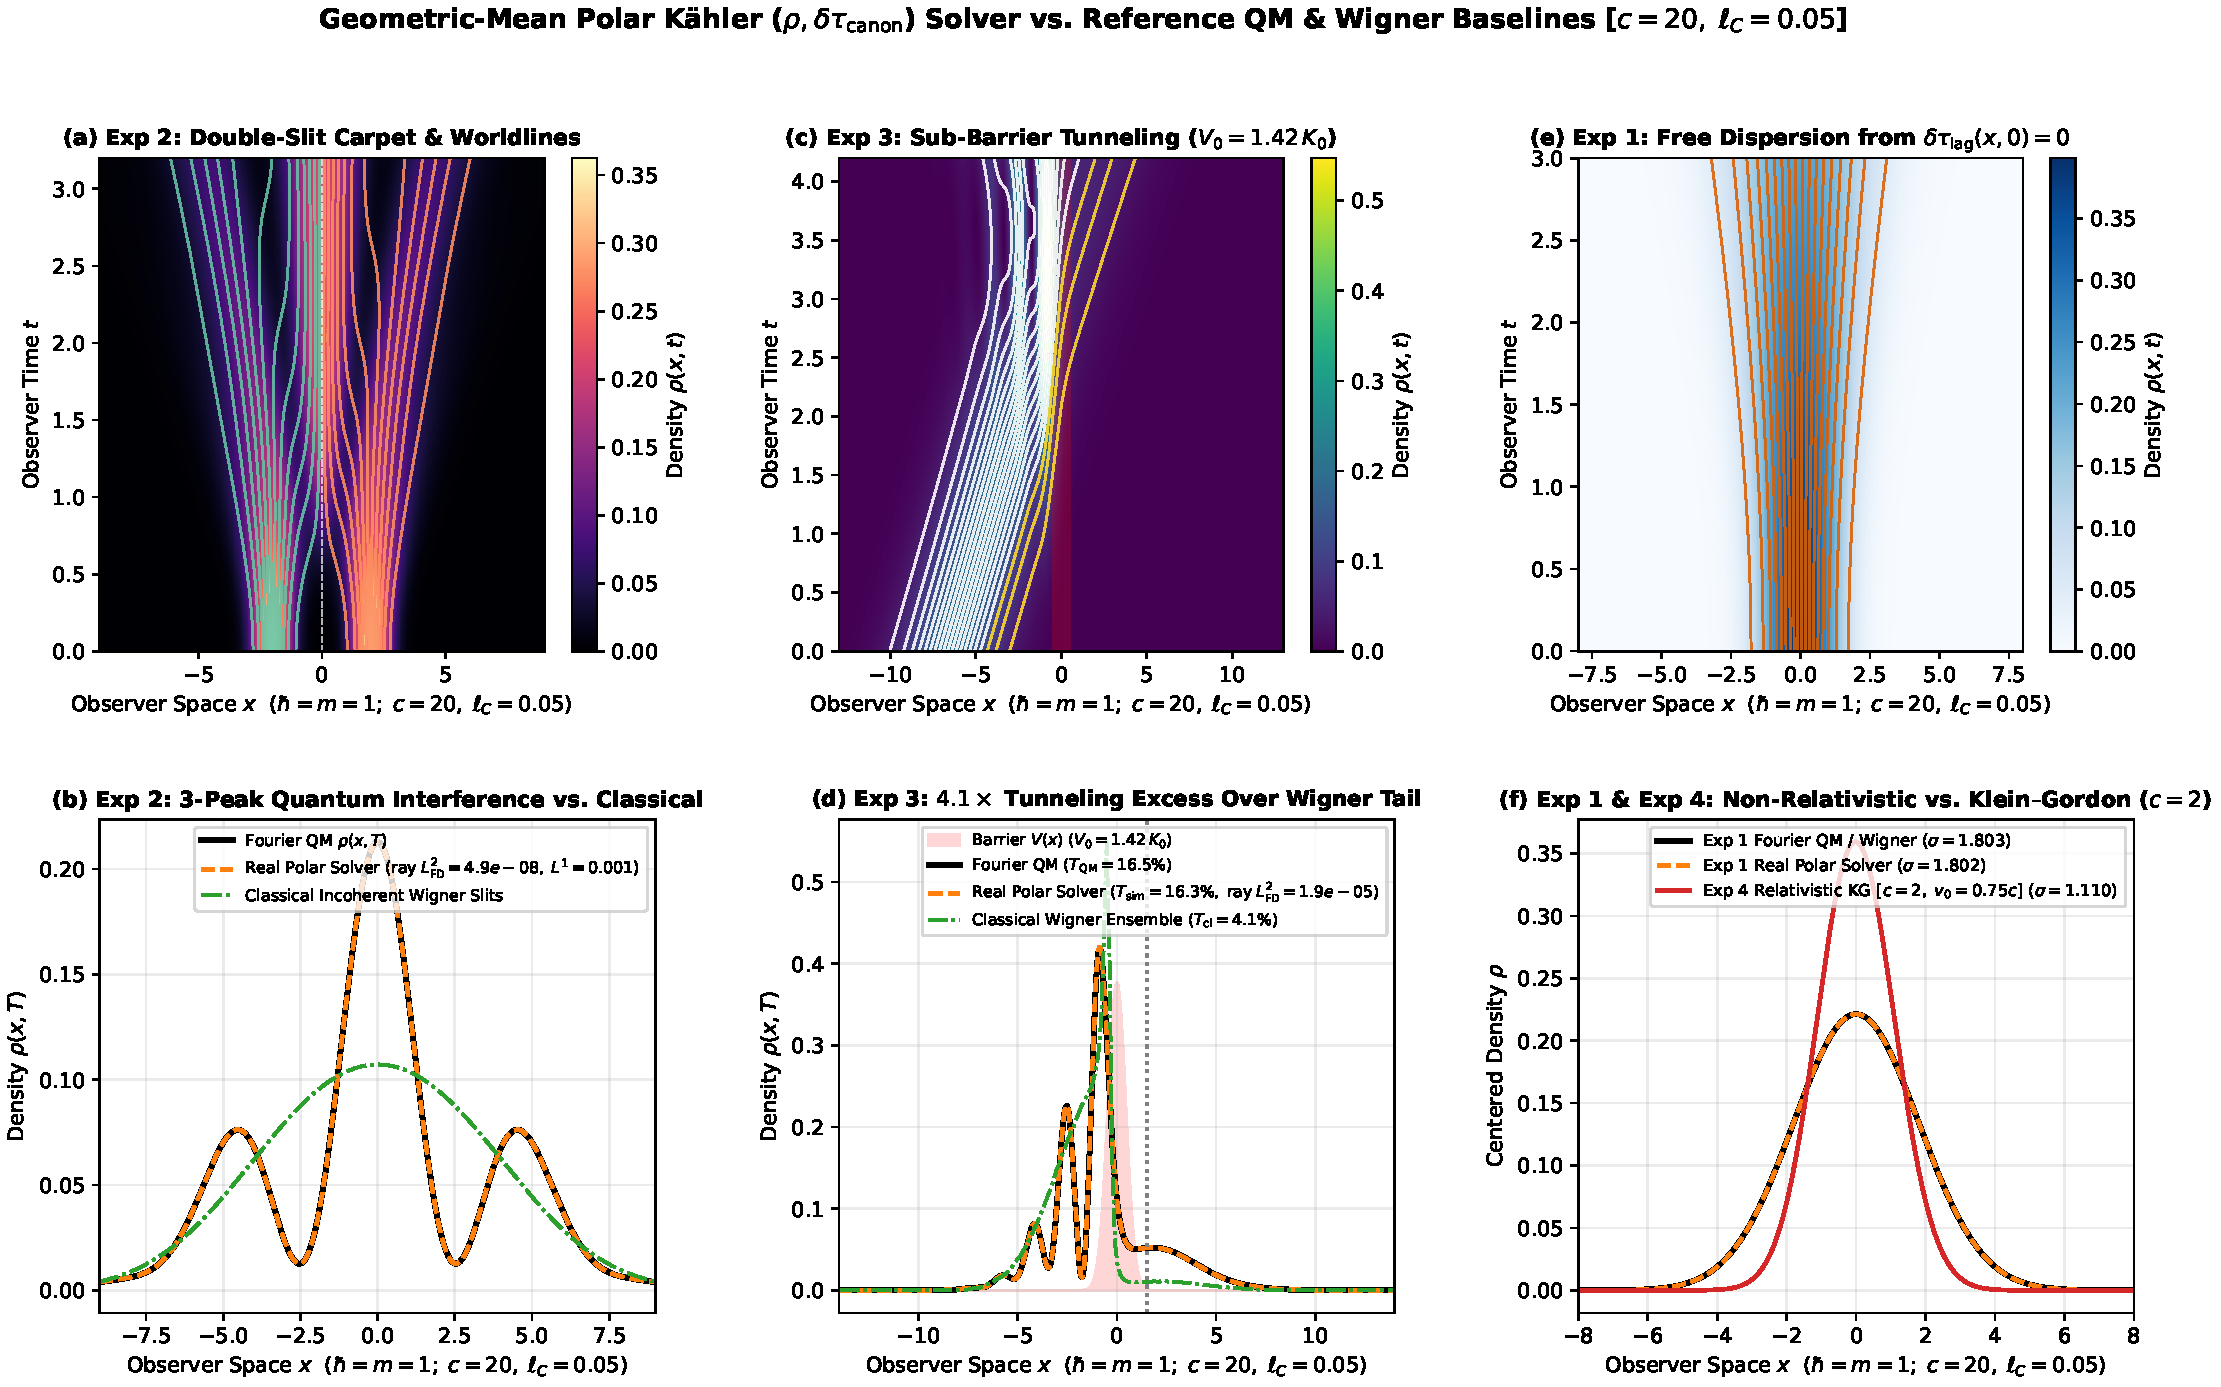
\includegraphics[width=\textwidth]{showcase_v9.pdf}
\caption{Real-variable polar K\"{a}hler benchmarks versus reference quantum and classical Wigner baselines ($c = 20, \ell_C = 0.05, \hbar = m = 1$). \textbf{(a, b)} Experiment~2 (double-slit): the incoherent Wigner mixture produces a single smooth hump ($0.1073$), whereas the zero-viscosity real polar solver reproduces the multi-fringe interference pattern ($L^2_{\text{FD}} = 4.90 \times 10^{-8}$, $L^1 = 0.0009$). \textbf{(c, d)} Experiment~3 (sub-barrier tunneling, $V_0 = 1.42 K_0$): at $T = 4.2$, the real polar solver ($16.35\%$) and Fourier QM ($16.48\%$) achieve a $4.1\times$ excess over the classical Wigner tail ($4.05\%$) with identical $4+/0-$ Sagnac vortex counts ($30.3\%$ vs.\ $6.5\%$, or $4.7\times$, at $T_{\text{asymp}} = 9.0$). \textbf{(e, f)} Experiment~1 (free dispersion from $\delta\tau_{\text{lag}}(x,0) = 0$, $L^2_{\text{FD}} = 5.44 \times 10^{-10}$) alongside Experiment~4 (normalized modulus density $|\psi|^2$ under relativistic Klein--Gordon dispersion at $c = 2, v_0 = 0.75c$, showing longitudinal $\gamma^{-3}$ suppression $\sigma = 1.110$ vs.\ $1.791$ at $c = 20$).}
\label{fig:foliation_showcase}
\end{figure}

\subsection{\texorpdfstring{Relativistic Klein--Gordon Dispersion and the Role of $c$}{Relativistic Klein-Gordon Dispersion and the Role of c}}
\label{sec:kg_dispersion}

A sharp diagnostic separates the non-relativistic parabolic reduction \eqref{eq:real_pde_continuity}--\eqref{eq:real_pde_clock} from the full relativistic Klein--Gordon foliation system of Theorems~\ref{thm:kahler} and~\ref{thm:adm_positivity}. Writing $\tilde{S} = mc^2 \delta\tau_{\text{lag}}$ in Eqs.~\eqref{eq:real_pde_continuity}--\eqref{eq:real_pde_clock} shows that $c$ and $\ell_C = \hbar/(mc)$ enter only through the Galilean product $c\ell_C = \hbar/m$; integrating Experiment~1 at $c = 1$ ($\ell_C = 1$) and $c = 20$ ($\ell_C = 0.05$) indeed yields identical density histories to floating-point roundoff ($\max_{x,t} |\rho_{c=1} - \rho_{c=20}| = 2.52 \times 10^{-9}$).

In the full relativistic foliation action \eqref{eq:coupled_action}---evolved in \textbf{Experiment~4} via real Fourier cosine/sine clock quadratures (Theorem~\ref{thm:kahler}) with positive-frequency dispersion $\omega_k = c\sqrt{k^2 + \ell_C^{-2}} = \frac{mc^2}{\hbar}\sqrt{1 + (\hbar k / mc)^2}$---the speed of light $c$ no longer cancels out. Every mode's group velocity is bounded below $c$, $|v_g(k)| = \frac{\hbar |k|}{m\sqrt{1 + (\hbar k / mc)^2}} < c$, and the dispersion curvature around a carrier momentum $p_0 = \gamma m v_0$ is suppressed by longitudinal relativistic inertia, $\frac{d^2\omega_k}{dk^2} = \frac{\hbar}{m\gamma^3}$. Evolving a boosted Gaussian packet ($\sigma_0 = 1.0$, $v_0 = 1.5$, $T = 3.0$; $x \in [-25, 25)$, $N_x = 2048$) in the relativistic regime $c = 2.0$ ($v_0/c = 0.75, \gamma = 1.512$) versus the subluminal regime $c = 20.0$ ($v_0/c = 0.075, \gamma = 1.003$) gives (Figure~\ref{fig:foliation_showcase}f, plotting normalized modulus density $|\psi|^2 / \int |\psi|^2 dx$)
\begin{equation}
\label{eq:kg_boosted_comparison}
\begin{aligned}
\sigma_{\text{KG}}(T = 3.0;\, v_0 = 1.5, c = 2.0) &= 1.1097 \\
\text{vs.} \quad \sigma_{\text{KG}}(T = 3.0;\, v_0 = 1.5, c = 20.0) &= 1.7912,
\end{aligned}
\end{equation}
confirming strong Lorentz suppression of wavepacket spreading at $v_0/c = O(1)$. Similarly, scanning $c$ across the Compton threshold for an unboosted packet ($v_0 = 0, \sigma_0 = 1, T = 3.0$) yields
\begin{equation}
\label{eq:kg_c_dispersion}
\sigma_{\text{KG}}(T = 3.0; v_0 = 0) =
\begin{cases}
1.554141 & (c = 1.0, \;\; \sigma_0 = 1\,\ell_C), \\
1.709402 & (c = 2.0, \;\; \sigma_0 = 2\,\ell_C), \\
1.784841 & (c = 5.0, \;\; \sigma_0 = 5\,\ell_C), \\
1.801609 & (c = 20.0, \; \sigma_0 = 20\,\ell_C), \\
1.802776 & (c \to \infty, \;\; \text{Schr\"{o}dinger limit}).
\end{cases}
\end{equation}
At $c = 20$ ($\sigma_0 = 20\ell_C$), the relativistic width sits within $0.065\%$ of the non-relativistic Schr\"{o}dinger limit; as $\sigma_0 / \ell_C \to 1$ or $v_0 / c \to 1$, finite-$c$ foliation kinematics enforces both subluminal group-velocity saturation and $\gamma^{-3}$ spreading suppression.

\begin{remark}[Operational Laboratory Dictionary: Forward State Preparation and Inverse Foliation Tomography]
\label{rem:bidirectional_lab_protocols}
Because the RFI--QM correspondence proved across Sections~\ref{sec:setup}--\ref{sec:macroscopic_geodesic_limit} is an exact mathematical equivalence, the real-variable formulation predicts the exact same laboratory outcomes as standard quantum mechanics (the sole candidate empirical departure in this work is the speculative fourth-order tidal term in Conjecture~\ref{thm:tidal_dispersion}). Rather than proposing a falsification test of standard wave mechanics, Experiments~1--4 define an operational two-way dictionary for designing and interpreting matter-wave interferometry (ultracold atom condensates, neutron interferometers, and ultrafast relativistic electron microscopy) directly in foliation variables:
\begin{enumerate}[label=(\alph*), nosep]
    \item \textit{Forward State Preparation (Kinematic Clock Input $\to$ Quantum Observable):} Preparing a matter wave with purely kinematic phase-clock offsets $\delta\tau_{\text{lag}}(\mathbf{x}, 0)$---via Sagnac frame rotation, gravitational redshift gradients, or spatial apertures with $\delta\tau_{\text{lag}} = 0$---maps directly onto downstream interference fringes, tunneling fractions, quantized Sagnac vortex counts $n = -\Delta\tau_{\text{Sagnac}}/T_0 \in \mathbb{Z}$ (Theorem~\ref{thm:wallstrom}), and $\gamma^{-3}$ spreading suppression in relativistic electron packets (Experiment~4).
    \item \textit{Inverse Foliation Tomography (Quantum Observation $\to$ Pre-Detection Foliation Geometry):} Conversely, traversing the equivalence from right to left inverts experimental quantum state tomography of $(\rho, \mathbf{j}, s^\mu)$ into a \textit{relativistic foliation tomogram}, reconstructing the pre-detection clock-synchronization landscape $\tau_{\text{clock}}(\mathbf{x}, t)$, the Fisher-dressed effective mass $M_{\text{eff}}(\mathbf{x}, t) = m\sqrt{1 + \ell_C^2(\Box R)/R}$ and unit 4-velocity $U^\mu(\mathbf{x}, t)$ (Theorem~\ref{thm:adm_positivity}(iii)), and the comoving Lorentz frame rotor $L(\mathbf{x}, t) \in \text{Spin}^+(1,3)$ together with its Maurer--Cartan connection $\omega_\mu^{\ ab}(\mathbf{x}, t)$ (Theorem~\ref{thm:dirac_lift}).
\end{enumerate}
\end{remark}


%======================================================================
\section{Foliation Mismatch and the Simultaneity Clock 1-Form}
\label{sec:setup}
%======================================================================

\relaysignpost{Stage 1 of the Equivalence Chain}{Minkowski foliations $(\Sigma_{\mathcal{O}}, \Sigma_{\mathcal{P}})$ induce the simultaneity wedge $\beta_{\text{proper}}|_{dt=0} = -\gamma\mathbf{v}\cdot d\mathbf{x}/c^2$ and the projected state pair $(\rho, \alpha_{\text{clock}})$.}

We now turn to the detailed derivations and proofs of the equivalence chain stated in Section~\ref{sec:master_overview}. All analytical theorems in Sections~\ref{sec:setup}--\ref{sec:curved_spacetime}, together with the discrete polar K\"{a}hler lattice identities of Section~\ref{sec:polar_lattice}, are formally verified in Lean~4 in the companion library \texttt{FoliationQM} (see Section~\ref{sec:lean_formalization} for formalization scope and explicit external hypotheses).

We begin with a simple kinematic question: what geometric data does a laboratory observer $\mathcal{O}$ record on an equal-time slice $\Sigma_{\mathcal{O}}(t)$ when slicing across a moving timelike congruence $\mathcal{M}_{\mathcal{P}}$? Because relativity of simultaneity tilts the comoving rest hyperplanes relative to $\Sigma_{\mathcal{O}}(t)$, an equal-time slice of $\mathcal{O}$ never intersects the congruence at a single proper time. To quantify this mismatch, let $\mathcal{M}$ be a 4-dimensional Lorentzian manifold equipped with the flat Minkowski metric $\eta_{\mu\nu} = \text{diag}(+1, -1, -1, -1)$ in signature $(+,-,-,-)$ (curved metrics $g_{\mu\nu}$ are treated in Section \ref{sec:curved_spacetime}).

\begin{definition}[Observer Laboratory Foliation $\mathcal{M}_{\mathcal{O}}$]
\label{def:observer_foliation}
The observer frame $\mathcal{M}_{\mathcal{O}}$ is defined by a global timelike coordinate $x^0 = ct$ with unit normal 4-velocity $n^\mu = (1, 0, 0, 0)$ ($n_\mu n^\mu = 1$), foliating $\mathcal{M}$ into a family of equal-time spacelike hypersurfaces:
\begin{equation}
\Sigma_{\mathcal{O}}(t) = \{ x^\mu \in \mathcal{M} \mid n_\mu dx^\mu = c\,dt = 0 \}.
\end{equation}
\end{definition}

\begin{definition}[Particle Proper Congruence $\mathcal{M}_{\mathcal{P}}$ and Rest Hyperplane Distribution]
\label{def:particle_foliation}
A massive particle congruence of rest mass $m > 0$ defines an intrinsic comoving frame $\mathcal{M}_{\mathcal{P}}$ characterized by a timelike 4-velocity field $u^\mu = (\gamma c, \gamma \mathbf{v})$ satisfying the normalization condition:
\begin{equation}
\eta_{\mu\nu} u^\mu u^\nu = c^2, \qquad \gamma = \left(1 - \frac{|\mathbf{v}|^2}{c^2}\right)^{-1/2}.
\end{equation}
In $\mathcal{M}_{\mathcal{P}}$, the local proper-time differential along each worldline is $d\tau$, and the particle's instantaneous local rest hyperplane distribution $\Pi_{\mathcal{P}}(x) \subset T_x\mathcal{M}$ is defined orthogonal to $u^\mu(x)$:
\begin{equation}
\Pi_{\mathcal{P}}(x) = \{ dx^\mu \in T_x\mathcal{M} \mid u_\mu(x) dx^\mu = 0 \}.
\end{equation}
By Frobenius's theorem, for a smooth nowhere-zero timelike 1-form $\beta$, the integrability condition $\beta \wedge d\beta = 0$ is equivalent to local representations $\beta = N\,dT$ ($N \neq 0$) under which $\Pi_{\mathcal{P}}$ integrates into a local foliation by maximal spacelike rest hypersurfaces $\Sigma_{\mathcal{P}}(\tau) \subset \mathcal{M}$ (without by itself implying a single globally defined real time function whose complete level sets are those leaves). In the mass-dressed scalar phase-gradient sector of Section \ref{sec:adm_positivity}, $\beta_{\text{proper}} = (m/M_{\text{eff}})\alpha_{\text{clock}}$ satisfies $d\beta_{\text{proper}} = -d\ln M_{\text{eff}} \wedge \beta_{\text{proper}}$ and hence $\beta_{\text{proper}} \wedge d\beta_{\text{proper}} = 0$ (remaining locally hypersurface orthogonal even when $d\beta_{\text{proper}} \neq 0$), while topologically non-trivial nodal complements $\mathcal{M}\setminus\mathcal{N}$ carry quantized closed-loop Sagnac action-clock holonomy $\oint_C \alpha_{\text{clock}} = -n T_0$ (Section \ref{sec:wallstrom}) and non-irrotational congruences with $\beta \wedge d\beta \neq 0$ arise in the $SL(2,\mathbb{C})$ spinor sector (Section \ref{sec:spinor}).
\end{definition}

\begin{lemma}[Oblique Foliation Projection and the Simultaneity Wedge]
\label{lem:simultaneity}
Let $dx^\mu = (c\,dt, d\mathbf{x})$ be an infinitesimal displacement vector in $\mathcal{M}_{\mathcal{O}}$. The orthogonal projection of $dx^\mu$ along the particle's forward proper-time axis defines the physical proper-time synchronization 1-form $\beta_{\text{proper}}$ (denoted $d\tau_{\text{proj}}$ in the uncoupled eikonal regime):
\begin{equation}
\label{eq:dtau_proj}
\beta_{\text{proper}} \equiv d\tau_{\text{proj}} \equiv \frac{1}{c^2} u_\mu dx^\mu = \gamma \left( dt - \frac{\mathbf{v} \cdot d\mathbf{x}}{c^2} \right).
\end{equation}
Restricted to an equal-time hypersurface $\Sigma_{\mathcal{O}}(t)$ where $dt = 0$, any spatial displacement $d\mathbf{x}$ with $\mathbf{v}\cdot d\mathbf{x} \neq 0$ induces a non-vanishing simultaneity shift along the particle's proper time:
\begin{equation}
\label{eq:simultaneity_wedge}
\left. \beta_{\text{proper}} \right|_{\Sigma_{\mathcal{O}}} = \left. d\tau_{\text{proj}} \right|_{\Sigma_{\mathcal{O}}} = -\frac{\gamma \mathbf{v} \cdot d\mathbf{x}}{c^2}.
\end{equation}
In the uncoupled classical/eikonal regime where $p_\mu = m u_\mu$ lies on the fixed mass shell $\mathcal{H}_m$ ($u_\mu u^\mu = c^2$), $\beta_{\text{proper}}$ coincides identically with the action phase-clock 1-form $\alpha_{\text{clock}} \equiv d\tau_{\text{clock}} \equiv -\frac{dS}{mc^2}$ ($\alpha_{\text{clock}} = \beta_{\text{proper}} = d\tau_{\text{proj}}$), whereas once Fisher localization stress dresses the effective mass in Section \ref{sec:adm_positivity}, the two 1-forms split by the scalar factor $\alpha_{\text{clock}} = \frac{M_{\text{eff}}(x)}{m}\beta_{\text{proper}}$ (Theorem \ref{thm:adm_positivity}(iii)).
\end{lemma}

\begin{proof}
In index notation with $\eta_{\mu\nu} = \text{diag}(+1,-1,-1,-1)$, lowering the index of $u^\mu = (\gamma c, \gamma \mathbf{v})$ yields the covariant 4-velocity $u_\mu = \eta_{\mu\nu}u^\nu = (\gamma c, -\gamma \mathbf{v})$. Contracting $u_\mu$ with $dx^\mu = (c\,dt, d\mathbf{x})$ gives $u_\mu dx^\mu = \gamma c^2 dt - \gamma \mathbf{v}\cdot d\mathbf{x}$. Dividing by $c^2$ yields Eq.~\eqref{eq:dtau_proj}, ensuring that along the particle worldline ($d\mathbf{x} = \mathbf{v}dt$), $\beta_{\text{proper}} = \gamma(1 - v^2/c^2)dt = dt/\gamma = +d\tau > 0$. Setting $dt = 0$ on $\Sigma_{\mathcal{O}}$ immediately yields Eq.~\eqref{eq:simultaneity_wedge}.
\end{proof}

\begin{remark}[Configuration-Slice Projection and Ensemble State Motivation]
\label{prop:jet_obstruction}
While a single classical worldline's kinematic state at $dt = 0$ can be specified sharp-pointwise on the tangent or phase bundle $T\mathcal{M}$ by retaining the fiber boost vector $u^\mu \in T_x\mathcal{M}$ at an intersection point $x^\mu \in \Sigma_{\mathcal{O}}$, projecting the state onto the 3-dimensional configuration slice $\Sigma_{\mathcal{O}}$ alone omits the 1-jet boost datum $u^\mu$ at an isolated point: at a single event $x^\mu \in \Sigma_{\mathcal{O}}$ with $dt = d\mathbf{x} = 0$, the simultaneity wedge $\left. d\tau_{\text{proj}} \right|_{\Sigma_{\mathcal{O}}} = -c^{-2}\gamma\mathbf{v}\cdot d\mathbf{x}$ cannot be evaluated without sampling displacements across an open spatial neighborhood on $\Sigma_{\mathcal{O}}$. Representing both spatial localization and cross-foliation simultaneity tilt directly as fields on the base manifold $\mathcal{M}_{\mathcal{O}}$ therefore motivates modeling the cross-foliation state on $\Sigma_{\mathcal{O}}$ as a normalized statistical ensemble density $\rho(x)\,d^3x$ ($\rho \ge 0$, $\int_{\Sigma_{\mathcal{O}}}\rho\,d^3x = 1$) paired with a synchronization 1-form $\alpha_{\text{clock}} = d\tau_{\text{clock}}$ (which reduces to $\beta_{\text{proper}} = c^{-2}u_\mu dx^\mu$ on the classical mass shell).
\end{remark}

%======================================================================
\section{Contact Geometry of the Mass Shell and Periodic Action}
\label{sec:phase}
%======================================================================

\relaysignpost{Stage 2 of the Equivalence Chain}{Compactifying the contact Reeb flow on the mass shell $\mathcal{H}_m$ with period $T_0 = 2\pi\hbar/(mc^2)$ yields the phase map $\Phi = S/\hbar$ and the exact $c^2 \times c^{-2}$ cancellation $d\Phi|_{dt=0} = \mathbf{p}\cdot d\mathbf{x}/\hbar$.}

The synchronization 1-form $\alpha_{\text{clock}}$ obtained in Section \ref{sec:setup} takes values in $\mathbb{R}$ and, left uncompactified, generates only classical Hamilton--Jacobi transport without phase interference. To understand how wave phase arises geometrically, we examine the canonical contact structure of the relativistic mass shell $\mathcal{H}_m \subset T^*\mathcal{M}$. On $\mathcal{H}_m$, proper-time translation along the congruence is generated by the unique contact Reeb vector field, and compactifying its action fiber into a circle of symplectic capacity $2\pi\hbar$ turns every worldline into a Lorentz-invariant clock of Compton period $T_0 = 2\pi\hbar/(mc^2)$.

Let $T^*\mathcal{M}$ be the cotangent bundle of Minkowski spacetime with canonical coordinates $(x^\mu, p_\mu)$, Liouville 1-form $\theta = -p_\mu dx^\mu$, and canonical symplectic 2-form $\omega = d\theta = dx^\mu \wedge dp_\mu$. For a massive particle of rest mass $m > 0$, the kinematic phase space is restricted to the 7-dimensional positive-energy mass-shell submanifold:
\begin{equation}
\label{eq:mass_shell_def}
\mathcal{H}_m = \left\{ (x^\mu, p_\mu) \in T^*\mathcal{M} \;\middle|\; \eta^{\mu\nu}p_\mu p_\nu = p_0^2 - |\mathbf{p}|^2 = m^2 c^2, \;\; p_0 > 0 \right\}.
\end{equation}

\begin{theorem}[Contact Structure of the Mass Shell and the Compton Clock Period $T_0 = 2\pi\hbar / (mc^2)$]
\label{thm:contact_period}
Let $\iota_{\mathcal{H}_m}: \mathcal{H}_m \hookrightarrow T^*\mathcal{M}$ be the embedding of the mass shell \eqref{eq:mass_shell_def} for $m > 0$, and let $\alpha \equiv \iota_{\mathcal{H}_m}^* \theta = -p_\mu dx^\mu$ be the pullback of the Liouville 1-form. Then:
\begin{enumerate}[label=(\roman*)]
    \item \textbf{Contact Structure, Reeb Flow on $\mathcal{H}_m$, and Hamilton--Jacobi Pullback:} The 1-form $\alpha$ defines a non-degenerate contact structure on the 7-dimensional manifold $\mathcal{H}_m$ if and only if $m > 0$, with contact volume 7-form
    \begin{equation}
    \label{eq:contact_volume}
    \alpha \wedge (d\alpha)^3 = -\frac{6 m^2 c^2}{p_0} \, dx^0 \wedge dx^1 \wedge dp_1 \wedge dx^2 \wedge dp_2 \wedge dx^3 \wedge dp_3 \neq 0.
    \end{equation}
    Its unique Reeb vector field $R_\alpha \in \Gamma(T\mathcal{H}_m)$, defined by $\alpha(R_\alpha) = 1$ and $\iota_{R_\alpha} d\alpha = 0$, is
    \begin{equation}
    \label{eq:reeb_vector}
    R_\alpha = -\frac{1}{m^2 c^2} p^\mu \frac{\partial}{\partial x^\mu} = -\frac{1}{m c^2} u^\mu \frac{\partial}{\partial x^\mu},
    \end{equation}
    which generates proper-time translation along $\mathcal{M}_{\mathcal{P}}$. Because $d\alpha \neq 0$ on the 7-dimensional contact manifold $\mathcal{H}_m$, $\alpha$ is not globally exact on $\mathcal{H}_m$; rather, given any local eikonal Hamilton--Jacobi congruence section $s: U \subset \mathcal{M} \to \mathcal{H}_m$ defined by a smooth phase function $S(x)$ on the fixed mass shell $p_\mu = -\partial_\mu S = m u_\mu$ ($u_\mu u^\mu = c^2$), the pullback $s^*\alpha$ onto spacetime $\mathcal{M}$ is exact, and the action phase-clock 1-form $\alpha_{\text{clock}} \equiv d\tau_{\text{clock}} \equiv -\frac{dS}{mc^2} = -\frac{s^*\alpha}{mc^2}$ coincides with the physical proper-time 1-form $\beta_{\text{proper}} = c^{-2}u_\mu dx^\mu$:
    \begin{equation}
    \label{eq:action_S}
    S(x^\mu) = -mc^2 \tau_{\text{proj}}(x^\mu), \qquad dS = s^*\alpha = -p_\mu dx^\mu = -mc^2 \alpha_{\text{clock}} = -mc^2 \beta_{\text{proper}}.
    \end{equation}
    \item \textbf{Periodic Proper-Clock Postulate and Gromov Capacity Invariance:} Let $2\pi\hbar > 0$ denote the fundamental quantum of phase-space symplectic capacity in the particle's comoving rest phase space $(T^*\Sigma_{\mathcal{P}}, \omega_{\Sigma_{\mathcal{P}}})$, represented by a minimal isotropic phase-space ball $B^6(\sqrt{2\hbar}) \subset T^*\Sigma_{\mathcal{P}}$ of radius $R_0 = \sqrt{2\hbar}$ in canonical Darboux coordinates. Note that $T_0 \equiv 2\pi\hbar / (mc^2)$ is defined directly as a comoving proper-time interval and is therefore a Lorentz scalar by construction. Meanwhile, Gromov's symplectic non-squeezing theorem \cite{Gromov1985} guarantees that the minimal symplectic capacity $c_G(B^6(\sqrt{2\hbar})) = 2\pi\hbar$ of the conjugate phase-space clock fiber is preserved under arbitrary nonlinear canonical coordinate symplectomorphisms $\Lambda: T^*\Sigma_{\mathcal{P}} \to T^*\Sigma_{\mathcal{O}}$ (including spatially varying boost congruences and curved-foliation transitions), bounding the orthogonal shadow $\Pi_i(\Lambda(B^6(\sqrt{2\hbar})))$ onto any 2-dimensional conjugate laboratory plane $(x^i, p_i)$ below by:
    \begin{equation}
    \label{eq:gromov_width}
    \begin{aligned}
    \text{Area}\big(\Pi_i(\Lambda(B^6(\sqrt{2\hbar})))\big) &\ge c_G\big(\Lambda(B^6(\sqrt{2\hbar}))\big) = c_G\big(B^6(\sqrt{2\hbar})\big) \\
    &= \oint_{\gamma_0} p_i dx^i = \pi R_0^2 = 2\pi \hbar.
    \end{aligned}
    \end{equation}
    Compactifying the contact Reeb action line $\mathbb{R}_S \to \mathbb{R}_S / (2\pi\hbar\mathbb{Z}) \cong U(1)$ by the boundary action $\Delta S = \oint_{\gamma_0} p_i dx^i = \iint_{D^2(R_0)} dp_i \wedge dx^i = 2\pi\hbar$ of this minimal symplectic cross-section constitutes the \textbf{periodic proper-clock postulate}, while Gromov's non-squeezing theorem proves that the canonical action area $2\pi\hbar$ of the conjugate phase-space clock fiber cannot be squeezed below $2\pi\hbar$ under any nonlinear cross-foliation canonical symplectomorphism $\Lambda: T^*\Sigma_{\mathcal{P}} \to T^*\Sigma_{\mathcal{O}}$, fixing the Lorentz-scalar Compton proper period $T_0 = \Delta S / (mc^2) = c_G / (mc^2) = 2\pi\hbar / (mc^2)$ and the dimensionless phase map:
    \begin{equation}
    \label{eq:phase_Phi}
    \Phi(x^\mu) = \frac{S(x^\mu)}{\hbar} = -\frac{mc^2}{\hbar}\tau_{\text{clock}}(x^\mu) \pmod{2\pi}.
    \end{equation}
    \item \textbf{Clifford Frame-Rotor Periodicity and the Two Standard Rotor Clock Normalizations:} Equivalently, in the spacetime Clifford algebra $\mathcal{C}\ell(1,3)$ with $\sigma_{12} = i\gamma_1\gamma_2$ and $\sigma_{12}u_0 = u_0$, a comoving frame rotor $L(\tau) \in \text{Spin}^+(1,3)$ undergoing a purely kinematic internal frame rotation at tetrad angular rate $\omega_{\text{tetrad}} > 0$ in the spatial 2-plane $\gamma_1 \wedge \gamma_2$ evolves along $\tau$ via $\frac{dL}{d\tau} = -\frac{i}{2}\omega_{\text{tetrad}} L \sigma_{12} = +\frac{1}{2}\omega_{\text{tetrad}} L \gamma_1\gamma_2$, yielding
    \begin{equation}
    \label{eq:rotor_compton_evolution}
    \begin{aligned}
    L(\tau) &= L(0) \exp\left( +\frac{1}{2}\omega_{\text{tetrad}}\tau\,\gamma_1\gamma_2 \right) \\
    &= L(0)\left( \cos\frac{\omega_{\text{tetrad}}\tau}{2}\mathbf{1}_4 + \sin\frac{\omega_{\text{tetrad}}\tau}{2}\gamma_1\gamma_2 \right),
    \end{aligned}
    \end{equation}
    so that $L(0)^{-1}L(\tau)u_0 = e^{-i\omega_{\text{tetrad}}\tau/2}u_0$ carries the negative complex phase exponent of a positive-energy rest Dirac spinor. Two standard frequency conventions arise: (1) setting $\omega_{\text{tetrad}} = \omega_0 = mc^2/\hbar$ gives observable tetrad period $T_0$ ($u_a^\mu(\tau)\gamma_\mu = L(\tau)\gamma_a L(\tau)^{-1}$), rotor double-cover period $2T_0$ ($L(\tau + T_0) = -L(\tau)$), and spinor half-angle phase rate $\omega_0 / 2$; whereas (2) setting $\omega_{\text{tetrad}} = 2\omega_0 = 2mc^2/\hbar$ gives rotor period $T_0$, tetrad period $T_0 / 2$, and reproduces the full positive-energy rest-frame Dirac phase $e^{-i\omega_0 \tau}u_0$ at chiral angle $\beta = 0$ (which is Hestenes's \textit{zitterbewegung} frequency $2mc^2/\hbar$ and radius $\hbar/(2mc)$ \cite{Hestenes1990}; Lemma \ref{lem:maurer_cartan}(i)).
\end{enumerate}
\end{theorem}

\begin{proof}
To prove (i), parameterize $\mathcal{H}_m$ by the 7 coordinates $(x^0, x^1, x^2, x^3, p_1, p_2, p_3)$, where $p_0 = (m^2 c^2 + \sum_{i=1}^3 p_i^2)^{1/2} > 0$ (with $p^i = -p_i$ in signature $(+,-,-,-)$). Differentiating $p_0^2 - \sum_{i=1}^3 p_i^2 = m^2 c^2$ gives $dp_0 = \sum_{i=1}^3 (p_i / p_0) dp_i$. Pulling back $\theta = -p_0 dx^0 - \sum_{i=1}^3 p_i dx^i$ and $d\theta = dx^0 \wedge dp_0 + \sum_{i=1}^3 dx^i \wedge dp_i$ to $\mathcal{H}_m$, the 6-form $(d\alpha)^3$ expands as
\begin{equation}
(d\alpha)^3 = 6\,\Omega_{\text{spatial}} + 6\,dx^0 \wedge dp_0 \wedge \sum_{i < j} (dx^i \wedge dp_i) \wedge (dx^j \wedge dp_j),
\end{equation}
where $\Omega_{\text{spatial}} \equiv dx^1 \wedge dp_1 \wedge dx^2 \wedge dp_2 \wedge dx^3 \wedge dp_3$. Taking the exterior product with $\alpha$ and substituting $dp_0 = \sum_{k=1}^3 (p_k/p_0)dp_k$ yields
\begin{equation}
\begin{aligned}
\alpha \wedge (d\alpha)^3 &= -6\left( p_0 - \sum_{i=1}^3 \frac{p_i^2}{p_0} \right) dx^0 \wedge \Omega_{\text{spatial}} \\
&= -\frac{6(p_0^2 - |\mathbf{p}|^2)}{p_0}\,dx^0 \wedge \Omega_{\text{spatial}} = -\frac{6 m^2 c^2}{p_0}\,dx^0 \wedge \Omega_{\text{spatial}},
\end{aligned}
\end{equation}
which is non-vanishing everywhere on $\mathcal{H}_m$ if and only if $m > 0$, proving Eq.~\eqref{eq:contact_volume}. Next, evaluating $\alpha$ and $d\alpha$ on the vector field $R_\alpha$ in Eq.~\eqref{eq:reeb_vector} (where $p^\mu = m u^\mu$) gives
\begin{equation}
\begin{aligned}
\alpha(R_\alpha) &= -p_\mu \left(-\frac{p^\mu}{m^2 c^2}\right) = \frac{p_\mu p^\mu}{m^2 c^2} = 1, \\
\iota_{R_\alpha} d\alpha &= -\frac{1}{m^2 c^2} p^\mu dp_\mu = -\frac{1}{2m^2 c^2} d(p^\mu p_\mu)\Big|_{\mathcal{H}_m} = 0,
\end{aligned}
\end{equation}
since $p^\mu p_\mu = m^2 c^2$ is constant on $\mathcal{H}_m$. By uniqueness of the Reeb vector field, $R_\alpha = -(mc^2)^{-1}u^\mu\partial_\mu$ generates the characteristic proper-time flow $dx^\mu/ds = -(mc^2)^{-1}u^\mu$ ($ds = -mc^2 d\tau$). Because $d\alpha \neq 0$ on $\mathcal{H}_m$, $\alpha$ is not exact on $\mathcal{H}_m$ itself; however, pulling $\alpha = -p_\mu dx^\mu$ back along any local eikonal Hamilton--Jacobi section $s: U \subset \mathcal{M} \to \mathcal{H}_m$, $x \mapsto (x, p_\mu(x) = -\partial_\mu S(x) = m u_\mu(x))$, yields the exact spacetime 1-form $s^*\alpha = (\partial_\mu S)dx^\mu = dS = -p_\mu dx^\mu = -m u_\mu dx^\mu = -mc^2 \beta_{\text{proper}}$, so $\alpha_{\text{clock}} \equiv -\frac{dS}{mc^2} = \beta_{\text{proper}} = d\tau_{\text{proj}}$, establishing Eq.~\eqref{eq:action_S}.

To prove (ii), fix the empirical action quantum $c_G = 2\pi\hbar > 0$ via $R_0 = \sqrt{2\hbar}$ in the rest phase space $(T^*\Sigma_{\mathcal{P}}, \omega_{\Sigma_{\mathcal{P}}})$, and adopt the periodic proper-clock postulate compactifying the contact Reeb action line $\mathbb{R}_S \to \mathbb{R}_S / (2\pi\hbar\mathbb{Z}) \cong U(1)$. Because $T_0 = 2\pi\hbar / (mc^2)$ is a proper-time period constructed from Lorentz scalars, $T_0$ is Lorentz-invariant by definition; meanwhile, any cross-foliation canonical map $\Lambda: T^*\Sigma_{\mathcal{P}} \to T^*\Sigma_{\mathcal{O}}$ satisfying $\Lambda^* \omega_{\Sigma_{\mathcal{O}}} = \omega_{\Sigma_{\mathcal{P}}}$ preserves all symplectic capacities. By Gromov's non-squeezing theorem \cite{Gromov1985}, if $\Lambda(B^6(\sqrt{2\hbar}))$ embeds into a symplectic cylinder $Z^{6}_i(r) = D^2(r)_{(x^i, p_i)} \times \mathbb{R}^4$ over any conjugate laboratory plane $(x^i, p_i)$, then $\pi r^2 \ge c_G(\Lambda(B^6(\sqrt{2\hbar}))) = c_G(B^6(\sqrt{2\hbar})) = \pi R_0^2 = 2\pi\hbar$, proving that the canonical action area $2\pi\hbar$ of the conjugate phase-space clock fiber cannot be squeezed below $2\pi\hbar$ under nonlinear canonical symplectomorphisms and giving Eq.~\eqref{eq:phase_Phi}.

To prove (iii), since $(\gamma_1\gamma_2)^2 = -\mathbf{1}_4$ and $\sigma^{12} = \sigma_{12} = i\gamma_1\gamma_2$ ($-i\sigma_{12} = +\gamma_1\gamma_2$), integrating $\frac{dL}{d\tau} = -\frac{i}{2}\omega_{\text{tetrad}} L\sigma_{12} = +\frac{1}{2}\omega_{\text{tetrad}} L\gamma_1\gamma_2$ yields $L(\tau) = L(0)\exp(+\frac{1}{2}\omega_{\text{tetrad}}\tau\gamma_1\gamma_2)$ in Eq.~\eqref{eq:rotor_compton_evolution}. Acting on $u_0$ (where $\sigma_{12}u_0 = u_0$) gives $L(0)^{-1}L(\tau)u_0 = \exp(-\frac{i}{2}\omega_{\text{tetrad}}\tau\sigma_{12})u_0 = e^{-i\omega_{\text{tetrad}}\tau/2}u_0$. Thus for $\omega_{\text{tetrad}} = \omega_0 = mc^2/\hbar$, shifting $\tau \mapsto \tau + T_0$ shifts the half-angle by $\frac{1}{2}\omega_0 T_0 = \pi$, giving $L(\tau + T_0) = -L(\tau)$ (rotor period $2T_0$), observable tetrad period $T_0$ on $u_a^\mu(\tau)\gamma_\mu = L(\tau)\gamma_a L(\tau)^{-1}$, and spinor half-angle phase rate $\omega_0/2$; whereas for $\omega_{\text{tetrad}} = 2\omega_0 = 2mc^2/\hbar$, the rotor has period $T_0$, the tetrad has period $T_0/2$, and $L(0)^{-1}L(\tau)u_0 = e^{-i\omega_0\tau}u_0$ reproduces the full rest-frame positive-energy Dirac phase \cite{Hestenes1990}.
\end{proof}

\begin{proposition}[Emergence of the de Broglie--Planck Phase Relation]
\label{prop:debroglie}
Under Theorem \ref{thm:contact_period} and Lemma \ref{lem:simultaneity}, the differential of the frame-mismatch phase $\Phi(x^\mu)$ across $\mathcal{M}_{\mathcal{O}}$ is given by
\begin{equation}
\label{eq:dPhi}
d\Phi = -\frac{1}{\hbar} p_\mu dx^\mu = \frac{\mathbf{p} \cdot d\mathbf{x} - E\,dt}{\hbar},
\end{equation}
where $p^\mu = m u^\mu = (E/c, \mathbf{p})$ is the relativistic 4-momentum with $E = \gamma mc^2$ and $\mathbf{p} = \gamma m \mathbf{v}$. Furthermore, in the non-relativistic limit $c \to \infty$ at fixed nonzero velocity $\mathbf{v} \neq \mathbf{0}$, the spatial phase gradient $\nabla \Phi = \mathbf{p}/\hbar$ remains finite and non-zero exclusively because the $O(v/c^2)$ relativistic simultaneity tilt is multiplied by the $O(c^2)$ rest energy $mc^2$ \cite{deBroglie1924, Greenberger2001}.
\end{proposition}

\begin{proof}
Using $dS = -p_\mu dx^\mu = -m u_\mu dx^\mu = -m(\gamma c^2 dt - \gamma \mathbf{v}\cdot d\mathbf{x}) = \mathbf{p}\cdot d\mathbf{x} - E\,dt$, dividing by $\hbar$ immediately yields Eq.~\eqref{eq:dPhi}. Integrating along a uniform boost gives $\Phi(\mathbf{x}, t) = (\mathbf{p}\cdot\mathbf{x} - Et)/\hbar$, from which the de Broglie wavelength $\lambda = 2\pi / |\nabla\Phi| = 2\pi\hbar / |\mathbf{p}|$ follows.

To verify the non-relativistic residue, restrict $d\Phi$ to an equal-time slice $dt = 0$:
\begin{equation}
\left. \nabla \Phi \right|_{dt=0} = \frac{m c^2}{\hbar} \left( \frac{\gamma \mathbf{v}}{c^2} \right) = \frac{\gamma m \mathbf{v}}{\hbar} \xrightarrow{|\mathbf{v}| \ll c} \frac{m\mathbf{v}}{\hbar}.
\end{equation}
The factors of $c^2$ cancel identically. Thus, even in non-relativistic Schr\"{o}dinger mechanics, the spatial wave vector $\mathbf{k} = \nabla \Phi = m\mathbf{v}/\hbar$ is a direct relic of the Lorentz relativity of simultaneity \cite{Greenberger2001}.
\end{proof}

%======================================================================
\section{Fisher Information, Cone Completion, and the Wave Function}
\label{sec:info_geom}
%======================================================================

\relaysignpost{Stages 3, 4 \& 5a of the Equivalence Chain}{Cross-slice clock localization ($\lambda = \hbar^2/4$) and smooth cone completion ($R = \sqrt{\rho}$) linearize the dynamics into the Klein--Gordon and Schr\"{o}dinger equations, quantize $S^1_{T_0}$ vortices, and dress the effective mass $M_{\text{eff}}(x)$.}

In Section \ref{sec:phase} the density $\rho$ and the compactified clock phase $S$ evolved on an uncoupled eikonal congruence, where rays can cross and form caustics freely. Once the congruence carries a periodic clock on $S^1_{T_0}$, however, any spatial gradient in $\ln\rho$ across the observer's slice $\Sigma_{\mathcal{O}}$ shifts the relative weight of the clock quadratures from point to point. This explains why a congruence of $T_0$-periodic clocks acquires a Rao--Fisher localization stress whereas an ordinary classical ensemble (such as a dust cloud or thermal gas with no $S^1_{T_0}$ clock fiber) does not. We establish this Fisher functional via two complementary constructions---first from the Kullback--Leibler Hessian under Compton-scale circular clock probes on $\Sigma_{\mathcal{O}}$, and second from covariant real clock quadratures---and then show that smooth cone completion at nodal zeros ($\rho = 0$) uniquely fixes both $\lambda = \hbar^2/4$ and the Born amplitude $R = \sqrt{\rho}$.

\begin{theorem}[The Rao--Fisher Functional from Slice Clock Probes and Covariant Clock Quadratures]
\label{thm:clock_sideband}
Let $\mathcal{M}_{\mathcal{P}}$ be a timelike worldline congruence of rest mass $m > 0$ projected onto $\mathcal{M}_{\mathcal{O}}$. By Theorem \ref{thm:contact_period}(i)--(ii), the contact Reeb action-to-proper-time conversion combined with the periodic proper-clock postulate fixes the fundamental clock frequency $\omega_0 = 2\pi/T_0 = mc^2/\hbar$ and reduced Compton scale $\ell_C = c/\omega_0 = \hbar/(mc)$. Then the Rao--Fisher localization functional with coefficient $\lambda = \hbar^2/4$ arises via two complementary constructions:
\begin{enumerate}[label=(\roman*)]
    \item \textbf{Route I --- Positive-Definite Spatial-Slice KL Hessian on $(\Sigma_{\mathcal{O}}, \delta_{ij})$ from Orthogonal Circular Clock Probes:} Let $\rho_{\text{inv}}(\mathbf{x}, t) > 0$ be any positive $C^2$ invariant modulus density on $\Sigma_t \equiv \Sigma_{\mathcal{O}}(t)$ with finite spatial integral $0 < Z(t) \equiv \int_{\Sigma_t} \rho_{\text{inv}}(\mathbf{x}, t)\,d^3x < \infty$. Define the normalized slice probability density $f_t(\mathbf{x}) \equiv \rho_{\text{inv}}(\mathbf{x}, t) / Z(t)$ inside $D_{\text{KL}}^{\Sigma_{\mathcal{O}}}$, and assume finite Fisher matrix $I_{ij}[f_t] \equiv \int_{\Sigma_t} f_t(\partial_i\ln f_t)(\partial_j\ln f_t)\,d^3x < \infty$ together with dominated second differentiability under the integral sign near $\mathbf{a} = \mathbf{0}$ (specifically $\int_{\mathbb{R}^3} f_t(\mathbf{x})\sup_{|\mathbf{a}|\le a_0}|\partial^\nu\ln f_t(\mathbf{x}+\mathbf{a})|\,d^3x < \infty$ for $1 \le |\nu| \le 2$ and some $a_0 > 0$, with $\partial_i f_t, \partial_{ij}f_t \in L^1(\mathbb{R}^3)$ and $\int_{\mathbb{R}^3}\partial_i f_t\,d^3x = \int_{\mathbb{R}^3}\partial_{ij}f_t\,d^3x = 0$). Modeling the spatial resolution along the three orthogonal laboratory axes $\mathbf{e}_1, \mathbf{e}_2, \mathbf{e}_3$ of $\Sigma_{\mathcal{O}}$ by three independent circular clock-phase projections $\boldsymbol{\theta} = (\theta_1, \theta_2, \theta_3) \in (S^1)^3 = [0, 2\pi)^3$ of stipulated Compton radius $\ell_C = \hbar/(mc)$, the displacement vector $\delta x^i(\boldsymbol{\theta}) = \ell_C \cos\theta_i$ has zero mean ($\langle \delta x^i \rangle_{(S^1)^3} = 0$) and positive-definite diagonal 3D covariance matrix:
    \begin{equation}
    \label{eq:s1_circle_variance}
    \left\langle \delta x^i \delta x^j \right\rangle_{(S^1)^3} = \left( \frac{1}{2\pi}\int_0^{2\pi} \ell_C^2 \cos^2\theta_i \, d\theta_i \right) \delta^{ij} = \frac{1}{2}\ell_C^2 \delta^{ij} = \frac{\hbar^2}{2m^2 c^2}\delta^{ij},
    \end{equation}
    which is positive-definite on $\mathbb{R}^3$. Since $\nabla\ln f_t = \nabla\ln\rho_{\text{inv}}$ and $Z(t)I_F[f_t] = \int_{\Sigma_{\mathcal{O}}} \rho_{\text{inv}}|\nabla\ln\rho_{\text{inv}}|^2 d^3x$, the differential KL Hessian limit ($\epsilon \to 0$) yields the exact unnormalized slice Fisher functional:
    \begin{equation}
    \label{eq:kl_fisher_expansion}
    \begin{aligned}
    \mathcal{E}_{\text{Fisher}}[\rho_{\text{inv}}] &\equiv Z(t)\,m^2 c^2 \lim_{\epsilon \to 0} \frac{1}{\epsilon^2}\left\langle D_{\text{KL}}^{\Sigma_{\mathcal{O}}}\big(f_t(\mathbf{x}) \,\|\, f_t(\mathbf{x} + \epsilon\,\delta\mathbf{x})\big) \right\rangle_{(S^1)^3} \\
    &= \frac{1}{2} Z(t)\,m^2 c^2 \langle \delta x^i \delta x^j \rangle_{(S^1)^3} I_{ij}[f_t] \\
    &= \frac{\hbar^2}{4}\int_{\Sigma_{\mathcal{O}}} d^3x\,\rho_{\text{inv}}(\mathbf{x}, t)|\nabla\ln\rho_{\text{inv}}(\mathbf{x}, t)|^2,
    \end{aligned}
    \end{equation}
    fixing $\lambda = \hbar^2/4$ (and non-relativistic Bohm energy $\frac{\mathcal{E}_{\text{Fisher}}}{2m} = \frac{\hbar^2}{8m}\int \rho_{\text{inv}}|\nabla\ln\rho_{\text{inv}}|^2 d^3x$), which vanishes in the formal classical limit $\hbar \to 0 \iff \ell_C \to 0$ at fixed $m, c$.
    \item \textbf{Route II --- Covariant Real Clock-Field Quadratures (Exact Field-Action Equivalence):} Extending to the 4-dimensional Lorentzian manifold $\mathcal{M}_{\mathcal{O}}$, let the projected phase-clock readout be represented by the real amplitude-modulated carrier $\chi(x; \theta_0) \equiv \sqrt{2\rho(x)}\cos(\omega_0\tau_{\text{clock}}(x) + \theta_0)$ (normalized so that $\langle \chi^2(x; \theta_0) \rangle_{\theta_0} = \rho(x)$). Endowing $\chi(x; \theta_0)$ with the quadratic real scalar clock Lagrangian $\mathcal{L}_{\text{clock}} \equiv \frac{m^2 c^4}{\omega_0^2}\eta^{\mu\nu}(\partial_\mu \chi)(\partial_\nu \chi) - m^2 c^2 \chi^2 = \hbar^2 \eta^{\mu\nu}(\partial_\mu \chi)(\partial_\nu \chi) - m^2 c^2 \chi^2$ and averaging over the unobservable initial phase $\theta_0 \in S^1$ eliminates all cross-terms between the $\cos$ envelope sideband and $\sin$ carrier quadratures, yielding the exact 4-covariant Hamilton--Jacobi--Fisher Lagrangian:
    \begin{equation}
    \label{eq:sideband_averaged_lagrangian}
    \begin{aligned}
    \left\langle \mathcal{L}_{\text{clock}} \right\rangle_{\theta_0} = \rho(x)\bigg[ &m^2 c^4 \eta^{\mu\nu}(\partial_\mu \tau_{\text{clock}})(\partial_\nu \tau_{\text{clock}}) - m^2 c^2 \\
    &+ \frac{m^2 c^4 T_0^2}{16\pi^2} \eta^{\mu\nu}(\partial_\mu \ln\rho)(\partial_\nu \ln\rho) \bigg],
    \end{aligned}
    \end{equation}
    with $\lambda(T_0) = \frac{m^2 c^4 T_0^2}{16\pi^2} = \frac{\hbar^2}{4}$.
\end{enumerate}
\end{theorem}

\begin{proof}
To prove (i), set $K(\mathbf{a}) \equiv D_{\text{KL}}^{\Sigma_{\mathcal{O}}}(f_t(\cdot)\,\|\,f_t(\cdot+\mathbf{a})) = \int_{\mathbb{R}^3} f_t(\mathbf{x})\ln\frac{f_t(\mathbf{x})}{f_t(\mathbf{x}+\mathbf{a})}\,d^3x$. Under the stated dominated differentiability and $L^1$ boundary conditions, differentiating at $\mathbf{a} = \mathbf{0}$ gives $K(\mathbf{0}) = 0$, $\partial_i K(\mathbf{0}) = -\int f_t \partial_i\ln f_t\,d^3x = -\int\partial_i f_t\,d^3x = 0$, and $\partial_{ij}K(\mathbf{0}) = -\int f_t \partial_{ij}\ln f_t\,d^3x = -\int\partial_{ij}f_t\,d^3x + \int \frac{(\partial_i f_t)(\partial_j f_t)}{f_t}\,d^3x = I_{ij}[f_t]$, so $K(\epsilon\,\delta\mathbf{x}) = \frac{\epsilon^2}{2}\delta x^i \delta x^j I_{ij}[f_t] + o(\epsilon^2)$ uniformly over the bounded displacement support $(S^1)^3$. Because $\theta_1, \theta_2, \theta_3$ are independent and uniform on $S^1$, $\langle \delta x^i \rangle = 0$ and $\langle \delta x^i \delta x^j \rangle = \frac{1}{2}\ell_C^2 \delta^{ij}$, giving Eq.~\eqref{eq:kl_fisher_expansion} via $Z(t)I_F[f_t] = \int \rho_{\text{inv}}|\nabla\ln\rho_{\text{inv}}|^2 d^3x$ without requiring $\int_{\Sigma_t}\rho_{\text{inv}}\,d^3x$ to be conserved in time. (When the domination and differentiability hypotheses hold through fourth order, at finite displacement $\epsilon$ the third-order Taylor term $-\frac{\epsilon^3}{6}\delta x^i\delta x^j\delta x^k \int f_t \partial_{ijk}\ln f_t\,d^3x$ is present prior to averaging and vanishes in expectation by the symmetry of $\delta x^i = \ell_C\cos\theta_i$, leaving $\langle K(\epsilon\,\delta\mathbf{x}) \rangle_{(S^1)^3} = \frac{\epsilon^2\ell_C^2}{4}I_F[f_t] + O(\epsilon^4 \ell_C^4)$ with a fourth-derivative-dependent remainder constant.) Part (ii) follows identically by differentiating $\chi(x; \theta_0)$ and averaging over $\theta_0 \in S^1$.
\end{proof}

\begin{remark}[Role of the Three Constructions: Route I, Route II, and Cone-Completion Uniqueness]
\label{rem:clock_unification_vs_stochastic}
Theorem \ref{thm:clock_sideband} and Lemma \ref{lem:uniqueness} work together with clear logical roles:
\begin{enumerate}[label=(\alph*), nosep]
    \item \textit{Parameter-free coefficient selection via Lemma \ref{lem:uniqueness} and Route II vs.\ spatial KL motivation via Route I:} Lemma \ref{lem:uniqueness} (fixed-clock smooth cone completion) provides the exact parameter-free selection of $\lambda = \hbar^2/4$ and Theorem \ref{thm:clock_sideband}(ii) (Route II) gives the exact covariant clock-quadrature identity, whereas Route I uses the stipulated independent-axis probe model with scalar Compton radius $\ell_C = \hbar/(mc)$ on $(S^1)^3$ to connect Reginatto's minimum Fisher information principle \cite{Reginatto1998, Reginatto1999} to relativistic clock kinematics. Note also that on $\Sigma_{\mathcal{O}}$, for $\rho_{\Sigma_{\mathcal{O}}} = g\,\rho_{\text{inv}}$ ($g = -\partial_n S / (mc) > 0$), spatial constancy $\nabla\ln g = \mathbf{0}$ makes the separately normalized spatial shapes of $\rho_{\Sigma_{\mathcal{O}}}$ and $\rho_{\text{inv}}$ agree, while their unnormalized homogeneous Fisher functionals $I_F[\rho_{\Sigma_{\mathcal{O}}}] = \int g\rho_{\text{inv}}|\nabla\ln\rho_{\text{inv}} + \nabla\ln g|^2 d^3x$ and $I_F[\rho_{\text{inv}}]$ coincide along families satisfying both $g \to 1$ and $\nabla\ln g \to \mathbf{0}$ under dominated convergence (uniform convergence $g \to 1$ without gradient control, or $\nabla\ln g \to \mathbf{0}$ at $g \neq 1$, does not suffice).
    \item \textit{Lorentzian covariant extension vs.\ positive spatial metric:} While the spatial Fisher metric on $\Sigma_{\mathcal{O}}$ is positive-definite by \v{C}encov's theorem \cite{Cencov1982}, its 4-dimensional relativistic extension in Eq.~\eqref{eq:Fisher_functional} is a Lorentz-covariant kinetic quadratic form of signature $(+,-,-,-)$ (analogous to classical wave-envelope pressure \cite{Hui2017}, without Brownian diffusion postulates \cite{Nelson1966, Nelson2012, Derakhshani2018} or telegraph analytic continuation \cite{Gaveau1984}).
    \item \textit{Exact relativistic $c^4 \times c^{-4}$ cancellation:} In Eq.~\eqref{eq:sideband_averaged_lagrangian}, the $O(c^{-4})$ factor $T_0^2 = 4\pi^2\hbar^2/(m^2 c^4)$ multiplies $m^2 c^4$ to leave the $c$-independent coupling $\lambda = \hbar^2/4$ as $c \to \infty$ at fixed $\hbar, m$, whereas taking $\hbar \to 0$ at fixed $m, c$ sends $\ell_C \to 0$ and $\lambda \to 0$.
\end{enumerate}
\end{remark}

From the complementary perspective of information geometry, when an observer localizes the projection of $\mathcal{M}_{\mathcal{P}}$ onto $\mathcal{M}_{\mathcal{O}}$ with density $\rho(x^\mu)$, the statistical distinguishability between $\rho(x)$ and an infinitesimally shifted frame projection $\rho(x + \delta x)$ is governed by the unique monotone invariant Fisher metric (\v{C}encov's Theorem \cite{Cencov1982}), which in 4-covariant form defines the \textbf{Rao--Fisher Information Functional}:
\begin{equation}
\label{eq:Fisher_functional}
I_F[\rho] = \int d^4x \, \rho(x) \, \eta^{\mu\nu} \left( \partial_\mu \ln \rho(x) \right) \left( \partial_\nu \ln \rho(x) \right).
\end{equation}

Even if one leaves the coupling constant $\lambda > 0$ arbitrary at the outset and considers the general 1-parameter family of covariant Hamilton--Jacobi--Fisher functionals \cite{Reginatto1998, HallReginatto2002}:
\begin{equation}
\label{eq:general_lambda_action}
\mathcal{A}_\lambda[\rho, S] = \int d^4x \, \rho(x) \left[ \eta^{\mu\nu} (\partial_\mu S)(\partial_\nu S) - m^2 c^2 + \lambda \, \eta^{\mu\nu} (\partial_\mu \ln \rho)(\partial_\nu \ln \rho) \right],
\end{equation}
fixed-clock K\"{a}hler cone-completion independently forces the exact same parameter $\lambda = \hbar^2/4$ derived in Theorem \ref{thm:clock_sideband}.

\subsection{Smooth Cone Completion and the Born Amplitude \texorpdfstring{$R = \sqrt{\rho}$}{R = sqrt(rho)}}
\label{sec:cone_completion}

We now prove that the Born rule $\rho = |\psi|^2$ and the exact coupling coefficient $\lambda = \hbar^2/4$ are uniquely forced by requiring that the target space of $(\rho, \Phi)$ with fixed physical clock period $2\pi$ complete smoothly into a flat Euclidean/K\"{a}hler plane at the nodal origin $\rho = 0$ without a conical singularity (equivalently, that the Euler--Lagrange equations linearize without rescaling the physical clock period $T_0$).

\begin{lemma}[Smooth Cone Completion and Uniqueness of $\lambda = \hbar^2/4$ and $R = \sqrt{\rho}$]
\label{lem:uniqueness}
Consider the kinetic quadratic form of the action $\mathcal{A}_\lambda[\rho, S]$ in Eq.~\eqref{eq:general_lambda_action}, which induces the cylindrical target-space metric on $\mathcal{M}_{\text{stat}} = \mathbb{R}^+ \times S^1$ with coordinates $(\rho, \Phi = S/\hbar)$ and fixed physical clock period $\Phi \sim \Phi + 2\pi$:
\begin{equation}
\label{eq:lambda_metric}
ds^2_\lambda = \frac{\lambda}{\hbar^2 \rho} d\rho^2 + \rho \, d\Phi^2.
\end{equation}
Then:
\begin{enumerate}[label=(\roman*)]
    \item \textbf{Conical Singularity for $\lambda \neq \hbar^2/4$ and Smooth Euclidean Completion at $\lambda = \hbar^2/4$:} Under the radial coordinate change $r = \frac{2\sqrt{\lambda}}{\hbar}\sqrt{\rho}$ and rescaled angle $\vartheta = \frac{\hbar}{2\sqrt{\lambda}}\Phi$, $ds^2_\lambda = dr^2 + r^2 d\vartheta^2$ is locally flat on $\rho > 0$ for any $\lambda > 0$, but as $\Phi$ traverses one fundamental clock period $[0, 2\pi)$, $\vartheta$ sweeps out a total cone angle
    \begin{equation}
    \label{eq:cone_angle}
    \Theta(\lambda) = \frac{\pi \hbar}{\sqrt{\lambda}}.
    \end{equation}
    Consequently, the metric completion of $(\mathbb{R}^+ \times S^1, ds^2_\lambda)$ at the nodal origin $\rho = 0$ is a smooth Euclidean plane $\mathbb{C}$ free of conical deficit/excess angle ($\Theta(\lambda) = 2\pi$) under a degree-1 map $\psi = \rho^\alpha e^{i\Phi}$ preserving the physical $2\pi$ clock period \cite{Reginatto1999, Khesin2018} if and only if
    \begin{equation}
    \label{eq:unique_params}
    \alpha = \frac{1}{2} \quad \left(\text{i.e., } R = \sqrt{\rho} \iff \rho = |\psi|^2\right) \qquad \text{and} \qquad \lambda = \frac{\hbar^2}{4}.
    \end{equation}
    \item \textbf{Fixed-Clock Linearization Uniqueness:} Under the degree-1 physical clock map $\psi = \sqrt{\rho}e^{iS/\hbar}$, the Euler--Lagrange equations of $\mathcal{A}_\lambda[\rho, S]$ take the form
    \begin{equation}
    \label{eq:nonlinear_defect}
    \left( \Box + \frac{m^2 c^2}{\hbar^2} \right) \psi(x) = \left( 1 - \frac{4\lambda}{\hbar^2} \right) \frac{\Box |\psi|}{|\psi|} \psi(x).
    \end{equation}
    Thus, without rescaling the physical clock period $T_0 = 2\pi\hbar/(mc^2)$, the nonlinear amplitude-curvature defect vanishes identically if and only if $\lambda = \hbar^2/4$.
\end{enumerate}
\end{lemma}

\begin{proof}
The geometric idea is straightforward: away from $\rho = 0$, the cylindrical metric \eqref{eq:lambda_metric} is locally flat for any $\lambda > 0$, but as $\rho \to 0$ the $2\pi$-periodic clock circle sweeps out a cone of angle $\Theta(\lambda) = \pi\hbar/\sqrt{\lambda}$, which closes into a smooth Euclidean plane if and only if $\Theta(\lambda) = 2\pi$. In detail, to prove (i), substituting $r = \frac{2\sqrt{\lambda}}{\hbar}\sqrt{\rho}$ ($dr = \frac{\sqrt{\lambda}}{\hbar\sqrt{\rho}}d\rho$) and $\vartheta = \frac{\hbar}{2\sqrt{\lambda}}\Phi$ into $dr^2 + r^2 d\vartheta^2$ recovers Eq.~\eqref{eq:lambda_metric}. Since $\Phi \in \mathbb{R}/2\pi\mathbb{Z}$ has period $2\pi$, $\vartheta$ has period $\Theta(\lambda) = \frac{\hbar}{2\sqrt{\lambda}}(2\pi) = \frac{\pi\hbar}{\sqrt{\lambda}}$. Smooth Euclidean completion at the origin $r = 0$ without a conical singularity requires $\Theta(\lambda) = 2\pi \iff \lambda = \hbar^2/4$. Pulling back $d\psi^* d\psi = dR^2 + R^2 d\Phi^2$ via $R = \rho^\alpha$ gives $\alpha^2 \rho^{2\alpha-2}d\rho^2 + \rho^{2\alpha}d\Phi^2$, which matches Eq.~\eqref{eq:lambda_metric} if and only if $\rho^{2\alpha} = \rho \implies \alpha = 1/2$ and $\lambda/\hbar^2 = \alpha^2 = 1/4$. Part (ii) follows directly by varying
\begin{equation}
\begin{aligned}
\mathcal{A}_\lambda[\psi, \psi^*] = \int d^4x \Big[ &\hbar^2\eta^{\mu\nu}(\partial_\mu\psi^*)(\partial_\nu\psi) - m^2 c^2 \psi^*\psi \\
&+ (4\lambda - \hbar^2)\eta^{\mu\nu}(\partial_\mu|\psi|)(\partial_\nu|\psi|) \Big]
\end{aligned}
\end{equation}
with respect to $\psi^*$.
\end{proof}

\begin{remark}[Topological Compatibility and Degree-One Matching of the Clock Quantum]
\label{rem:topological_hbar_lock}
Let $\hbar>0$, $\lambda>0$, and $\hbar_{\text{eff}}=2\sqrt{\lambda}$. On a nodeless phase chart, a real action lift $S$ gives the local linearizing variable $\tilde\psi=\sqrt{\rho}\exp(iS/\hbar_{\text{eff}})$. Globally, the physical phase is the circle-valued section $q=\exp(iS/\hbar)$ of Theorem \ref{thm:wallstrom}; $S$ denotes local lifts and need not be a globally defined real function.

For an elementary positively oriented vortex with $\oint_C dS=2\pi\hbar$, single-valuedness of $\tilde\psi$ requires
\[
\exp\!\left(2\pi i\frac{\hbar}{\hbar_{\text{eff}}}\right)=1
\quad\Longleftrightarrow\quad
\frac{\hbar}{\hbar_{\text{eff}}}=k\in\mathbb{Z}_{>0}
\quad\Longleftrightarrow\quad
\lambda=\frac{\hbar^2}{4k^2}.
\]
For these values, $\tilde\psi=\sqrt{\rho}\,q^k$ is globally single-valued, and the phase map has degree $k$. Thus single-valuedness alone permits, for example, $k=2$, $\hbar_{\text{eff}}=\hbar/2$, and $\lambda=\hbar^2/16$.

The additional degree-one requirement in Lemma \ref{lem:uniqueness} preserves the elementary physical-clock winding and excludes these higher coverings. Equivalently, within this family the cone angle is
\[
\Theta(\lambda)=\frac{\pi\hbar}{\sqrt{\lambda}}
=2\pi\frac{\hbar}{\hbar_{\text{eff}}}=2\pi k,
\]
so smooth nonsingular Euclidean cone completion selects $k=1$. Consequently, under that additional requirement, $\hbar_{\text{eff}}=\hbar$ and $\lambda=\hbar^2/4$; the $k=2$ example instead has cone angle $4\pi$.
\end{remark}

Motivated by Lemma \ref{lem:uniqueness} and Remark \ref{rem:topological_hbar_lock}, we fix $\lambda = \hbar^2/4$, which corresponds to the osmotic boost 4-momentum $p_\mu^{\text{(info)}} = -\frac{\hbar}{2}\partial_\mu \ln\rho(x)$ and defines the canonical frame-mismatch action:
\begin{equation}
\label{eq:coupled_action}
\begin{aligned}
\mathcal{A}[\rho, S] \equiv \mathcal{A}_{\hbar^2/4}[\rho, S] = \int d^4x \, \rho(x) \bigg[ &\eta^{\mu\nu} (\partial_\mu S)(\partial_\nu S) - m^2 c^2 \\
&+ \frac{\hbar^2}{4} \eta^{\mu\nu} (\partial_\mu \ln \rho)(\partial_\nu \ln \rho) \bigg].
\end{aligned}
\end{equation}

\begin{theorem}[K\"{a}hler Linearization, the Born Rule, and the Klein--Gordon Equation]
\label{thm:kahler}
Let $(\rho, S)$ be a smooth extremal field configuration of the frame-mismatch action $\mathcal{A}[\rho, S]$ in Eq.~\eqref{eq:coupled_action} on an open domain $U \subset \mathcal{M}$ where $\rho(x) > 0$. Define the complex wave function
\begin{equation}
\label{eq:psi_def}
\psi(x) \equiv \sqrt{\rho(x)} e^{i S(x)/\hbar}.
\end{equation}
Then:
\begin{enumerate}[label=(\roman*)]
    \item The transformation $(\rho, \Phi) \mapsto \psi = \sqrt{\rho}e^{i\Phi}$ is an exact K\"{a}hler isometry mapping the cylindrical Fisher--phase metric $ds^2_{\text{info}} = \frac{1}{4\rho} d\rho^2 + \rho \, d\Phi^2$ onto the flat Euclidean metric $d\psi^* d\psi$, with the \textbf{Born rule} $\rho(x) = |\psi(x)|^2$ emerging as the unique metric-flattening radial coordinate.
    \item Under this transformation, the non-linear action $\mathcal{A}[\rho, S]$ transforms into the strictly quadratic action:
    \begin{equation}
    \label{eq:KG_action}
    \mathcal{A}[\psi, \psi^*] = \int d^4x \left[ \hbar^2 \eta^{\mu\nu} (\partial_\mu \psi^*)(\partial_\nu \psi) - m^2 c^2 \psi^* \psi \right].
    \end{equation}
    \item Stationary variation $\delta \mathcal{A} / \delta \psi^* = 0$ is equivalent to the linear relativistic \textbf{Klein--Gordon equation}:
    \begin{equation}
    \label{eq:KG_eq}
    \left( \Box + \frac{m^2 c^2}{\hbar^2} \right) \psi(x) = 0, \qquad \Box \equiv \eta^{\mu\nu}\partial_\mu \partial_\nu = \frac{1}{c^2}\frac{\partial^2}{\partial t^2} - \nabla^2.
    \end{equation}
\end{enumerate}
\end{theorem}

\begin{proof}
Part (i) and Part (ii) follow directly from setting $\alpha = 1/2$ and $\lambda = \hbar^2/4$ in Lemma \ref{lem:uniqueness}, since $R = \sqrt{\rho}$ gives $\partial_\mu \ln\rho = 2(\partial_\mu R)/R$, so that
\begin{equation}
\begin{aligned}
\hbar^2 \eta^{\mu\nu}(\partial_\mu \psi^*)(\partial_\nu \psi) &= \hbar^2 \eta^{\mu\nu}(\partial_\mu R)(\partial_\nu R) + R^2 \eta^{\mu\nu}(\partial_\mu S)(\partial_\nu S) \\
&= \rho\left[ \eta^{\mu\nu}(\partial_\mu S)(\partial_\nu S) + \frac{\hbar^2}{4}\eta^{\mu\nu}(\partial_\mu \ln\rho)(\partial_\nu \ln\rho) \right].
\end{aligned}
\end{equation}
Substituting this identity and $\rho m^2 c^2 = m^2 c^2 \psi^* \psi$ into Eq.~\eqref{eq:coupled_action} yields Eq.~\eqref{eq:KG_action}. Varying Eq.~\eqref{eq:KG_action} with respect to $\psi^*$ via the Euler--Lagrange equation $\partial_\mu \left(\frac{\partial \mathcal{L}}{\partial(\partial_\mu \psi^*)}\right) - \frac{\partial \mathcal{L}}{\partial \psi^*} = 0$ yields $-\hbar^2 \Box \psi - m^2 c^2 \psi = 0$, which upon dividing by $-\hbar^2$ produces Eq.~\eqref{eq:KG_eq}.
\end{proof}

\begin{corollary}[Non-Relativistic Limit and the Schr\"{o}dinger Equation]
\label{cor:schrodinger}
Factoring out the rest-mass proper-clock carrier oscillation via
\begin{equation}
\psi(\mathbf{x}, t) = e^{-i m c^2 t / \hbar} \Psi(\mathbf{x}, t), \qquad S(\mathbf{x}, t) = -mc^2 t + \tilde{S}(\mathbf{x}, t),
\end{equation}
transforms the Klein--Gordon equation \eqref{eq:KG_eq} identically into $i\hbar\partial_t\Psi + \frac{\hbar^2}{2m}\nabla^2\Psi = \frac{\hbar^2}{2mc^2}\partial_t^2\Psi$. Consequently, along any $c$-indexed family of smooth envelopes $\Psi_c$ in the small-boost, slow-modulation regime ($|\mathbf{v}| \ll c$, $|\partial_t\tilde{S}| \ll mc^2$) whose second time derivative satisfies $c^{-2}\|\partial_t^2 \Psi_c\| \to 0$ as $c \to \infty$ (pointwise or in $L^2$), the residual $O(c^{-2})$ term vanishes and the equation reduces to the linear \textbf{Schr\"{o}dinger equation}:
\begin{equation}
\label{eq:schrodinger}
i\hbar \frac{\partial \Psi}{\partial t} = -\frac{\hbar^2}{2m} \nabla^2 \Psi.
\end{equation}
\end{corollary}

\begin{proof}
Computing the second time derivative of $\psi(\mathbf{x}, t) = e^{-imc^2 t/\hbar}\Psi(\mathbf{x}, t)$ gives
\begin{equation}
\frac{1}{c^2}\frac{\partial^2 \psi}{\partial t^2} = e^{-imc^2 t/\hbar} \left( -\frac{m^2 c^2}{\hbar^2}\Psi - \frac{2im}{\hbar}\frac{\partial \Psi}{\partial t} + \frac{1}{c^2}\frac{\partial^2 \Psi}{\partial t^2} \right).
\end{equation}
Substituting this into Eq.~\eqref{eq:KG_eq}, the rest-mass term $\pm (m^2 c^2/\hbar^2)\Psi$ cancels identically, leaving the exact envelope identity $-\frac{2im}{\hbar}\partial_t \Psi - \nabla^2 \Psi + c^{-2}\partial_t^2 \Psi = 0$. Multiplying by $-\hbar^2/(2m)$ and passing to the limit $c^{-2}\partial_t^2\Psi \to 0$ yields Eq.~\eqref{eq:schrodinger}.
\end{proof}

\subsection{Circulation Quantization and Smooth Extension Across Nodal Sets}
\label{sec:wallstrom}

To establish a global mathematical equivalence between the foliation-projection variables $(\rho_{\text{inv}}, \alpha_{\text{clock}})$ and smooth wave functions $\psi \in C^\infty(\mathcal{M}, \mathbb{C})$ that may vanish on a codimension-2 nodal submanifold $\mathcal{N} = \{x \in \mathcal{M} \mid \rho_{\text{inv}}(x) = 0\}$, we must address the Wallstrom objection \cite{Wallstrom1994, Schmelzer2011, Khesin2026}: why is the phase 1-form $dS$ closed ($d(dS) = 0$) on $\mathcal{M}\setminus\mathcal{N}$ with quantized periods $\oint_C dS = 2\pi n \hbar$ ($n \in \mathbb{Z}$) rather than exact ($S \in C^\infty$) or possessing arbitrary real circulation, and how does the reconstructed field extend smoothly across $\mathcal{N}$ even where $(\partial S)^2$ turns spacelike inside sub-Compton vortex cores?

\begin{theorem}[Sagnac--Wallstrom Circulation Quantization and Nodal Removability]
\label{thm:wallstrom}
Let $(\mathcal{M}, g)$ be 4-dimensional Minkowski spacetime (or, more generally, a smooth globally hyperbolic 4-manifold without boundary possessing a smooth spacelike Cauchy surface $\Sigma_0$), let $\mathcal{N} \subset \mathcal{M}$ be a closed embedded smooth codimension-2 submanifold on which the invariant modulus density vanishes ($\rho_{\text{inv}}|_{\mathcal{N}} = 0$, with $R \equiv \sqrt{\rho_{\text{inv}}} > 0$ on $\Omega \equiv \mathcal{M}\setminus\mathcal{N}$), and let $h$ be any smooth auxiliary Riemannian metric on $\mathcal{M}$ used to define positive local norms. Let $\alpha_{\text{clock}} \equiv d\tau_{\text{clock}} = -\frac{dS}{mc^2}$ denote the smooth phase-clock synchronization 1-form on $\Omega$ (which coincides with $\beta_{\text{proper}} = c^{-2}u_\mu dx^\mu$ on the fixed-mass eikonal shell $M_{\text{eff}} = m$ and satisfies $\alpha_{\text{clock}} = \frac{M_{\text{eff}}}{m}\beta_{\text{proper}}$ on $\mathcal{U}_{\text{timelike}}$). Suppose $(\rho_{\text{inv}}, \alpha_{\text{clock}})$ satisfies:
\begin{enumerate}[label=(\roman*)]
    \item \textbf{Local Integrability Outside Nodes:} $d\alpha_{\text{clock}} = 0$ on $\Omega = \mathcal{M}\setminus\mathcal{N}$, so that $dS = -mc^2 \alpha_{\text{clock}}$ is a closed 1-form on $\Omega$.
    \item \textbf{Global Topological Admissibility (Single-Valued Periodic Clock Section):} The projected phase-clock state of fundamental period $T_0 = 2\pi\hbar / (mc^2)$ ($\omega_0 = 2\pi/T_0 = mc^2/\hbar$) defines a globally single-valued circle section $q(x) = e^{-i\omega_0\tau_{\text{clock}}(x)}: \Omega \to S^1_{T_0} \equiv \mathbb{R} / T_0\mathbb{Z}$ \cite{Wallstrom1994, Khesin2026}.
\end{enumerate}
Then:
\begin{enumerate}[label=(\alph*)]
    \item \textbf{Complement Reconstruction and Sagnac--Wallstrom Quantization on $\Omega = \mathcal{M}\setminus\mathcal{N}$:} For every closed contour $C \subset \Omega$ encircling $\mathcal{N}$, the period of the closed action phase-clock 1-form $\alpha_{\text{clock}}$ is quantized in integer multiples of $T_0$:
    \begin{equation}
    \label{eq:sagnac_quant}
    \Delta \tau_{\text{Sagnac}}(C) \equiv \oint_C \alpha_{\text{clock}} = \frac{i}{\omega_0}\oint_C q^{-1}dq = -n T_0 = -\frac{2\pi n \hbar}{mc^2}, \qquad n \in \mathbb{Z},
    \end{equation}
    enforcing the Wallstrom circulation condition $\oint_C dS = -mc^2 \Delta\tau_{\text{Sagnac}}(C) = 2\pi n \hbar$ (whereas on $\mathcal{U}_{\text{timelike}}$ the physical proper-time circulation is weighted by $m / M_{\text{eff}}(x)$, $\oint_C \beta_{\text{proper}} = \oint_C \frac{m}{M_{\text{eff}}(x)}\alpha_{\text{clock}}$, coinciding with $-n T_0$ when $M_{\text{eff}} = m$). On each connected component of $\Omega$, $(\rho_{\text{inv}}, \alpha_{\text{clock}})$ reconstructs a smooth non-vanishing complex field $\psi(x) = R(x)q(x) = \sqrt{\rho_{\text{inv}}(x)}\exp\left(\frac{i}{\hbar}\int_{x_0}^x dS\right) \in C^\infty(\Omega, \mathbb{C}^\times)$ unique up to a constant phase factor $e^{i\theta_0} \in U(1)$ per connected component.
    \item \textbf{Local Vortex Core Asymptotics and Degenerate Transverse Zeros:} Independently of Part (c), near a separated axisymmetric vortex core ($\partial_\theta R = 0$) of winding $n \in \mathbb{Z}\setminus\{0\}$ governed by a radial equation $R'' + r^{-1}R' - n^2 r^{-2}R = b(r)R$ with bounded sufficiently regular lower-order coefficient $b(r)$, the nontrivial finite-energy radial branch obeys $R(r) = c_n r^{|n|}(1 + O(r^2))$ as $r = \text{dist}_h(x, \mathcal{N}) \to 0$ \cite{Wallstrom1994, Schmelzer2011}. Near a generic non-degenerate smooth transverse zero ($|A| \neq |B|$ in $\psi_\perp = A z + B\bar{z} + O(|z|^2)$), the winding is $n = \pm 1$ with anisotropic core profile $R(r, \theta) = r\left|A e^{i\theta} + B e^{-i\theta}\right|(1 + O(r))$. More generally, time-dependent Klein--Gordon solutions can exhibit higher-order transverse zeros at isolated degenerate times without invalidating Part (c): in units $c = m = \hbar = 1$, the exact smooth solution $\psi_n(x, y, t) = (x + iy)^n\big[r^2\cos t + 2(n + 1)t\sin t\big]$ ($r^2 = x^2 + y^2$, $n \ge 1$) solves $(\partial_t^2 - \partial_x^2 - \partial_y^2 + 1)\psi_n = 0$ with smooth nodal worldsheet $r = 0$ and off-axis winding $n$ for $|t| < \pi/2$, yet satisfies $|\psi_n(x, y, 0)| = r^{n+2}$ at $t = 0$ (where the omitted longitudinal term divided by $R$ is singular).
    \item \textbf{Smooth Extension Across $\mathcal{N}$ via Codimension-2 PDE Removability and Cauchy Uniqueness:} Let $P = \Box_g + V$ with $V \in C^\infty(\mathcal{M})$ (specifically $V = m^2 c^2/\hbar^2$ on Minkowski spacetime, or $V = m^2 c^2/\hbar^2 - \mathcal{R}_g/6$ in Section \ref{sec:curved_spacetime}). Suppose $P\psi = 0$ on $\Omega = \mathcal{M}\setminus\mathcal{N}$ and that on every compact subset $K \subset \mathcal{M}$, $(\rho_{\text{inv}}, \alpha_{\text{clock}})$ satisfies the positive local $h$-energy bound:
    \begin{equation}
    \label{eq:positive_h_energy}
    \int_{K \setminus \mathcal{N}} \left( R^2 + |dR|_h^2 + \omega_0^2 R^2 |\alpha_{\text{clock}}|_h^2 \right) d\mathrm{vol}_h < \infty.
    \end{equation}
    Then $\psi$ admits a unique almost-everywhere $H^1_{\text{loc}}(\mathcal{M})$ extension satisfying $P\psi = 0$ distributionally across all of $\mathcal{M}$. Assume further that this weak extension belongs locally to the standard finite-energy Cauchy class $C^0_t H^1_{\text{loc}} \cap C^1_t L^2_{\text{loc}}$ with smooth Cauchy traces $\big(f = \psi|_{\Sigma_0},\; k = \nabla_n \psi|_{\Sigma_0}\big)$ across the entire initial surface $\Sigma_0$ (including $\Sigma_0 \cap \mathcal{N}$; note that smoothness of $(f, k)$ across $\Sigma_0 \cap \mathcal{N}$ encodes compatibility between the radial vanishing order of $R$ and the winding $|n|$, which is not automatic from $\rho_{\text{inv}} \in C^\infty$ alone, e.g., $r^2 e^{i\theta}$ has $\rho_{\text{inv}} = r^4 \in C^\infty$ yet fails to be $C^2$ at $r = 0$), and that $R^2 = \rho_{\text{inv}}$ extends continuously to $\mathcal{M}$ with zero set $\mathcal{N}$. By global smooth Cauchy solvability \cite{BarGinouxPfaffle2007} and uniqueness of the finite-energy Cauchy problem \cite{Bar2015} (Theorem 13 and Corollary 14), $\psi$ coincides with the unique global smooth solution $\psi \in C^\infty(\mathcal{M}, \mathbb{C})$ having nodal set $\mathcal{N}$. Conversely, any smooth solution $\psi \in C^\infty(\mathcal{M}, \mathbb{C})$ of $P\psi = 0$ whose nodal set $\mathcal{N} = \psi^{-1}(0)$ is a closed embedded smooth codimension-2 submanifold defines an admissible pair $\rho_{\text{inv}} = |\psi|^2$ and $\alpha_{\text{clock}} = -\frac{\hbar}{mc^2}\text{Im}(d\psi/\psi)$ satisfying Eq.~\eqref{eq:positive_h_energy} on $\Omega$ (even where $(\partial S)^2 = m^2 c^2 + \hbar^2(\Box R)/R$ turns spacelike inside $r < \ell_C$, as for the exact vortex $\psi = (x+iy)e^{-imc^2 t/\hbar}$), establishing a global bijection modulo constant $U(1)$ phase on each connected component of $\Omega$ for this state class.
\end{enumerate}
\end{theorem}

\begin{proof}
Part (a) follows directly from Hypotheses (i)--(ii): since $q(x) = e^{-i\omega_0\tau_{\text{clock}}(x)}: \Omega \to S^1_{T_0}$ is single-valued and $dq = -i\omega_0 q\,\alpha_{\text{clock}}$, its period around any closed loop $C \subset \Omega$ is $-n T_0$ ($n \in \mathbb{Z}$), and $\psi = R q \in C^\infty(\Omega, \mathbb{C}^\times)$ is well defined up to a base-point phase on each connected component of $\Omega$, while $\beta_{\text{proper}} = (m/M_{\text{eff}})\alpha_{\text{clock}}$ integrates to $\oint_C \frac{m}{M_{\text{eff}}}\alpha_{\text{clock}}$ on $\mathcal{U}_{\text{timelike}}$. Part (b) follows under the stated bounded regular radial coefficient $b(r)$ in $R'' + r^{-1}R' - n^2 r^{-2}R = b(r)R$ by Frobenius indicial analysis ($R(r) = c_+ r^{|n|}(1 + O(r^2)) + c_- r^{-|n|}(\dots)$ with $c_- = 0$ forced by finite local $H^1$ energy), from $\psi_\perp(z, \bar{z}) = A z + B\bar{z} + O(|z|^2)$ at a non-degenerate transverse zero, and for $\psi_n$ from $\Delta[(x+iy)^n r^2] = 4(n+1)(x+iy)^n$ and $(\partial_t^2 + 1)[2(n+1)t\sin t] = 4(n+1)\cos t$.

To prove (c), note first that on $\Omega$, $|\psi|^2 = R^2$ and $|d\psi|_h^2 = |dR|_h^2 + \omega_0^2 R^2 |\alpha_{\text{clock}}|_h^2$, so Eq.~\eqref{eq:positive_h_energy} supplies both local $L^2(h)$ and positive local derivative $L^2(h)$ bounds on every compact $K \subset \mathcal{M}$ (which finiteness of the indefinite Lorentzian action alone would not provide). Fix a compactly contained tubular neighborhood $U \Subset \mathcal{M}$ of $\mathcal{N}$ with normal $h$-distance $r = \text{dist}_h(x, \mathcal{N})$, where the codimension-2 tubular volume element is bounded by $C\,r\,dr\,d\theta\,d\mathrm{vol}_{\mathcal{N}}$. Up to smoothing the junctions, define the logarithmic cutoff
\begin{equation}
\label{eq:log_cutoff_wallstrom}
\chi_\epsilon(r) = \begin{cases} 0, & r \le \epsilon^2, \\ \dfrac{\ln(r/\epsilon^2)}{|\ln\epsilon|}, & \epsilon^2 < r < \epsilon, \\ 1, & r \ge \epsilon. \end{cases}
\end{equation}
On the transition annulus $\epsilon^2 < r < \epsilon$, the pointwise gradient bound has $r$ (not $\epsilon$) in the denominator, yielding vanishing $L^2(h)$ norm as $\epsilon \to 0$:
\begin{equation}
\label{eq:log_cutoff_l2_bound}
|d\chi_\epsilon|_h \le \frac{C}{r\,|\ln\epsilon|}, \qquad \|d\chi_\epsilon\|_{L^2(h)}^2 \le \frac{C}{|\ln\epsilon|^2}\int_{\epsilon^2}^{\epsilon}\frac{dr}{r} \le \frac{C}{|\ln\epsilon|} \xrightarrow{\epsilon \to 0} 0.
\end{equation}
Since $\mathcal{N}$ has measure zero, testing against $\chi_\epsilon \varphi$ ($\varphi \in C_c^\infty(U)$) bounds the cutoff commutator in the distributional derivative by $C\|\varphi\|_{L^\infty}\|\psi\|_{L^2(h;\,\mathrm{supp}\,d\chi_\epsilon)}\|d\chi_\epsilon\|_{L^2(h)} \to 0$, showing $\psi \in H^1_{\text{loc}}(\mathcal{M})$ uniquely. Next, testing $P\psi = 0$ on $\Omega$ against $\chi_\epsilon\varphi$ and bounding the smooth Lorentzian metric coefficients on $\overline{U}$ by the positive auxiliary metric $h$ gives the cutoff error bound
\begin{equation}
\label{eq:weak_pde_cutoff_bound}
\begin{aligned}
\left| \int_U g^{\mu\nu}(\partial_\mu \psi)\varphi(\partial_\nu \chi_\epsilon)\sqrt{-g}\,d^4x \right| &\le C\|\varphi\|_{L^\infty} \|d\psi\|_{L^2(h;\,\mathrm{supp}\,d\chi_\epsilon)} \|d\chi_\epsilon\|_{L^2(h)} \\
&\xrightarrow{\epsilon \to 0} 0.
\end{aligned}
\end{equation}
By dominated convergence on the remaining terms, $P\psi = 0$ holds distributionally across all of $\mathcal{M}$. Finally, by smooth Cauchy well-posedness on globally hyperbolic manifolds (B\"{a}r, Ginoux, and Pf\"{a}ffle \cite{BarGinouxPfaffle2007}, Theorem 3.2.11, extended from $C^\infty_c(\Sigma_0)$ to general $C^\infty(\Sigma_0)$ data by finite propagation speed), let $\psi_{\text{sm}} \in C^\infty(\mathcal{M}, \mathbb{C})$ be the unique global smooth solution of $P\psi_{\text{sm}} = 0$ with the prescribed smooth initial data $(f, k)$ on $\Sigma_0$. Uniqueness in the finite-energy Cauchy class $C^0_t H^1_{\text{loc}} \cap C^1_t L^2_{\text{loc}}$ (B\"{a}r and Tagne Wafo \cite{Bar2015}, Theorem 13 and Corollary 14; local forms follow by finite propagation speed) implies $\psi = \psi_{\text{sm}} \in C^\infty(\mathcal{M}, \mathbb{C})$ (reflecting propagation of smooth Cauchy data rather than smoothing of arbitrary $H^1$ wave solutions), and continuity of $R^2$ identifies $\psi^{-1}(0) = \mathcal{N}$. The converse follows by polar decomposition on $\Omega$.
\end{proof}

\subsection{ADM \texorpdfstring{$3+1$}{3+1} Energy Positivity and the Fisher-Dressed Congruence}
\label{sec:adm_positivity}

In 4-dimensional Minkowski spacetime with signature $(+,-,-,-)$, the covariant Fisher integrand $\eta^{\mu\nu}(\partial_\mu \ln\rho)(\partial_\nu \ln\rho) = c^{-2}(\partial_t \ln\rho)^2 - |\nabla \ln\rho|^2$ is formally indefinite. Moreover, once the Fisher quantum potential couples to the phase $S$, $(\partial_\mu S)(\partial^\mu S) = m^2 c^2 + \hbar^2(\Box R)/R$ departs from the uncoupled classical mass shell $m^2 c^2$, requiring a precise distinction between the invariant modulus $\rho_{\text{inv}}(x) = |\psi(x)|^2$, the Fisher-dressed comoving rest density $\rho_{\text{rest}}(x)$, and the observer's conserved spatial density $\rho_{\Sigma_{\mathcal{O}}}(x)$. We resolve both issues simultaneously via the Arnowitt--Deser--Misner (ADM) $3+1$ decomposition.

\begin{theorem}[ADM $3+1$ Energy Positivity, Dressed Mass $M_{\text{eff}}$, and Measure Invariance]
\label{thm:adm_positivity}
Let $n^\mu = (1, 0, 0, 0)$ ($n_\mu n^\mu = 1$) be the unit future-directed normal vector field to the observer's equal-time hypersurfaces $\Sigma_{\mathcal{O}}(t)$, and define the ADM spatial projection tensor
\begin{equation}
\label{eq:adm_projector}
h_{\mu\nu} \equiv n_\mu n_\nu - \eta_{\mu\nu}, \qquad \eta^{\mu\nu} = n^\mu n^\nu - h^{\mu\nu},
\end{equation}
so that $h^{\mu\nu}$ is a strictly positive-definite Riemannian metric on $T\Sigma_{\mathcal{O}}(t)$ ($h_{\mu\nu} = \text{diag}(0, 1, 1, 1)$), while raising an index in signature $(+,-,-,-)$ gives $h_\mu^{\ \nu} = \text{diag}(0, -1, -1, -1)$ so the projected spatial derivative is $D_\mu \equiv h_\mu^{\ \nu}\partial_\nu = (0, -\nabla)$ (leaving the positive-definite spatial contraction $h^{\mu\nu}(D_\mu f)(D_\nu f) = |\nabla f|^2 \ge 0$ unchanged), and $\partial_n \equiv n^\mu \partial_\mu = c^{-1}\partial_t$. Let $(\rho_{\text{inv}}, S)$ ($R \equiv \sqrt{\rho_{\text{inv}}}$) be an extremal solution of the frame-mismatch action \eqref{eq:coupled_action}. Then:
\begin{enumerate}[label=(\roman*)]
    \item \textbf{ADM Hamiltonian Positivity of the Spatial Fisher Penalty:} Under the $3+1$ decomposition \eqref{eq:adm_projector}, the Lagrangian density of Eq.~\eqref{eq:coupled_action} splits into normal and tangential foliation components as
    \begin{equation}
    \label{eq:adm_lagrangian}
    \begin{aligned}
    \mathcal{L}[\rho_{\text{inv}}, S] &= \rho_{\text{inv}} \left[ (\partial_n S)^2 - h^{\mu\nu}(D_\mu S)(D_\nu S) - m^2 c^2 \right] \\
    &\quad - \frac{\hbar^2}{4}\rho_{\text{inv}} \left[ h^{\mu\nu}(D_\mu \ln\rho_{\text{inv}})(D_\nu \ln\rho_{\text{inv}}) - (\partial_n \ln\rho_{\text{inv}})^2 \right].
    \end{aligned}
    \end{equation}
    In the corresponding canonical Hamiltonian energy functional $\mathcal{H}_{\Sigma_{\mathcal{O}}} = \int_{\Sigma_{\mathcal{O}}} d^3x \, T_{00}$, the spatial Fisher localization energy
    \begin{equation}
    \label{eq:spatial_fisher_pos}
    \begin{aligned}
    \mathcal{E}_{\text{Fisher}}[\rho_{\text{inv}}] &= \frac{\hbar^2}{4} \int_{\Sigma_{\mathcal{O}}} d^3x \, \rho_{\text{inv}} \, h^{\mu\nu}(D_\mu \ln\rho_{\text{inv}})(D_\nu \ln\rho_{\text{inv}}) \\
    &= \frac{\hbar^2}{4} \int_{\Sigma_{\mathcal{O}}} d^3x \, \rho_{\text{inv}} |\nabla \ln\rho_{\text{inv}}|^2 \ge 0
    \end{aligned}
    \end{equation}
    is strictly positive-definite for all non-constant densities $\rho_{\text{inv}}$.
    \item \textbf{Exact Continuity-to-Velocity Identity and Global Spatial Coercivity:} Let $\mathcal{U}_{\text{timelike}} \equiv \{ x \in \mathcal{M}\setminus\mathcal{N} \mid (\partial_\mu S)(\partial^\mu S) > 0, \; a(x) \equiv -\partial_n S(x) > 0 \}$ denote the regular future-timelike phase domain, and define the local drift velocity $\mathbf{v}_{\text{eff}}(x) \equiv \frac{\nabla S(x)}{-\partial_n S(x)/c} = \frac{c\nabla S(x)}{a(x)}$ ($|\mathbf{v}_{\text{eff}}| < c$ on $\mathcal{U}_{\text{timelike}}$) and convective derivative $D_t \equiv \partial_t + \mathbf{v}_{\text{eff}}\cdot\nabla$. By the exact relativistic continuity equation $\partial_\mu(\rho_{\text{inv}}\partial^\mu S) = 0$, the logarithmic derivatives satisfy the exact identity:
    \begin{equation}
    \label{eq:normal_log_rho}
    \begin{aligned}
    D_t \ln\rho_{\text{inv}} &= -\nabla \cdot \mathbf{v}_{\text{eff}} - D_t \ln a(x) \\
    \Longleftrightarrow \quad \partial_n \ln\rho_{\text{inv}} &= -\frac{\mathbf{v}_{\text{eff}}}{c}\cdot\nabla\ln\rho_{\text{inv}} - \frac{1}{c}\left( \nabla\cdot\mathbf{v}_{\text{eff}} + D_t \ln a \right).
    \end{aligned}
    \end{equation}
    Consequently, for any measurable region $K \subseteq \Sigma_{\mathcal{O}}(t) \cap \mathcal{U}_{\text{timelike}}$ with $\sup_{K} |\mathbf{v}_{\text{eff}}| \le v_{\max} < c$ on which the weighted squares below are integrable and which satisfies the non-circular dilatation bound
    \begin{equation}
    \label{eq:dilatation_coercivity_bound}
    \left\| \nabla \cdot \mathbf{v}_{\text{eff}} + D_t \ln a \right\|_{L^2(K,\rho_{\text{inv}})} < (c - v_{\max}) \left\| \nabla \ln\rho_{\text{inv}} \right\|_{L^2(K,\rho_{\text{inv}})},
    \end{equation}
    the integrated osmotic 4-momentum norm over $K$ is strictly spacelike:
    \begin{equation}
    \label{eq:spacelike_coercivity}
    \begin{aligned}
    &\int_{K} d^3x \, \rho_{\text{inv}}(x) \, \eta^{\mu\nu} p_\mu^{\text{(info)}} p_\nu^{\text{(info)}} \\
    &\qquad = \frac{\hbar^2}{4}\int_{K} d^3x \, \rho_{\text{inv}}(x)\Big[ (\partial_n \ln\rho_{\text{inv}})^2 - |\nabla \ln\rho_{\text{inv}}|^2 \Big] < 0.
    \end{aligned}
    \end{equation}
    The bound is a genuine hypothesis and is not fixed by the packet width alone. For the unboosted positive-frequency Gaussian packet with $\rho_{\text{inv}}(0,\mathbf{x}) = \exp(-|\mathbf{x}|^2/2\sigma_0^2)$, at every width $\sigma_0 > 0$ the set $\Sigma_{\mathcal{O}}(0) \cap \mathcal{U}_{\text{timelike}}$ is an open ball $|\mathbf{x}| < r_*(\sigma_0)$ of finite radius, and for every compact $K$ of positive volume inside this ball there is $T(K) > 0$ such that for all $|t| \le T(K)$ one has $K \subset \mathcal{U}_{\text{timelike}}$, $\sup_K |\mathbf{v}_{\text{eff}}| \le c/2$, and Eq.~\eqref{eq:dilatation_coercivity_bound} holds on $K$ with $v_{\max} = c/2$. The duration $T(K)$ cannot be chosen uniformly as $K$ shrinks to the centre.
    \item \textbf{Fisher-Dressed Effective Mass $M_{\text{eff}}(x)$, Unit-Normalized 4-Velocity $U^\mu(x)$, and Exact Lorentz-Boost Volume Jacobian:} Varying Eq.~\eqref{eq:coupled_action} with respect to $\rho_{\text{inv}}$ yields the relativistic Hamilton--Jacobi--Bohm equation $(\partial_\mu S)(\partial^\mu S) = m^2 c^2 + \hbar^2 \frac{\Box R}{R}$, so the quantum phase gradient $p_\mu \equiv -\partial_\mu S$ acquires a variable de Broglie--Madelung effective mass \cite{deBroglie1924, Takabayasi1952} on $\mathcal{U}_{\text{timelike}}$:
    \begin{equation}
    \label{eq:dressed_mass_velocity}
    \begin{aligned}
    M_{\text{eff}}(x) &\equiv \frac{1}{c}\sqrt{(\partial_\mu S)(\partial^\mu S)} = m\sqrt{1 + \ell_C^2 \frac{\Box R(x)}{R(x)}} > 0, \\
    U_\mu(x) &\equiv -\frac{\partial_\mu S(x)}{M_{\text{eff}}(x)}, \qquad \eta^{\mu\nu}U_\mu U_\nu = c^2.
    \end{aligned}
    \end{equation}
    Accordingly, on $\mathcal{U}_{\text{timelike}}$, the closed phase-clock 1-form $\alpha_{\text{clock}} \equiv -\frac{dS}{mc^2}$ ($d\alpha_{\text{clock}} = 0$) and the normalized physical proper-time 1-form $\beta_{\text{proper}} \equiv \frac{1}{c^2}U_\mu dx^\mu$ ($U_\mu U^\mu = c^2$) are related by
    \begin{equation}
    \label{eq:clock_vs_proper_oneform}
    \begin{aligned}
    \alpha_{\text{clock}} \equiv -\frac{dS}{mc^2} &= \frac{M_{\text{eff}}(x)}{m}\,\beta_{\text{proper}}, \qquad \frac{d\Phi}{d\tau} = -\frac{M_{\text{eff}}(x) c^2}{\hbar}, \\
    d\beta_{\text{proper}} &= -d\ln M_{\text{eff}}(x) \wedge \beta_{\text{proper}},
    \end{aligned}
    \end{equation}
    so that $\alpha_{\text{clock}}$ ticks at the dressed rate $M_{\text{eff}}(x)c^2/\hbar$ along the physical worldline of $U^\mu$ (reducing to the bare Compton rate $mc^2/\hbar$ when $M_{\text{eff}} = m$), and remains a well-defined closed 1-form on all of $\mathcal{M}\setminus\mathcal{N}$ even inside sub-Compton vortex cores ($r < \ell_C$) where $(\partial S)^2 < 0$. In terms of the genuinely unit-normalized 4-velocity $U^\mu(x)$ and the Fisher-dressed comoving rest density $\rho_{\text{rest}}(x) \equiv \rho_{\text{inv}}(x)\frac{M_{\text{eff}}(x)}{m}$, the conserved Noether 4-current $j_\mu \equiv \frac{i\hbar}{2m}(\psi^*\partial_\mu\psi - \psi\partial_\mu\psi^*) = -\frac{\rho_{\text{inv}}}{m}\partial_\mu S$ ($\partial^\mu j_\mu = 0$) takes the exact hydrodynamical form:
    \begin{equation}
    \label{eq:noether_current}
    j_\mu(x) = \rho_{\text{rest}}(x) U_\mu(x), \qquad \rho_{\text{rest}}(x) = \rho_{\text{inv}}(x)\frac{M_{\text{eff}}(x)}{m}.
    \end{equation}
    Its flux density through $\Sigma_{\mathcal{O}}$ defines the observer's conserved spatial density on $\mathcal{U}_{\text{timelike}}$:
    \begin{equation}
    \label{eq:jacobian_density}
    \rho_{\Sigma_{\mathcal{O}}}(x) \equiv \frac{1}{c} n^\mu j_\mu(x) = -\frac{\rho_{\text{inv}}(x)}{mc}\partial_n S(x) = \gamma(U(x)) \, \rho_{\text{rest}}(x) > 0,
    \end{equation}
    where $\gamma(U(x)) \equiv \frac{1}{c} n^\mu U_\mu(x) = \left(1 - |\mathbf{v}_{\text{eff}}(x)|^2/c^2\right)^{-1/2} \ge 1$ is the exact unit-normalized Lorentz boost factor between $n^\mu$ and $U^\mu(x)$ (for example, for a standing wave $\psi = \cos(kx)e^{-i\omega t}$ where $\nabla S = \mathbf{0}$, $U^\mu = (c, \mathbf{0})$ has $\gamma(U) = 1$, while $M_{\text{eff}}/m = \hbar\omega/(mc^2) > 1$ is carried by $\rho_{\text{rest}}$). Because the proper spatial volume element $d^3x_{\mathcal{P}}$ orthogonal to $U^\mu$ projects onto $d^3x_{\mathcal{O}}$ on $\Sigma_{\mathcal{O}}$ via Lorentz length contraction $d^3x_{\mathcal{P}} = \gamma(U(x))\,d^3x_{\mathcal{O}}$, the probability measure is foliation-invariant on $\mathcal{U}_{\text{timelike}}$:
    \begin{equation}
    \label{eq:measure_invariance}
    d\mathbb{P} = \rho_{\Sigma_{\mathcal{O}}}(x)\,d^3x_{\mathcal{O}} = \gamma(U(x)) \rho_{\text{rest}}(x)\,d^3x_{\mathcal{O}} = \rho_{\text{rest}}(x)\,d^3x_{\mathcal{P}},
    \end{equation}
    with $\rho_{\text{rest}}(x) \to \rho_{\text{inv}}(x)$ and $U^\mu(x) \to u^\mu(x)$ in the WKB / eikonal limit $\ell_C^2 |\Box R/R| \to 0$.
\end{enumerate}
\end{theorem}

\begin{proof}
Part (i) follows directly by substituting $\eta^{\mu\nu} = n^\mu n^\nu - h^{\mu\nu}$ into Eq.~\eqref{eq:coupled_action} (noting $h^{\mu\nu}(D_\mu f)(D_\nu f) = \delta^{ij}(-\partial_i f)(-\partial_j f) = |\nabla f|^2$) and forming the canonical energy density $T_{00} = \hbar^2(|\partial_n \psi|^2 + |\nabla\psi|^2) + m^2 c^2|\psi|^2 \ge 0$. To prove (ii), expand the conservation law $\partial_\mu(\rho_{\text{inv}}\partial^\mu S) = c^{-1}\partial_t(\rho_{\text{inv}}\partial_n S) - \nabla\cdot(\rho_{\text{inv}}\nabla S) = 0$ using $a = -\partial_n S > 0$ and $\nabla S = (a/c)\mathbf{v}_{\text{eff}}$:
\begin{equation}
\begin{aligned}
&\frac{\partial}{\partial t}(\rho_{\text{inv}} a) + \nabla \cdot \left( \rho_{\text{inv}} a \mathbf{v}_{\text{eff}} \right) = 0 \\
&\qquad \Longleftrightarrow \quad \left(\frac{\partial}{\partial t} + \mathbf{v}_{\text{eff}}\cdot\nabla\right)\ln(\rho_{\text{inv}} a) = -\nabla\cdot\mathbf{v}_{\text{eff}},
\end{aligned}
\end{equation}
which immediately yields Eq.~\eqref{eq:normal_log_rho}. Applying the $L^2(K, \rho_{\text{inv}})$ triangle inequality and Cauchy--Schwarz to the second form of Eq.~\eqref{eq:normal_log_rho} under Eq.~\eqref{eq:dilatation_coercivity_bound} yields
\[
\begin{aligned}
\left\|\partial_n \ln\rho_{\text{inv}}\right\|_{L^2(K,\rho_{\text{inv}})} &\le \frac{v_{\max}}{c}\left\|\nabla\ln\rho_{\text{inv}}\right\|_{L^2(K,\rho_{\text{inv}})} + \frac{1}{c}\left\|\nabla\cdot\mathbf{v}_{\text{eff}} + D_t\ln a\right\|_{L^2(K,\rho_{\text{inv}})} \\
&< \left\|\nabla\ln\rho_{\text{inv}}\right\|_{L^2(K,\rho_{\text{inv}})},
\end{aligned}
\]
establishing Eq.~\eqref{eq:spacelike_coercivity}. To prove (iii), on $\mathcal{U}_{\text{timelike}}$ where $(\partial_\mu S)(\partial^\mu S) = M_{\text{eff}}(x)^2 c^2 > 0$, dividing $p_\mu = -\partial_\mu S$ by $M_{\text{eff}}(x)$ yields $U_\mu(x)$ with $\eta^{\mu\nu}U_\mu U_\nu = c^2$ and $\gamma(U) = c^{-1}n^\mu U_\mu = (-\partial_n S)/(M_{\text{eff}}c) = (1 - |\mathbf{v}_{\text{eff}}|^2/c^2)^{-1/2} \ge 1$. Moreover, since $\beta_{\text{proper}} \equiv c^{-2}U_\mu dx^\mu = -\frac{dS}{M_{\text{eff}}(x)c^2}$, we have $\alpha_{\text{clock}} = -\frac{dS}{mc^2} = \frac{M_{\text{eff}}(x)}{m}\beta_{\text{proper}}$, $\frac{d\Phi}{d\tau} = U^\mu\partial_\mu(S/\hbar) = -\frac{M_{\text{eff}}U^\mu U_\mu}{\hbar} = -\frac{M_{\text{eff}}(x)c^2}{\hbar}$, and $d\beta_{\text{proper}} = d[(m/M_{\text{eff}})\alpha_{\text{clock}}] = -d\ln M_{\text{eff}}\wedge\beta_{\text{proper}}$ via $d\alpha_{\text{clock}} = 0$, proving Eq.~\eqref{eq:clock_vs_proper_oneform}. Substituting $-\partial_\mu S = M_{\text{eff}}(x) U_\mu(x)$ into $j_\mu = -\frac{\rho_{\text{inv}}}{m}\partial_\mu S$ yields Eqs.~\eqref{eq:noether_current}--\eqref{eq:measure_invariance}.
\end{proof}

\begin{remark}[Boundary of the Scalar Timelike Domain $\mathcal{U}_{\text{timelike}}$ and Comparison with the First-Order $SL(2,\mathbb{C})$ Dirac Spinor Sector]
\label{rem:subcompton_spinor_bridge}
\label{rem:compton_spinor_bridge}
Theorem \ref{thm:adm_positivity}(iii) pinpoints the exact domain $\mathcal{U}_{\text{timelike}}$ on which the second-order scalar Klein--Gordon field admits a unit-normalized timelike congruence $U^\mu$, while exposing two well-known boundaries of scalar relativistic hydrodynamics \cite{Takabayasi1952, Bohm1952}:
\begin{enumerate}[label=\arabic*., nosep]
    \item \textit{Imaginary $M_{\text{eff}}$ and spacelike $\partial_\mu S$ near nodal zeros:} In the immediate sub-Compton vicinity of nodal zeros ($R \to 0$) where $\ell_C^2(\Box R)/R < -1$, $M_{\text{eff}}^2$ turns negative so $\partial_\mu S$ becomes spacelike and the scalar drift speed $|\mathbf{v}_{\text{eff}}|$ exceeds $c$.
    \item \textit{Local sign reversals of $-\partial_n S$:} Even for positive-frequency Klein--Gordon solutions, interference or spatial envelope curvature can locally drive $a(x) = -\partial_n S < 0$---for instance, in the two-mode superposition $\psi = e^{-it} + \frac{3}{4}e^{i\sqrt{3}x - 2it}$ at $x = \pi/\sqrt{3}, t = 0$ ($\psi = 1/4$, $j^0 = -1/8 < 0$), and already in the far spatial tail $|\mathbf{x}| > r_*(\sigma_0)$ of an unboosted positive-frequency Gaussian packet at every width $\sigma_0 > 0$ (as noted after Eq.~\eqref{eq:spacelike_coercivity}).
\end{enumerate}
Comparing the spin-0 scalar sector with the spin-1/2 Dirac sector in Section \ref{sec:spinor} is instructive: while a Dirac bispinor belongs to a distinct spin representation (rather than extending scalar Klein--Gordon states within spin-0 theory), lifting the frame bundle to the first-order $\text{Spin}^+(1,3) \cong SL(2,\mathbb{C})$ Dirac equation eliminates negative temporal densities and superluminal drift everywhere on $\psi(x) \neq 0$. Specifically, on the entire non-vanishing domain $\psi(x) \neq 0$, the conserved temporal probability density $j^0/c = \psi^\dagger\psi > 0$ is strictly positive for arbitrary multi-mode superpositions and the Dirac drift velocity $v^i_{\text{Dirac}} = c\,\psi^\dagger\alpha^i\psi/(\psi^\dagger\psi)$ satisfies $|\mathbf{v}_{\text{Dirac}}| \le c$; on the strictly smaller regular Hestenes--Takabayasi domain $\rho(x) \equiv \big((\bar{\psi}\psi)^2 + (i\bar{\psi}\gamma_5\psi)^2\big)^{1/2} > 0$, the kinematic 4-velocity $u^\mu = c\bar{\psi}\gamma^\mu\psi / \rho$ satisfies $u_\mu u^\mu = c^2$ with strict subluminality $|\mathbf{v}_{\text{Dirac}}| < c$ ($j^0/c = \gamma\rho$), whereas on the chiral/null locus $\{\psi \neq 0,\; \rho = 0\}$ (such as $\psi = (1, 0, 1, 0)^T$ in the Dirac basis) the current $\bar{\psi}\gamma^\mu\psi$ becomes future-null and $|\mathbf{v}_{\text{Dirac}}| = c$.
\end{remark}

%======================================================================
\section{The Cram\'{e}r--Rao Inequality and the Uncertainty Principle}
\label{sec:uncertainty}
%======================================================================

\relaysignpost{Stage 5b of the Equivalence Chain}{Applying Cauchy--Schwarz to the spatial score $\partial_x\ln\rho$ yields the Cram\'{e}r--Rao bound and the Robertson--Heisenberg uncertainty relation $\Delta x\,\Delta p \ge \hbar/2$.}

Having established in Section \ref{sec:info_geom} that spatial localization on $\Sigma_{\mathcal{O}}$ carries the Fisher energy $\frac{\hbar^2}{4}I_F[\rho]$, a natural question is how this localization stress constrains the simultaneous spread of position and momentum on a slice. We present this in two steps: first as a geometric scaling estimate from the simultaneity wedge of Lemma \ref{lem:simultaneity}, and second as an exact theorem via the Cram\'{e}r--Rao inequality.

\subsection{Simultaneity-Wedge Scaling Motivation}

Suppose the observer localizes the intersection of $\mathcal{M}_{\mathcal{P}}$ with $\Sigma_{\mathcal{O}}$ ($dt = 0$) within a spatial window $\Delta x$. If the relative boost velocity fluctuates with momentum spread $\Delta p_x = \Delta(\gamma m v_x)$, then by Lemma \ref{lem:simultaneity} (Eq.~\eqref{eq:simultaneity_wedge}), the spatial window $\Delta x$ spans an irreducible proper-time simultaneity wedge in $\mathcal{M}_{\mathcal{P}}$ of magnitude:
\begin{equation}
\Delta \tau_{\text{proj}} = \Delta \left( \frac{\gamma v_x}{c^2} \right) \Delta x = \frac{\Delta p_x}{m c^2} \Delta x.
\end{equation}
By Theorem \ref{thm:contact_period}, this proper-time wedge corresponds to an action spread $\Delta S = (mc^2)\Delta\tau_{\text{proj}} = \Delta x \, \Delta p_x$ and a phase spread $\Delta \Phi = \Delta S / \hbar$. By dimensional phase-resolution scaling ($\Delta\Phi = \Delta S/\hbar \gtrsim 1/2$), one obtains the heuristic estimate $\Delta x\,\Delta p_x \gtrsim \hbar/2$, providing geometric motivation for the exact Cram\'{e}r--Rao theorem proved in Route B (Subsection \ref{subsec:route_b_cramerrao}).

\subsection{Exact Derivation via the Cram\'{e}r--Rao Inequality}
\label{subsec:route_b_cramerrao}

\begin{theorem}[Exact Heisenberg--Robertson Uncertainty Relation from Frame Fisher Information]
\label{thm:uncertainty}
Let $\Psi(x) = \sqrt{\rho(x)}e^{iS(x)/\hbar} \in H^1(\mathbb{R})$ be any normalized state on $\Sigma_{\mathcal{O}}$ with finite second position moment $x\Psi \in L^2(\mathbb{R})$ ($\int_{-\infty}^{\infty}\rho(x)\,dx = 1$ and $\lim_{|x|\to\infty} x\rho(x) = 0$). Define the position variance $(\Delta x)^2 = \int (x - \langle x \rangle)^2 \rho(x)\,dx$ and total momentum variance $(\Delta p)^2$, which combines the bulk simultaneity-tilt momentum $p_{\text{bulk}}(x) = \partial_x S(x)$ and the osmotic frame-localization momentum $p_{\text{info}}(x) = -\frac{\hbar}{2}\partial_x \ln\rho(x)$:
\begin{equation}
\label{eq:p_var_decomp}
(\Delta p)^2 \equiv \text{Var}_\rho(p_{\text{bulk}}) + \text{Var}_\rho(p_{\text{info}}) = \int \rho(x) \left( \partial_x S - \langle p \rangle \right)^2 dx + \frac{\hbar^2}{4} I_F[\rho],
\end{equation}
where $I_F[\rho] = \int \rho(x) (\partial_x \ln\rho(x))^2 dx$ is the spatial Fisher information. Then:
\begin{equation}
\label{eq:heisenberg}
\Delta x \, \Delta p \ge \frac{\hbar}{2}.
\end{equation}
Moreover, equality $\Delta x \, \Delta p = \hbar / 2$ holds if and only if $\partial_x S(x) = p_0 = \text{const}$ and $\rho(x)$ is a Gaussian distribution.
\end{theorem}

\begin{proof}
On $\Psi \in H^1(\mathbb{R})$ with $R = |\Psi| \in H^1(\mathbb{R})$, the logarithmic-derivative integrands are evaluated on the positivity set $\{\rho > 0\}$ via $\rho(\partial_x\ln\rho)^2 = 4(\partial_x R)^2 \in L^1(\mathbb{R})$ (vanishing almost everywhere on $\{\rho = 0\}$ by Stampacchia's lemma, while $\Psi \in H^1(\mathbb{R})$ and $x\Psi \in L^2(\mathbb{R})$ imply $\lim_{|x|\to\infty}\rho(x) = 0$ and $\liminf_{|x|\to\infty}|x|\rho(x) = 0$). First, note that the expectation value of the osmotic momentum vanishes identically due to the boundary decay of $\rho(x)$:
\begin{equation}
\langle p_{\text{info}} \rangle = -\frac{\hbar}{2} \int_{-\infty}^{\infty} \rho(x) \frac{\partial_x \rho(x)}{\rho(x)} dx = -\frac{\hbar}{2} \Big[ \rho(x) \Big]_{-\infty}^{\infty} = 0.
\end{equation}
Thus $\text{Var}_\rho(p_{\text{info}}) = \langle p_{\text{info}}^2 \rangle = \frac{\hbar^2}{4} I_F[\rho]$. Furthermore, Eq.~\eqref{eq:p_var_decomp} matches the standard quantum mechanical momentum variance $\langle \Psi | (\hat{p} - \langle \hat{p} \rangle)^2 | \Psi \rangle$ for $\hat{p} = -i\hbar\partial_x$, since:
\begin{equation}
\begin{aligned}
&\int \left|\left(-i\hbar\partial_x - \langle p \rangle\right)\sqrt{\rho}e^{iS/\hbar}\right|^2 dx \\
&\qquad = \int \rho \left| (\partial_x S - \langle p \rangle) - i\frac{\hbar}{2}\partial_x \ln\rho \right|^2 dx = \text{Var}_\rho(\partial_x S) + \frac{\hbar^2}{4}I_F[\rho].
\end{aligned}
\end{equation}
Since $\text{Var}_\rho(\partial_x S) \ge 0$, we have the lower bound:
\begin{equation}
\label{eq:p_fisher_bound}
(\Delta p)^2 \ge \frac{\hbar^2}{4} I_F[\rho].
\end{equation}

Next, consider the identity obtained via integration by parts:
\begin{equation}
\begin{aligned}
\int_{-\infty}^{\infty} (x - \langle x \rangle) \left( \partial_x \ln \rho(x) \right) \rho(x) \, dx &= \int_{-\infty}^{\infty} (x - \langle x \rangle) \partial_x \rho(x) \, dx \\
&= \Big[ (x - \langle x \rangle)\rho(x) \Big]_{-\infty}^{\infty} - \int_{-\infty}^{\infty} \rho(x)\,dx = -1.
\end{aligned}
\end{equation}
Applying the Cauchy--Schwarz inequality $\big(\int f g \, dx\big)^2 \le \big(\int f^2 dx\big)\allowbreak\big(\int g^2 dx\big)$ with $f(x) = \sqrt{\rho(x)}(x - \langle x \rangle)$ and $g(x) = \sqrt{\rho(x)}\partial_x \ln\rho(x)$ yields the \textbf{Cram\'{e}r--Rao Inequality}:
\begin{equation}
\label{eq:cramer_rao}
\begin{aligned}
1 &= \left( \int_{-\infty}^{\infty} (x - \langle x \rangle)(\partial_x \ln\rho)\rho \, dx \right)^2 \\
&\le \left( \int_{-\infty}^{\infty} \rho(x)(x - \langle x \rangle)^2 dx \right) \left( \int_{-\infty}^{\infty} \rho(x)(\partial_x \ln\rho)^2 dx \right) \\
&= (\Delta x)^2 I_F[\rho].
\end{aligned}
\end{equation}
Consequently, $I_F[\rho] \ge 1 / (\Delta x)^2$. Multiplying Eq.~\eqref{eq:p_fisher_bound} by $(\Delta x)^2$ and substituting the Cram\'{e}r--Rao bound gives:
\begin{equation}
(\Delta x)^2 (\Delta p)^2 \ge \frac{\hbar^2}{4} (\Delta x)^2 I_F[\rho] \ge \frac{\hbar^2}{4}.
\end{equation}
Taking the positive square root yields Eq.~\eqref{eq:heisenberg}. Saturation requires both $\text{Var}_\rho(\partial_x S) = 0$ (so $\partial_x S = p_0$) and Cauchy--Schwarz proportionality $g(x) = -c_0 f(x)$, which implies $\partial_x \ln\rho = -c_0(x - \langle x \rangle)$, whose unique normalized solution is the Gaussian $\rho(x) = (2\pi\sigma^2)^{-1/2} \exp[-(x-\langle x \rangle)^2/(2\sigma^2)]$.
\end{proof}

%======================================================================
\section{\texorpdfstring{Tetrad Rotations, Spinor Bundles, and the Dirac Equation}{Tetrad Rotations, Spinor Bundles, and the Dirac Equation}}
\label{sec:spinor}
%======================================================================

\relaysignpost{Stage 6a of the Equivalence Chain}{Non-commuting boosts ($[K_i, K_j] = -i\epsilon_{ijk}J_k$) lift the clock fiber to a Lorentz rotor $L(x) \in \text{Spin}^+(1,3) \cong SL(2,\mathbb{C})$, yielding a bidirectional equivalence with the first-order Dirac equation.}

Up to this point we have tracked only the timelike normal $u^\mu$ of the moving congruence, which suffices in $1+1$ dimensions where collinear boosts commute and an abelian phase $U(1)$ captures the entire frame offset. In $3+1$ dimensions, however, a physical frame is an orthonormal tetrad $u_a^\mu(x)$ whose spatial triad can rotate, and the space of 4-velocities $u^\mu u_\mu = c^2$ is the negatively curved hyperbolic space $H^3 \cong SO^+(1,3)/SO(3)$.

Let $\mathbf{K} = (K_1, K_2, K_3)$ denote the generators of pure Lorentz boosts and $\mathbf{J} = (J_1, J_2, J_3)$ denote the generators of spatial rotations in the Lorentz Lie algebra $\mathfrak{so}(1,3)$. While rotations form a closed $\mathfrak{su}(2)$ subalgebra, boosts do not close into a subalgebra; instead, they commute into rotations:
\begin{equation}
\label{eq:lorentz_algebra}
[J_i, J_j] = i \epsilon_{ijk} J_k, \qquad [J_i, K_j] = i \epsilon_{ijk} K_k, \qquad [K_i, K_j] = -i \epsilon_{ijk} J_k.
\end{equation}

When the observer $\mathcal{M}_{\mathcal{O}}$ probes a particle frame $\mathcal{M}_{\mathcal{P}}$ undergoing non-collinear osmotic boost fluctuations (e.g., $\Delta p_x$ followed by $\Delta p_y$), parallel transport around a closed loop in hyperbolic velocity space $H^3$ generates a net spatial rotation---the \textbf{Thomas--Wigner rotation}:
\begin{equation}
\exp(-i \delta\eta_x K_x) \exp(-i \delta\eta_y K_y) \exp(i \delta\eta_x K_x) \exp(i \delta\eta_y K_y) \approx \exp\left( +i (\delta\eta_x \delta\eta_y) J_z \right).
\end{equation}
Because the fundamental group of $SO(3)$ is $\mathbb{Z}_2$ ($\pi_1(SO^+(1,3)) = \pi_1(SO(3)) = \mathbb{Z}_2$), continuous boost-holonomy transport on $\mathcal{M}_{\mathcal{O}}$ naturally lifts to projective representations on the universal double cover $SL(2,\mathbb{C}) \cong \text{Spin}^+(1,3)$.

We now construct the non-abelian Maurer--Cartan connection and invariant frame-gradient quadratic form directly on the bundle of local Lorentz rotors $L(x) \in \text{Spin}^+(1,3) \cong SL(2,\mathbb{C})$, establishing a local bidirectional equivalence on the regular domain $\rho(x) > 0$ between the first-order Dirac Lagrangian and the Hestenes--Takabayasi hydro-spinor Lagrangian.

\subsection{The Hestenes--Takabayasi Polar Decomposition and Maurer--Cartan Frame Connection}

Let $\{\gamma^\mu\}$ ($\mu = 0,1,2,3$) be the standard Dirac matrices satisfying the Clifford algebra $\{\gamma^\mu, \gamma^\nu\} = 2\eta^{\mu\nu}\mathbf{1}_4$ in signature $(+,-,-,-)$, with Dirac adjoint $\bar{\Gamma} \equiv \gamma^0 \Gamma^\dagger \gamma^0$, chiral pseudoscalar matrix $\gamma_5 \equiv i\gamma^0\gamma^1\gamma^2\gamma^3$ satisfying
\begin{equation}
\gamma_5^2 = \mathbf{1}_4, \qquad \{\gamma_5, \gamma^\mu\} = 0, \qquad \bar{\gamma}_5 = \gamma^0 \gamma_5^\dagger \gamma^0 = -\gamma_5,
\end{equation}
and Lorentz Lie algebra generators $\sigma^{\mu\nu} \equiv \frac{i}{2}[\gamma^\mu, \gamma^\nu]$ satisfying $\overline{\sigma^{\mu\nu}} = \sigma^{\mu\nu}$ and $[\sigma^{\mu\nu}, \gamma_5] = 0$.

\begin{proposition}[8-Parameter Hestenes--Takabayasi Polar Decomposition]
\label{prop:takabayasi}
Let $\psi(x) \in \mathbb{C}^4$ be a Dirac bispinor field on an open regular spinor domain $U \subset \mathcal{M}$ where the scalar-pseudoscalar invariant $\rho(x) \equiv \left((\bar{\psi}\psi)^2 + (i\bar{\psi}\gamma_5\psi)^2\right)^{1/2} > 0$. Then $\psi(x)$ admits the canonical 8-parameter polar decomposition \cite{Takabayasi1952, Hestenes1990}:
\begin{equation}
\label{eq:takabayasi_polar}
\psi(x) = \sqrt{\rho(x)} \, \exp\left( \frac{i}{2} \beta(x) \gamma_5 \right) L(x) u_0,
\end{equation}
defining a smooth bijection between non-degenerate bispinors ($\rho > 0$) and sections of the quotient bundle $\mathbb{R}^+ \times \big((S^1 \times \text{Spin}^+(1,3))/\mathbb{Z}_2\big)$ under the simultaneous sign-gluing identification $(\beta, L) \sim (\beta + 2\pi, -L)$, where:
\begin{enumerate}[label=(\roman*), nosep]
    \item $\rho(x) \in \mathbb{R}^+$ is the invariant scalar projection density ($1$ real parameter) and $\beta(x) \in \mathbb{R}/4\pi\mathbb{Z}$ (with $(\beta + 2\pi, -L) \sim (\beta, L)$ reducing observable bilinears to $\beta \in [0, 2\pi)$) is the Takabayasi chiral angle ($1$ real parameter) satisfying
    \begin{equation}
    \label{eq:scalar_pseudoscalar_bilinears}
    \bar{\psi}(x)\psi(x) = \rho(x)\cos\beta(x), \qquad -i\bar{\psi}(x)\gamma_5\psi(x) = \rho(x)\sin\beta(x);
    \end{equation}
    \item $u_0 = (1, 0, 0, 0)^T$ is the constant fiducial rest spinor in the Dirac representation satisfying $\gamma^0 u_0 = u_0$, $\sigma^{12} u_0 = i\gamma^1\gamma^2 u_0 = u_0$, $\bar{u}_0 \gamma^a u_0 = \delta^a_0$, and $\bar{u}_0 \gamma^a \gamma_5 u_0 = \delta^a_3$;
    \item $L(x) \in \text{Spin}^+(1,3) \cong SL(2,\mathbb{C})$ ($\bar{L} = L^{-1}$, $6$ real parameters: $3$ boosts and $3$ spatial rotations) is the local Lorentz frame rotor mapping the observer's constant reference tetrad $\gamma_a$ onto the particle's comoving orthonormal tetrad $u_a^\mu(x)$ via
    \begin{equation}
    \label{eq:tetrad_rotor_map}
    L(x) \gamma_a L(x)^{-1} = u_a^\mu(x) \gamma_\mu \quad \Longleftrightarrow \quad L(x)^{-1} \gamma^\mu L(x) = u_a^\mu(x) \gamma^a, \qquad \eta_{\mu\nu} u_a^\mu u_b^\nu = \eta_{ab}.
    \end{equation}
\end{enumerate}
Furthermore, the chiral factor $\exp(\frac{i}{2}\beta\gamma_5)$ cancels identically out of the vector and axial-vector bilinears, which project the timelike 4-velocity $u^\mu(x) = c\,u_0^\mu(x)$ and the spacelike spin 4-vector $s^\mu(x) = u_3^\mu(x)$:
\begin{equation}
\label{eq:vector_axial_bilinears}
\bar{\psi}(x) \gamma^\mu \psi(x) = \rho(x) u_0^\mu(x) = \frac{\rho(x)}{c} u^\mu(x), \qquad \bar{\psi}(x) \gamma^\mu \gamma_5 \psi(x) = \rho(x) u_3^\mu(x) = \rho(x) s^\mu(x),
\end{equation}
satisfying $u_\mu u^\mu = c^2$, $s_\mu s^\mu = -1$, and $u_\mu s^\mu = 0$.
\end{proposition}

\begin{proof}
Since $\bar{\gamma}_5 = -\gamma_5$, taking the Dirac adjoint of $\exp(\frac{i}{2}\beta\gamma_5) = \cos(\beta/2)\mathbf{1}_4 + i\sin(\beta/2)\gamma_5$ yields
\begin{equation}
\label{eq:chiral_adjoint}
\overline{\exp\left(\frac{i}{2}\beta\gamma_5\right)} = \gamma^0 \left( \cos\frac{\beta}{2}\mathbf{1}_4 - i\sin\frac{\beta}{2}\gamma_5^\dagger \right) \gamma^0 = \cos\frac{\beta}{2}\mathbf{1}_4 + i\sin\frac{\beta}{2}\gamma_5 = \exp\left(+\frac{i}{2}\beta\gamma_5\right).
\end{equation}
Note that under $\beta \mapsto \beta + 2\pi$, $\exp(\frac{i}{2}(\beta + 2\pi)\gamma_5) = -\exp(\frac{i}{2}\beta\gamma_5)$, which cancels $L \mapsto -L$, establishing the exact $\mathbb{Z}_2$ quotient $(\beta, L) \sim (\beta + 2\pi, -L)$ on $\mathbb{R}^+ \times \big((S^1 \times \text{Spin}^+(1,3))/\mathbb{Z}_2\big)$. Because $L \in \text{Spin}^+(1,3)$ is generated by $\sigma_{ab}$ which commute with $\gamma_5$, $\bar{L} = L^{-1}$ also commutes with $\exp(\frac{i}{2}\beta\gamma_5)$. Thus $\bar{\psi} = \sqrt{\rho}\,\bar{u}_0 L^{-1}\exp(\frac{i}{2}\beta\gamma_5)$, so that
\begin{equation}
\bar{\psi}\psi = \rho\,\bar{u}_0 \exp(i\beta\gamma_5) u_0 = \rho\,\bar{u}_0 (\cos\beta\,\mathbf{1}_4 + i\sin\beta\,\gamma_5) u_0 = \rho\cos\beta,
\end{equation}
and $-i\bar{\psi}\gamma_5\psi = \rho\,\bar{u}_0 (-i\gamma_5\cos\beta + \sin\beta\,\mathbf{1}_4)u_0 = \rho\sin\beta$, proving (i). Conversely, for any $\gamma^\mu$, anticommutativity $\{\gamma^\mu, \gamma_5\} = 0$ implies $\exp(\frac{i}{2}\beta\gamma_5)\gamma^\mu = \gamma^\mu \exp(-\frac{i}{2}\beta\gamma_5)$. Consequently, in both $\bar{\psi}\gamma^\mu\psi$ and $\bar{\psi}\gamma^\mu\gamma_5\psi$, the chiral factors cancel via $\exp(-\frac{i}{2}\beta\gamma_5)\exp(\frac{i}{2}\beta\gamma_5) = \mathbf{1}_4$:
\begin{align}
\bar{\psi}\gamma^\mu\psi &= \rho\,\bar{u}_0 L^{-1}\gamma^\mu L u_0 = \rho\,u_a^\mu \bar{u}_0 \gamma^a u_0 = \rho\,u_0^\mu = \frac{\rho}{c}u^\mu, \\
\bar{\psi}\gamma^\mu\gamma_5\psi &= \rho\,\bar{u}_0 L^{-1}\gamma^\mu \gamma_5 L u_0 = \rho\,u_a^\mu \bar{u}_0 \gamma^a \gamma_5 u_0 = \rho\,u_3^\mu = \rho\,s^\mu,
\end{align}
establishing Eqs.~\eqref{eq:tetrad_rotor_map}--\eqref{eq:vector_axial_bilinears}.
\end{proof}

\begin{lemma}[Maurer--Cartan Spin Connection and Polar Covariant Derivative]
\label{lem:maurer_cartan}
Let $\Omega_\mu(x) \equiv L(x)^{-1}\partial_\mu L(x) \in \mathfrak{spin}^+(1,3) \cong \mathfrak{sl}(2,\mathbb{C})$ be the left-invariant Maurer--Cartan 1-form of the frame rotor $L(x)$, expanded in the Lorentz generators $\sigma_{ab}$ as
\begin{equation}
\label{eq:maurer_cartan_def}
\Omega_\mu(x) \equiv L(x)^{-1} \partial_\mu L(x) = -\frac{i}{4} \omega_\mu^{\ ab}(x) \sigma_{ab}, \qquad \omega_\mu^{\ ab} = -\omega_\mu^{\ ba}.
\end{equation}
Then:
\begin{enumerate}[label=(\roman*)]
    \item The coefficients $\omega_\mu^{\ ab}(x)$ are the exact Ricci rotation coefficients (anholonomic frame connection) of the comoving tetrad $u_a^\nu(x)$:
    \begin{equation}
    \label{eq:ricci_rotation_coeffs}
    \omega_\mu^{\ ab}(x) = u^{a\nu}(x) \partial_\mu u^b_{\ \nu}(x) = -u^b_{\ \nu}(x) \partial_\mu u^{a\nu}(x),
    \end{equation}
    where $\omega_\mu^{\ 0i}$ ($i=1,2,3$) encodes the local Lorentz boost gradients and $\frac{1}{2}\epsilon^{ijk}\omega_\mu^{\ jk}$ encodes the local spatial rotation and Thomas--Wigner precession rates. In particular, $\omega_\mu^{\ 12} = u_1^\nu \partial_\mu u_{2\nu}$ is the tetrad rotation rate in the $u_1 \wedge u_2$ plane around the spin axis $u_3^\nu = s^\nu$: via $\frac{dL}{d\tau} = -\frac{i}{2}\omega_{\text{tetrad}}L\sigma_{12} = +\frac{1}{2}\omega_{\text{tetrad}}L\gamma_1\gamma_2$ (with $\sigma_{12} = i\gamma_1\gamma_2$ and $\sigma_{12}u_0 = u_0$), we have $L(0)^{-1}L(\tau)u_0 = e^{-i\omega_{\text{tetrad}}\tau/2}u_0$, so (1) setting $\omega_{\text{tetrad}} = \omega_0 = mc^2/\hbar$ gives tetrad period $T_0$, rotor period $2T_0$, and spinor half-angle phase rate $\omega_0 / 2$, whereas (2) setting $\omega_{\text{tetrad}} = 2\omega_0 = 2mc^2/\hbar$ gives rotor period $T_0$, tetrad period $T_0/2$, and reproduces the full positive-energy rest-frame Dirac phase $e^{-i\omega_0\tau}u_0$ at $\beta = 0$ (which is Hestenes's \textit{zitterbewegung} frequency $2mc^2/\hbar$ and radius $\hbar/(2mc)$ \cite{Hestenes1990}).
    \item Differentiating the polar decomposition \eqref{eq:takabayasi_polar} yields the exact covariant derivative identity:
    \begin{equation}
    \label{eq:d_psi_polar_main}
    \partial_\mu \psi = \left( \frac{1}{2}\partial_\mu \ln\rho + \frac{i}{2}(\partial_\mu \beta)\gamma_5 - \frac{i}{4}\omega_{\mu ab} L \sigma^{ab} L^{-1} \right) \psi,
    \end{equation}
    with Dirac adjoint
    \begin{equation}
    \label{eq:d_psibar_polar_main}
    \partial_\mu \bar{\psi} = \bar{\psi} \left( \frac{1}{2}\partial_\mu \ln\rho + \frac{i}{2}(\partial_\mu \beta)\gamma_5 + \frac{i}{4}\omega_{\mu ab} L \sigma^{ab} L^{-1} \right).
    \end{equation}
\end{enumerate}
\end{lemma}

\begin{proof}
To prove (i), differentiate the tetrad relation $L(x)\gamma_A L(x)^{-1} = u_A^\nu(x)\gamma_\nu$ ($A \in \{0,1,2,3\}$) with respect to $x^\mu$. Using $\partial_\mu L = L \Omega_\mu$ and $\partial_\mu(L^{-1}) = -L^{-1}(\partial_\mu L)L^{-1} = -\Omega_\mu L^{-1}$, we obtain
\begin{equation}
(\partial_\mu u_A^\nu)\gamma_\nu = \partial_\mu \left(L \gamma_A L^{-1}\right) = L \left[ \Omega_\mu, \gamma_A \right] L^{-1} = \frac{1}{2}\omega_\mu^{\ ab} L \left[ -\frac{i}{2}\sigma_{ab}, \gamma_A \right] L^{-1}.
\end{equation}
By the Clifford commutator identity $[-\frac{i}{2}\sigma_{ab}, \gamma_A] = \eta_{bA}\gamma_a - \eta_{aA}\gamma_b$ and the antisymmetry $\omega_\mu^{\ ab} = -\omega_\mu^{\ ba}$, this simplifies to
\begin{equation}
(\partial_\mu u_A^\nu)\gamma_\nu = \omega_\mu^{\ ab}\eta_{bA} L \gamma_a L^{-1} = \omega_\mu^{\ ab}\eta_{bA} u_a^\nu \gamma_\nu.
\end{equation}
Linear independence of $\{\gamma_\nu\}$ implies $\partial_\mu u_A^\nu = \omega_\mu^{\ ab}\eta_{bA} u_a^\nu$. Contracting both sides with $u^d_{\ \nu}$ (using orthonormality $u^d_{\ \nu} u_a^\nu = \delta^d_a$) and raising the index $A$ with $\eta^{Ae}$ yields $\omega_\mu^{\ de} = u^{d\nu}\partial_\mu u^e_{\ \nu}$, which is Eq.~\eqref{eq:ricci_rotation_coeffs}.

To prove (ii), apply the Leibniz rule to $\psi = \sqrt{\rho}\exp(\frac{i}{2}\beta\gamma_5) L u_0$:
\begin{equation}
\partial_\mu \psi = \left( \frac{1}{2}\partial_\mu \ln\rho + \frac{i}{2}(\partial_\mu \beta)\gamma_5 \right)\psi + \sqrt{\rho}\exp\left(\frac{i}{2}\beta\gamma_5\right)(\partial_\mu L) u_0.
\end{equation}
Writing $\partial_\mu L = (L \Omega_\mu L^{-1}) L$ and noting that $L \Omega_\mu L^{-1} = -\frac{i}{4}\omega_{\mu ab} L\sigma^{ab}L^{-1}$ commutes with $\gamma_5$ (and therefore with $\exp(\frac{i}{2}\beta\gamma_5)$), we slide $L\Omega_\mu L^{-1}$ to the left of $\sqrt{\rho}\exp(\frac{i}{2}\beta\gamma_5)$ to obtain Eq.~\eqref{eq:d_psi_polar_main}. Taking the Dirac adjoint of Eq.~\eqref{eq:d_psi_polar_main} and using $\overline{i\gamma_5} = +i\gamma_5$ and $\overline{(-i\sigma^{ab})} = +i\sigma^{ab}$ yields Eq.~\eqref{eq:d_psibar_polar_main}.
\end{proof}

\subsection{Equivalence with the First-Order Dirac Equation and Gordon Decomposition}

We now establish the main theorem of Section \ref{sec:spinor}, proving an exact \textbf{local bidirectional structural equivalence} on $\rho(x) > 0$ between the first-order complex Dirac Lagrangian and the Hestenes--Takabayasi $SL(2,\mathbb{C})$ hydro-spinor Lagrangian \cite{Takabayasi1952, Hestenes1990}, together with an exact second-order algebraic identity for the chiral-neutralized derivative quadratic form.

\begin{theorem}[Bidirectional Non-Abelian $SL(2,\mathbb{C})$ Spinor Lift and Dirac Equation Factorization]
\label{thm:dirac_lift}
Let $U \subset \mathcal{M}_{\mathcal{O}}$ be an open regular spinor domain on which $\rho(x) > 0$, where Proposition \ref{prop:takabayasi} defines a smooth bijection between 4-component complex (8-real-parameter) bispinor sections $\psi(x) = \sqrt{\rho(x)}\exp(\frac{i}{2}\beta(x)\gamma_5)L(x)u_0$ and hydro-spinor quotient sections $[(\rho, \beta, L)] \in \mathbb{R}^+ \times \big((S^1 \times \text{Spin}^+(1,3))/\mathbb{Z}_2\big)$ under $(\beta, L) \sim (\beta + 2\pi, -L)$. Then the following exact bidirectional equivalence holds:
\begin{enumerate}[label=(\roman*)]
    \item \textbf{Exact Bidirectional Gordon--Takabayasi Hydro-Spinor Equivalence:} Under the polar derivative identities \eqref{eq:d_psi_polar_main}--\eqref{eq:d_psibar_polar_main}, the symmetric first-order Dirac Lagrangian (in energy-density units)
    \begin{equation}
    \label{eq:dirac_lagrangian_sym}
    \mathcal{L}_D[\psi, \bar{\psi}] = \frac{i\hbar c}{2}\left( \bar{\psi}\gamma^\mu \partial_\mu \psi - (\partial_\mu \bar{\psi})\gamma^\mu \psi \right) - mc^2\,\bar{\psi}\psi
    \end{equation}
    is completely independent of $\partial_\mu \ln\rho$ and is identically equal---in both directions of the polar diffeomorphism $\psi \leftrightarrow [(\rho, \beta, L)]$---to the relativistic Hestenes--Takabayasi hydro-spinor Lagrangian:
    \begin{equation}
    \label{eq:dirac_polar_lagrangian_main}
    \mathcal{L}_D[\psi, \bar{\psi}] \equiv \mathcal{L}_{\text{HS}}[\rho, \beta, L] = \rho \left[ -u^\mu P_\mu(L) - \frac{\hbar c}{2} s^\mu \partial_\mu \beta - mc^2 \cos\beta \right],
    \end{equation}
    where, summing over the orthonormal tetrad index $A \in \{0,1,2,3\}$, the canonical frame-rotation 4-momentum $P_\mu(L)$ satisfies
    \begin{equation}
    \label{eq:canonical_P_L}
    -u^\mu P_\mu(L) = \frac{\hbar c}{4}\epsilon^{Aab3} u_A^\mu \omega_{\mu ab} = \frac{\hbar}{2} u^\mu \omega_\mu^{\ 12} + \frac{\hbar c}{2}\left( u_1^\mu \omega_{\mu 20} + u_2^\mu \omega_{\mu 01} \right).
    \end{equation}
    In particular, along the timelike worldline ($A=0$), the longitudinal term $-u^\mu a_\mu^{\text{(spin)}} = \frac{\hbar}{2}u^\mu \omega_\mu^{\ 12}$ defines the \textbf{spin-frame connection 1-form} $a_\mu^{\text{(spin)}} \equiv -\frac{\hbar}{2}\omega_{\mu 12}$ around the spin axis $u_3^\nu = s^\nu$ (carrying the spinor half-angle factor $1/2$). By the Maurer--Cartan structure equation, $da^{\text{(spin)}} = \frac{\hbar}{2}\omega^1_{\ c}\wedge\omega^{c2}$ is generally non-vanishing for 3D spin rotations and reduces locally to an exact scalar phase gradient $a_\mu^{\text{(spin)}} = \partial_\mu S$ when $da^{\text{(spin)}} = 0$.
    \item \textbf{Exact Second-Order Spinorial Quadratic Identity:} For the chiral-neutralized quadratic derivative contraction $\mathcal{K}_2[\psi] \equiv \hbar^2 \eta^{\mu\nu}(\overline{\partial_\mu \psi})e^{-i\beta\gamma_5}(\partial_\nu \psi)$---where $e^{-i\beta\gamma_5}$ is the canonical chiral-neutralizing inverse factor from Proposition \ref{prop:takabayasi}(i), motivated by the second-order Kramers--Feynman--Gell-Mann operator $(-i\hbar\gamma^\nu\partial_\nu - mc)(i\hbar\gamma^\mu\partial_\mu - mc)\psi = (\hbar^2 \Box + m^2 c^2)\psi = 0$---all cross-terms between $(\partial_\mu \ln\rho, \partial_\mu \beta)$ and $\Omega_\mu$ cancel identically, yielding the exact second-order algebraic identity:
    \begin{equation}
    \label{eq:spinor_quadratic_exact}
    \begin{aligned}
    \mathcal{K}_2[\rho, \beta, L] &= \frac{\hbar^2}{4}\rho(\partial_\mu \ln\rho)(\partial^\mu \ln\rho) - \frac{\hbar^2}{4}\rho(\partial_\mu \beta)(\partial^\mu \beta) \\
    &\quad + \frac{\hbar^2}{4}\rho \sum_{0 \le a < b \le 3} \eta^{aa}\eta^{bb} (\omega_{\mu ab})(\omega^\mu_{\ ab}).
    \end{aligned}
    \end{equation}
    \item \textbf{Decomposition into Velocity and Spin Frame Gradients:} Defining the Fermi--Walker projected spin gradient $D_\mu^{\text{FW}} s_\nu \equiv (\delta_\nu^\lambda - c^{-2}u_\nu u^\lambda)\partial_\mu s_\lambda$ and the spin-frame connection 1-form $a_\mu^{\text{(spin)}} \equiv -\frac{\hbar}{2}\omega_{\mu 12}$, the Maurer--Cartan sum in Eq.~\eqref{eq:spinor_quadratic_exact} satisfies the exact kinematic identity:
    \begin{equation}
    \label{eq:mc_velocity_spin_identity}
    \begin{aligned}
    \frac{\hbar^2}{4}\rho \sum_{0 \le a < b \le 3} \eta^{aa}\eta^{bb} (\omega_{\mu ab})(\omega^\mu_{\ ab}) &= \rho\left(a_\mu^{\text{(spin)}}\right)\left(a^{\text{(spin)}\mu}\right) \\
    &\quad - \frac{\hbar^2}{4}\rho \left[ (D_\mu^{\text{FW}} s_\nu)(D_{\text{FW}}^\mu s^\nu) - \frac{1}{c^2}(\partial_\mu u_\nu)(\partial^\mu u^\nu) \right].
    \end{aligned}
    \end{equation}
    Consequently, $\mathcal{K}_2[\rho, \beta, L] = \rho(a_\mu^{\text{(spin)}})(a^{\text{(spin)}\mu}) + \mathcal{I}_F^{\text{spin}}[\rho, \beta, u, s]$, where the invariant $SL(2,\mathbb{C})$ frame-gradient quadratic form is:
    \begin{equation}
    \label{eq:sl2c_fisher_metric_main}
    \begin{aligned}
    \mathcal{I}_F^{\text{spin}}[\rho, \beta, u, s] &= \frac{\hbar^2}{4}\rho(\partial_\mu \ln\rho)(\partial^\mu \ln\rho) - \frac{\hbar^2}{4}\rho(\partial_\mu \beta)(\partial^\mu \beta) \\
    &\quad - \frac{\hbar^2}{4}\rho \left( (D_\mu^{\text{FW}} s_\nu)(D_{\text{FW}}^\mu s^\nu) - \frac{1}{c^2}(\partial_\mu u_\nu)(\partial^\mu u^\nu) \right).
    \end{aligned}
    \end{equation}
    Where the spin-frame connection is irrotational ($da^{\text{(spin)}} = 0$, so that locally $a_\mu^{\text{(spin)}} = \partial_\mu S$), the mass-completed quadratic form satisfies the exact identity
    \begin{equation}
    \label{eq:spinor_scalar_reduction}
    \begin{aligned}
    \mathcal{K}_2 - \rho m^2 c^2 &= \rho\left[ (\partial_\mu S)(\partial^\mu S) - m^2 c^2 + \frac{\hbar^2}{4}(\partial_\mu \ln\rho)(\partial^\mu \ln\rho) \right] - \frac{\hbar^2}{4}\rho(\partial_\mu \beta)(\partial^\mu \beta) \\
    &\quad - \frac{\hbar^2}{4}\rho \left( (D_\mu^{\text{FW}} s_\nu)(D_{\text{FW}}^\mu s^\nu) - \frac{1}{c^2}(\partial_\mu u_\nu)(\partial^\mu u^\nu) \right),
    \end{aligned}
    \end{equation}
    whose first bracket is the integrand of the scalar action \eqref{eq:coupled_action}. Hence, for a family of regular spinor fields with convergent density, phase gradient and frame gradients and with vanishing chiral-angle gradient, $\partial_\mu \beta \to 0$, the form $\mathcal{K}_2 - \rho m^2 c^2$ converges pointwise to the scalar Hamilton--Jacobi--Fisher Lagrangian augmented by the limiting invariant quadratic gradients of $s^\nu$ and $u^\nu$, and its integral converges under an integrable majorant. Smallness of $\beta$ alone does not suffice. Stationary variation $\delta \int \mathcal{L}_{\text{HS}}[\rho, \beta, L]\,d^4x = 0$ with respect to $(\rho, \beta, L)$ on $\rho > 0$ is bidirectionally equivalent to $\delta \int \mathcal{L}_D[\psi, \bar{\psi}]\,d^4x / \delta\bar{\psi} = 0$, yielding the linear \textbf{Dirac equation}:
    \begin{equation}
    \label{eq:dirac}
    \left( i\hbar \gamma^\mu \partial_\mu - mc \right) \psi(x) = 0.
    \end{equation}
\end{enumerate}
\end{theorem}

\begin{proof}
To prove (i), substitute Eqs.~\eqref{eq:d_psi_polar_main} and \eqref{eq:d_psibar_polar_main} into the kinetic part of $\mathcal{L}_D$ in Eq.~\eqref{eq:dirac_lagrangian_sym}. We evaluate the three terms of $\partial_\mu \psi$ in turn:
\begin{enumerate}[label=\arabic*., nosep]
    \item \textit{Scalar amplitude gradient $\frac{1}{2}\partial_\mu \ln\rho$:} Because $\mathbf{1}_4$ commutes with $\gamma^\mu$ and has equal signs in Eqs.~\eqref{eq:d_psi_polar_main} and \eqref{eq:d_psibar_polar_main}, its contribution is $\frac{i\hbar c}{4}(\partial_\mu \ln\rho)(\bar{\psi}\gamma^\mu\psi - \bar{\psi}\gamma^\mu\psi) = 0$.
    \item \textit{Chiral angle gradient $\frac{i}{2}(\partial_\mu \beta)\gamma_5$:} Because $\{\gamma^\mu, \gamma_5\} = 0$ ($\gamma^\mu \gamma_5 - \gamma_5 \gamma^\mu = 2\gamma^\mu \gamma_5$), this term contributes
    \begin{equation}
    \frac{i\hbar c}{2}\left(\frac{i}{2}\partial_\mu \beta\right) \bar{\psi}(\gamma^\mu \gamma_5 - \gamma_5 \gamma^\mu)\psi = -\frac{\hbar c}{2}(\partial_\mu \beta)\bar{\psi}\gamma^\mu \gamma_5 \psi = -\frac{\hbar c}{2}\rho s^\mu \partial_\mu \beta,
    \end{equation}
    where we used Proposition \ref{prop:takabayasi} (Eq.~\eqref{eq:vector_axial_bilinears}), in which the chiral factors $\exp(\frac{i}{2}\beta\gamma_5)$ cancel via $\cos^2(\beta/2) + \sin^2(\beta/2) = 1$.
    \item \textit{Maurer--Cartan frame connection $-\frac{i}{4}\omega_{\mu ab} L\sigma^{ab}L^{-1}$:} Because Eqs.~\eqref{eq:d_psi_polar_main} and \eqref{eq:d_psibar_polar_main} carry opposite signs $\mp \frac{i}{4}\omega_{\mu ab}$, the commutator in $\mathcal{L}_D$ becomes an anticommutator:
    \begin{equation}
    \begin{aligned}
    \mathcal{L}_{D,\text{conn}} &= \frac{i\hbar c}{2}\left(-\frac{i}{4}\omega_{\mu ab}\right) \bar{\psi}\left( \gamma^\mu L\sigma^{ab}L^{-1} + L\sigma^{ab}L^{-1}\gamma^\mu \right)\psi \\
    &= \frac{\hbar c}{8}\omega_{\mu ab} \bar{\psi} L \left\{ L^{-1}\gamma^\mu L, \sigma^{ab} \right\} L^{-1}\psi.
    \end{aligned}
    \end{equation}
    Substituting $L^{-1}\gamma^\mu L = u_A^\mu \gamma^A$ ($A \in \{0,1,2,3\}$) and the Clifford anticommutator identity
    \begin{equation}
    \label{eq:clifford_anticomm}
    \left\{ \gamma^A, \sigma^{ab} \right\} = 2\epsilon^{Aabd}\gamma_5\gamma_d = -2\epsilon^{Aabd}\gamma_d\gamma_5 \qquad (\epsilon^{0123} = +1)
    \end{equation}
    together with $\bar{u}_0 \gamma_d \gamma_5 u_0 = -\delta_d^3$ (since $\gamma_3 = -\gamma^3$ and $\bar{u}_0 \gamma^3 \gamma_5 u_0 = +1$) yields $\bar{u}_0 \{\gamma^A, \sigma^{ab}\} u_0 = 2\epsilon^{Aab3}$. Therefore,
    \begin{equation}
    \mathcal{L}_{D,\text{conn}} = \frac{\hbar c}{8}\rho\,u_A^\mu \omega_{\mu ab} \left(2\epsilon^{Aab3}\right) = \frac{\hbar c}{4}\rho\,\epsilon^{Aab3} u_A^\mu \omega_{\mu ab}.
    \end{equation}
    Separating $A=0$ ($u_0^\mu = u^\mu / c$, where $(a,b) \in \{(1,2),(2,1)\}$ gives $\frac{\hbar c}{4}(2\epsilon^{0123} u_0^\mu \omega_{\mu 12}) = \frac{\hbar}{2} u^\mu \omega_\mu^{\ 12}$) from the transverse Thomas--Wigner boost-precession terms $A \in \{1,2\}$ yields Eq.~\eqref{eq:canonical_P_L}, and subtracting the mass term $mc^2\bar{\psi}\psi = \rho mc^2 \cos\beta$ gives Eq.~\eqref{eq:dirac_polar_lagrangian_main}. Moreover, differentiating $\Omega = L^{-1}dL$ gives the Maurer--Cartan structure equation $d\Omega + \Omega\wedge\Omega = 0$, or $d\omega_{ab} + \omega_{ac}\wedge\omega^c_{\ b} = 0$, so $da^{\text{(spin)}} = -\frac{\hbar}{2}d\omega_{12} = \frac{\hbar}{2}\omega^1_{\ c}\wedge\omega^{c2}$.
\end{enumerate}

To prove (ii), write $\partial_\mu \psi = (A_\mu \mathbf{1}_4 + i B_\mu \gamma_5 + L \Omega_\mu L^{-1})\psi$ and $\overline{\partial_\mu \psi} = \bar{\psi}(A_\mu \mathbf{1}_4 + i B_\mu \gamma_5 - L \Omega_\mu L^{-1})$, where $A_\mu = \frac{1}{2}\partial_\mu \ln\rho$ and $B_\mu = \frac{1}{2}\partial_\mu \beta$. Because $L \Omega_\mu L^{-1}$ commutes with both $\mathbf{1}_4$ and $\gamma_5$, the cross-terms in $(\overline{\partial_\mu \psi})e^{-i\beta\gamma_5}(\partial^\mu \psi)$ between $(A_\mu \mathbf{1}_4 + i B_\mu \gamma_5)$ and $\pm L \Omega_\mu L^{-1}$ cancel identically:
\begin{equation}
(A_\mu \mathbf{1}_4 + i B_\mu \gamma_5)(L \Omega^\mu L^{-1}) - (L \Omega^\mu L^{-1})(A_\mu \mathbf{1}_4 + i B_\mu \gamma_5) = 0.
\end{equation}
Furthermore, since $\bar{\psi} e^{-i\beta\gamma_5} \psi = \rho\,\bar{u}_0 u_0 = \rho$ and $\bar{\psi} e^{-i\beta\gamma_5} \gamma_5 \psi = \rho\,\bar{u}_0 \gamma_5 u_0 = 0$, the $(A_\mu \mathbf{1}_4 + i B_\mu \gamma_5)^2 = (A_\mu A^\mu - B_\mu B^\mu)\mathbf{1}_4 + 2i A_\mu B^\mu \gamma_5$ piece evaluates simply to $\rho(A_\mu A^\mu - B_\mu B^\mu) = \frac{1}{4}\rho(\partial_\mu \ln\rho)(\partial^\mu \ln\rho) - \frac{1}{4}\rho(\partial_\mu \beta)(\partial^\mu \beta)$. For the quadratic Maurer--Cartan piece, we have
\begin{equation}
-\bar{\psi} e^{-i\beta\gamma_5} L \Omega_\mu \Omega^\mu L^{-1} \psi = \frac{1}{16}\rho\,\omega_{\mu ab}\omega^\mu_{\ cd} \, \bar{u}_0 \left( \frac{1}{2}\left\{\sigma^{ab}, \sigma^{cd}\right\} \right) u_0.
\end{equation}
Using the exact Clifford anticommutator identity
\begin{equation}
\label{eq:sigma_anticomm}
\frac{1}{2}\left\{\sigma^{ab}, \sigma^{cd}\right\} = \left(\eta^{ac}\eta^{bd} - \eta^{ad}\eta^{bc}\right)\mathbf{1}_4 + i\epsilon^{abcd}\gamma_5
\end{equation}
together with $\bar{u}_0 \mathbf{1}_4 u_0 = 1$ and $\bar{u}_0 \gamma_5 u_0 = 0$, the pseudoscalar $\gamma_5$ piece drops out and the contraction over antisymmetric pairs $(a,b)$ and $(c,d)$ yields
\begin{equation}
\begin{aligned}
\frac{1}{16}\rho\,\omega_{\mu ab}\omega^\mu_{\ cd}\left(\eta^{ac}\eta^{bd} - \eta^{ad}\eta^{bc}\right) &= \frac{1}{8}\rho\,\eta^{ac}\eta^{bd}\omega_{\mu ab}\omega^\mu_{\ cd} \\
&= \frac{1}{4}\rho \sum_{0 \le a < b \le 3} \eta^{aa}\eta^{bb} (\omega_{\mu ab})(\omega^\mu_{\ ab}),
\end{aligned}
\end{equation}
which establishes Eq.~\eqref{eq:spinor_quadratic_exact}.

To prove (iii), expand the six terms $0 \le a < b \le 3$ of $\sum_{a<b}\eta^{aa}\eta^{bb}(\omega_{\mu ab})(\omega^\mu_{\ ab})$ using $\eta^{00} = +1$ and $\eta^{11} = \eta^{22} = \eta^{33} = -1$:
\begin{equation}
\label{eq:six_terms_omega}
\begin{aligned}
\sum_{0 \le a < b \le 3} \eta^{aa}\eta^{bb} (\omega_{\mu ab})(\omega^\mu_{\ ab}) &= -\sum_{i=1}^3 (\omega_{\mu 0i})(\omega^\mu_{\ 0i}) + (\omega_{\mu 12})(\omega^\mu_{\ 12}) \\
&\quad + (\omega_{\mu 13})(\omega^\mu_{\ 13}) + (\omega_{\mu 23})(\omega^\mu_{\ 23}).
\end{aligned}
\end{equation}
From $\partial_\mu u_0^\nu = \sum_{i=1}^3 \omega_{\mu 0i} u_i^\nu$ and $\eta_{\nu\lambda} u_i^\nu u_j^\lambda = -\delta_{ij}$, the norm of the velocity gradient is
\begin{equation}
\frac{1}{c^2}(\partial_\mu u_\nu)(\partial^\mu u^\nu) = (\partial_\mu u_{0\nu})(\partial^\mu u_0^\nu) = -\sum_{i=1}^3 (\omega_{\mu 0i})(\omega^\mu_{\ 0i}).
\end{equation}
Similarly, expanding the spin gradient $\partial_\mu s^\nu = \partial_\mu u_3^\nu = \omega_{\mu 03} u_0^\nu - \omega_{\mu 13} u_1^\nu - \omega_{\mu 23} u_2^\nu$, its Fermi--Walker projection orthogonal to $u_0^\nu$ is $D_\mu^{\text{FW}} s^\nu = -\omega_{\mu 13} u_1^\nu - \omega_{\mu 23} u_2^\nu$, whose norm is
\begin{equation}
(D_\mu^{\text{FW}} s_\nu)(D_{\text{FW}}^\mu s^\nu) = -(\omega_{\mu 13})(\omega^\mu_{\ 13}) - (\omega_{\mu 23})(\omega^\mu_{\ 23}).
\end{equation}
Substituting these two identities and $\frac{\hbar^2}{4}(\omega_{\mu 12})(\omega^\mu_{\ 12}) = (a_\mu^{\text{(spin)}})(a^{\text{(spin)}\mu})$ into Eq.~\eqref{eq:six_terms_omega} yields Eq.~\eqref{eq:mc_velocity_spin_identity} and Eq.~\eqref{eq:sl2c_fisher_metric_main}.
\end{proof}

\begin{remark}[How the Osmotic Gradient $\frac{\hbar}{2}\partial_\mu\ln\rho$ Is Encoded in First-Order Dirac Dynamics via Gordon Decomposition]
\label{rem:gordon_osmotic_bridge}
In Theorem \ref{thm:dirac_lift}(i), the scalar logarithmic derivative $\frac{1}{2}\partial_\mu\ln\rho$ drops out of the symmetric first-order Dirac Lagrangian $\mathcal{L}_D[\rho, \beta, L]$, whereas its square $\frac{\hbar^2}{4}\rho(\partial_\mu\ln\rho)(\partial^\mu\ln\rho)$ appears explicitly in the second-order quadratic contraction $\mathcal{K}_2[\rho, \beta, L]$ in Theorem \ref{thm:dirac_lift}(ii). This occurs because the first-order Dirac equation $(i\hbar\gamma^\mu\partial_\mu - mc)\psi = 0$ imposes the exact \textbf{Gordon decomposition} of the conserved Dirac 4-current $J^\mu = c\bar{\psi}\gamma^\mu\psi = \rho u^\mu$:
\begin{equation}
\label{eq:gordon_decomp}
\rho \frac{u^\mu}{c} = \bar{\psi}\gamma^\mu\psi = \frac{\hbar}{2mc}\partial_\nu \left(\bar{\psi}\sigma^{\mu\nu}\psi\right) + \frac{i\hbar}{2mc}\left( \bar{\psi}\partial^\mu\psi - (\partial^\mu\bar{\psi})\psi \right).
\end{equation}
In polar variables the spin-magnetization tensor is $\bar{\psi}\sigma^{\mu\nu}\psi = \rho\left[\cos\beta\,(u_1^\mu u_2^\nu - u_2^\mu u_1^\nu) - \sin\beta\,(u_0^\mu u_3^\nu - u_3^\mu u_0^\nu)\right]$. The lock between the osmotic gradient and the frame is made explicit by the polar form of the Dirac equation itself. Substituting Eq.~\eqref{eq:d_psi_polar_main} into the Dirac operator gives, on $\rho > 0$, the exact identity
\begin{equation}
\label{eq:polar_dirac_residual}
(i\hbar\gamma^\mu\partial_\mu - mc)\psi = \frac{i\hbar}{2}\gamma^\mu\left( D_\mu^{(\rho)} + i D_\mu^{(\beta)}\gamma_5 \right)\psi,
\end{equation}
with the real covectors
\begin{equation}
\label{eq:polar_dirac_pair}
D_\mu^{(\rho)} \equiv \partial_\mu\ln\rho - T_\mu - \frac{2mc}{\hbar}\sin\beta\, s_\mu, \qquad
D_\mu^{(\beta)} \equiv \partial_\mu\beta - A_\mu - \frac{2mc}{\hbar}\cos\beta\, s_\mu,
\end{equation}
where $T_\mu \equiv u^a_{\ \mu}u_b^\nu\,\omega_{\nu a}^{\ \ \, b}$ is the trace and $A_\mu \equiv \frac{1}{2}\,u^d_{\ \mu}\,\eta_{de}\,\epsilon^{ecab}\,u_c^\nu\,\omega_{\nu ab}$ the axial part of the Maurer--Cartan connection ($\epsilon^{0123} = +1$). Hence the Dirac equation holds on $\rho > 0$ if and only if $D_\mu^{(\rho)} = 0$ and $D_\mu^{(\beta)} = 0$. Since $u_a^\mu T_\mu = -\partial_\mu u_a^\mu$, the first condition reads
\begin{equation}
\label{eq:osmotic_frame_lock}
\frac{\hbar}{2}\,u_a^\mu\partial_\mu\ln\rho = -\frac{\hbar}{2}\,\partial_\mu u_a^\mu - mc\,\sin\beta\,\delta_a^3
\quad\Longleftrightarrow\quad
\partial_\mu(\rho\, u_a^\mu) = -\frac{2mc}{\hbar}\,\rho\sin\beta\,\delta_a^3,
\end{equation}
so the osmotic gradient is locked to the divergences of the four tetrad legs. The transverse boost-precession combination of Eq.~\eqref{eq:canonical_P_L} enters the second condition instead, through $-u^\mu P_\mu(L) = \frac{\hbar c}{2}s^\mu A_\mu$, and fixes $s^\mu\partial_\mu\beta$. Squaring the first condition expresses the Fisher term of Eq.~\eqref{eq:spinor_quadratic_exact} on Dirac solutions as
\begin{equation}
\label{eq:fisher_from_frame}
\frac{\hbar^2}{4}\rho(\partial_\mu\ln\rho)(\partial^\mu\ln\rho) = \frac{\hbar^2}{4}\rho\,\eta^{ab}(\partial_\mu u_a^\mu)(\partial_\nu u_b^\nu) - \hbar mc\,\rho\sin\beta\,\partial_\mu s^\mu - m^2c^2\rho\sin^2\beta.
\end{equation}
\end{remark}

%======================================================================
\section{Multi-Particle Foliations, Entanglement, and No-Signaling}
\label{sec:entanglement}
%======================================================================

\relaysignpost{Stage 6b of the Equivalence Chain}{Projecting $N$ congruences onto $\Sigma_{\mathcal{O}}(t)^N$ induces the conditional Fisher correlation excess $\mathcal{E}_{\text{ent}}[\rho_{12}] \ge 0$, the entangled $N$-body Schr\"{o}dinger equation, and exact subsystem no-signaling.}

For a single congruence, the cross-foliation projection lives on 4-dimensional spacetime $\mathcal{M}_{\mathcal{O}}$. What happens when an observer slices across $N \ge 2$ correlated congruences $\{\mathcal{M}_{\mathcal{P}_a}\}_{a=1}^N$ simultaneously at $dt_1 = \dots = dt_N = 0$? Because a single equal-time slice $\Sigma_{\mathcal{O}}(t)$ samples the joint intersection locus $(\mathbf{x}_1, \dots, \mathbf{x}_N) \in \Sigma_{\mathcal{O}}(t)^N \cong \mathbb{R}^{3N}$, any correlation between the congruences prevents the joint slice density $\rho_{1\dots N}$ from factorizing.

We now prove that when $N$ distinct particle proper foliations $\{\mathcal{M}_{\mathcal{P}_a}\}_{a=1}^N$ (whose proper clocks were correlated at a common past interaction event) are projected simultaneously onto a single observer equal-time slice $\Sigma_{\mathcal{O}}(t)$ ($dt_1 = \dots = dt_N = 0$), the joint Rao--Fisher information functional on $\Sigma_{\mathcal{O}}(t)^N$ is strictly super-additive whenever the conditional projection density is non-factorizable, generating the exact entangled multi-particle Schr\"{o}dinger equation and non-local Bohm potential $Q_{1\dots N}$ while strictly obeying subsystem no-signaling for decoupled Schr\"{o}dinger evolution.

\subsection{\texorpdfstring{Joint Slice Projection on $\Sigma_{\mathcal{O}}^N$ and the Fisher Correlation Excess}{Joint Slice Projection on Sigma\_O\textasciicircum N and the Fisher Correlation Excess}}

Consider $N = 2$ massive particles of rest masses $m_1, m_2 > 0$ with intrinsic proper foliations $\mathcal{M}_{\mathcal{P}_1}, \mathcal{M}_{\mathcal{P}_2}$ (the generalization to arbitrary $N \ge 2$ is immediate by induction). Restricted to a single simultaneous laboratory slice $\Sigma_{\mathcal{O}}(t)$ ($dt_1 = dt_2 = 0$), the joint intersection locus is $(\mathbf{x}_1, \mathbf{x}_2) \in \Sigma_{\mathcal{O}}(t) \times \Sigma_{\mathcal{O}}(t) \cong \mathbb{R}^6$, represented directly by a normalized joint configuration-space density $\rho_{12}(\mathbf{x}_1, \mathbf{x}_2, t) > 0$ ($\int_{\mathbb{R}^6} \rho_{12}\,d^3x_1 d^3x_2 = 1$) and a joint configuration-space synchronization phase:
\begin{equation}
\label{eq:joint_S12}
S_{12}(\mathbf{x}_1, \mathbf{x}_2, t) = -(m_1 + m_2)c^2 t + \tilde{S}_{12}(\mathbf{x}_1, \mathbf{x}_2, t),
\end{equation}
where for an initially factorized 2-particle state at $t = 0$, the reduced phase-clock function is strictly additive, $\tilde{S}_{12}(\mathbf{x}_1, \mathbf{x}_2, 0) = -m_1 c^2 \tau_{1,\text{clock}}(\mathbf{x}_1, 0) - m_2 c^2 \tau_{2,\text{clock}}(\mathbf{x}_2, 0) = \tilde{S}_1(\mathbf{x}_1) + \tilde{S}_2(\mathbf{x}_2)$. Crucially, however, any past causal interaction potential $V_{12}(\mathbf{x}_1 - \mathbf{x}_2)$ or non-separable conditional intersection density $\rho_{2|1}(\mathbf{x}_2 \mid \mathbf{x}_1)$ generates a non-additive quantum potential $Q_{12}(\mathbf{x}_1, \mathbf{x}_2, t) \neq Q_1(\mathbf{x}_1, t) + Q_2(\mathbf{x}_2, t)$ in the 2-particle Hamilton--Jacobi--Bohm equation (Eq.~\eqref{eq:2p_HJB} below), which dynamically drives $\partial_t \tilde{S}_{12}$ into an irreducible, non-separable entangled synchronization phase $\tilde{S}_{12}(\mathbf{x}_1, \mathbf{x}_2, t) \neq \tilde{S}_1(\mathbf{x}_1, t) + \tilde{S}_2(\mathbf{x}_2, t)$ on $\Sigma_{\mathcal{O}}(t)^2$.

By the product rule of probability measures on $\Sigma_{\mathcal{O}} \times \Sigma_{\mathcal{O}}$, $\rho_{12}$ decomposes into the marginal density $\rho_1(\mathbf{x}_1, t)$ of particle 1 and the conditional density $\rho_{2|1}(\mathbf{x}_2 \mid \mathbf{x}_1, t)$ of particle 2 given $\mathbf{x}_1$:
\begin{equation}
\label{eq:conditional_bayes}
\rho_{12}(\mathbf{x}_1, \mathbf{x}_2, t) = \rho_1(\mathbf{x}_1, t)\,\rho_{2|1}(\mathbf{x}_2 \mid \mathbf{x}_1, t), \qquad \rho_1(\mathbf{x}_1, t) \equiv \int_{\mathbb{R}^3} \rho_{12}(\mathbf{x}_1, \mathbf{x}_2, t)\,d^3x_2,
\end{equation}
where the conditional density is normalized for every $\mathbf{x}_1 \in \mathbb{R}^3$:
\begin{equation}
\label{eq:cond_norm}
\int_{\mathbb{R}^3} \rho_{2|1}(\mathbf{x}_2 \mid \mathbf{x}_1, t)\,d^3x_2 = 1 \qquad \forall\,\mathbf{x}_1 \in \mathbb{R}^3.
\end{equation}

\begin{proposition}[Exact Conditional Decomposition and Conditional Fisher Correlation Excess]
\label{prop:fisher_excess}
Let $\rho_{12}(\mathbf{x}_1, \mathbf{x}_2) > 0$ be a normalized 2-particle probability density on the configuration slice $\Sigma_{\mathcal{O}} \times \Sigma_{\mathcal{O}} \cong \mathbb{R}^6$ possessing finite inverse-mass-weighted joint Rao--Fisher information $\mathcal{F}_{12}[\rho_{12}] < \infty$:
\begin{equation}
\label{eq:fisher_2p_main}
\begin{aligned}
\mathcal{F}_{12}[\rho_{12}] &\equiv \frac{\hbar^2}{8} \int_{\mathbb{R}^6} d^3x_1 d^3x_2 \, \rho_{12}(\mathbf{x}_1, \mathbf{x}_2) \\
&\quad \times \left[ \frac{1}{m_1}\left|\nabla_1 \ln\rho_{12}(\mathbf{x}_1, \mathbf{x}_2)\right|^2 + \frac{1}{m_2}\left|\nabla_2 \ln\rho_{12}(\mathbf{x}_1, \mathbf{x}_2)\right|^2 \right],
\end{aligned}
\end{equation}
and assume $\rho_{12}$ has sufficient smoothness and integrability to differentiate the marginal and conditional normalization integrals \eqref{eq:conditional_bayes}--\eqref{eq:cond_norm} under the integral sign. Let $\mathcal{F}_a[\rho_a] \equiv \frac{\hbar^2}{8m_a}\int_{\mathbb{R}^3} d^3x_a\,\rho_a(\mathbf{x}_a)|\nabla_a \ln\rho_a(\mathbf{x}_a)|^2$ ($a=1,2$) denote the single-particle Fisher functionals. Under the conditional decomposition \eqref{eq:conditional_bayes}, $\mathcal{F}_{12}[\rho_{12}]$ satisfies the exact identity:
\begin{equation}
\label{eq:fisher_excess_main}
\mathcal{F}_{12}[\rho_{12}] = \mathcal{F}_1[\rho_1] + \int_{\mathbb{R}^3} d^3x_1\,\rho_1(\mathbf{x}_1)\mathcal{F}_2\big[\rho_{2|1}(\cdot \mid \mathbf{x}_1)\big] + \mathcal{E}_{\text{ent}}[\rho_{12}],
\end{equation}
where the non-negative \textbf{conditional Fisher correlation excess (spatial-amplitude entanglement excess)} $\mathcal{E}_{\text{ent}}[\rho_{12}]$ is given by
\begin{equation}
\label{eq:E_ent_def}
\mathcal{E}_{\text{ent}}[\rho_{12}] \equiv \frac{\hbar^2}{8m_1}\int_{\mathbb{R}^6} d^3x_1 d^3x_2\,\rho_{12}(\mathbf{x}_1, \mathbf{x}_2)\left|\nabla_1 \ln\rho_{2|1}(\mathbf{x}_2 \mid \mathbf{x}_1)\right|^2 \ge 0.
\end{equation}
Furthermore, $\mathcal{F}_{12}[\rho_{12}]$ is strictly super-additive \cite{Carlen1991}:
\begin{equation}
\label{eq:fisher_superadditive}
\mathcal{F}_{12}[\rho_{12}] \ge \mathcal{F}_1[\rho_1] + \mathcal{F}_2[\rho_2],
\end{equation}
with $\mathcal{E}_{\text{ent}}[\rho_{12}] = 0$ (and equality in Eq.~\eqref{eq:fisher_superadditive}) if and only if $\nabla_1 \ln\rho_{2|1}(\mathbf{x}_2 \mid \mathbf{x}_1) = \mathbf{0}$ almost everywhere, i.e., if and only if the joint projection density factorizes as $\rho_{12}(\mathbf{x}_1, \mathbf{x}_2) = \rho_1(\mathbf{x}_1)\rho_2(\mathbf{x}_2)$. Note that $\mathcal{E}_{\text{ent}}[\rho_{12}] = 0 \iff \rho_{12} = \rho_1\rho_2$ characterizes \textbf{spatial-amplitude separability}: thus $\mathcal{E}_{\text{ent}}[\rho_{12}] > 0$ is a sufficient condition for quantum entanglement, whereas states with factorized spatial density $\rho_{12} = \rho_1\rho_2$ but non-additive phase $\tilde{S}_{12}(\mathbf{x}_1, \mathbf{x}_2) \neq \tilde{S}_1(\mathbf{x}_1) + \tilde{S}_2(\mathbf{x}_2)$ possess pure phase entanglement that generically generates $\mathcal{E}_{\text{ent}} > 0$ under the continuity evolution \eqref{eq:2p_continuity}.
\end{proposition}

\begin{proof}
Taking the logarithm of Eq.~\eqref{eq:conditional_bayes} gives $\ln\rho_{12}(\mathbf{x}_1, \mathbf{x}_2) = \ln\rho_1(\mathbf{x}_1) + \ln\rho_{2|1}(\mathbf{x}_2 \mid \mathbf{x}_1)$. Since $\rho_1(\mathbf{x}_1)$ is independent of $\mathbf{x}_2$, we have $\nabla_2 \ln\rho_1(\mathbf{x}_1) = \mathbf{0}$ and $\nabla_2 \ln\rho_{12} = \nabla_2 \ln\rho_{2|1}(\mathbf{x}_2 \mid \mathbf{x}_1)$. The second term in Eq.~\eqref{eq:fisher_2p_main} therefore integrates immediately to the conditional expectation of $\mathcal{F}_2$:
\begin{equation}
\begin{aligned}
&\frac{\hbar^2}{8m_2}\int_{\mathbb{R}^3} d^3x_1\,\rho_1(\mathbf{x}_1)\int_{\mathbb{R}^3} d^3x_2\,\rho_{2|1}(\mathbf{x}_2 \mid \mathbf{x}_1)\left|\nabla_2 \ln\rho_{2|1}(\mathbf{x}_2 \mid \mathbf{x}_1)\right|^2 \\
&\qquad = \int_{\mathbb{R}^3} d^3x_1\,\rho_1(\mathbf{x}_1)\mathcal{F}_2\big[\rho_{2|1}(\cdot \mid \mathbf{x}_1)\big].
\end{aligned}
\end{equation}
For the first term in Eq.~\eqref{eq:fisher_2p_main}, expanding $|\nabla_1 \ln\rho_{12}|^2 = |\nabla_1 \ln\rho_1 + \nabla_1 \ln\rho_{2|1}|^2$ yields three pieces:
\begin{align}
\int_{\mathbb{R}^6} d^3x_1 d^3x_2\,\rho_{12}\left|\nabla_1 \ln\rho_{12}\right|^2 &= \int_{\mathbb{R}^3} d^3x_1\,\rho_1(\mathbf{x}_1)\left|\nabla_1 \ln\rho_1(\mathbf{x}_1)\right|^2 \left(\int_{\mathbb{R}^3} \rho_{2|1}(\mathbf{x}_2 \mid \mathbf{x}_1)\,d^3x_2\right) \nonumber \\
&\quad + 2\int_{\mathbb{R}^3} d^3x_1\,\rho_1(\mathbf{x}_1)\nabla_1 \ln\rho_1(\mathbf{x}_1) \nonumber \\
&\qquad\quad \cdot \left(\int_{\mathbb{R}^3} \rho_{2|1}(\mathbf{x}_2 \mid \mathbf{x}_1)\nabla_1 \ln\rho_{2|1}(\mathbf{x}_2 \mid \mathbf{x}_1)\,d^3x_2\right) \nonumber \\
&\quad + \int_{\mathbb{R}^6} d^3x_1 d^3x_2\,\rho_{12}(\mathbf{x}_1, \mathbf{x}_2)\left|\nabla_1 \ln\rho_{2|1}(\mathbf{x}_2 \mid \mathbf{x}_1)\right|^2. \label{eq:fisher_expand_three}
\end{align}
In the first line of Eq.~\eqref{eq:fisher_expand_three}, the inner integral equals $1$ by normalization \eqref{eq:cond_norm}, yielding $\mathcal{F}_1[\rho_1]$ after multiplying by $\hbar^2/(8m_1)$. In the second line, differentiating Eq.~\eqref{eq:cond_norm} with respect to $\mathbf{x}_1$ under the integral sign gives the exact score-function identity:
\begin{equation}
\label{eq:score_zero}
\begin{aligned}
\int_{\mathbb{R}^3} \rho_{2|1}(\mathbf{x}_2 \mid \mathbf{x}_1)\nabla_1 \ln\rho_{2|1}(\mathbf{x}_2 \mid \mathbf{x}_1)\,d^3x_2 &= \int_{\mathbb{R}^3} \nabla_1 \rho_{2|1}(\mathbf{x}_2 \mid \mathbf{x}_1)\,d^3x_2 \\
&= \nabla_1 \left(\int_{\mathbb{R}^3} \rho_{2|1}(\mathbf{x}_2 \mid \mathbf{x}_1)\,d^3x_2\right) = \nabla_1(1) = \mathbf{0}.
\end{aligned}
\end{equation}
Hence the cross-term vanishes identically, and the final line gives $\mathcal{E}_{\text{ent}}[\rho_{12}]$ in Eq.~\eqref{eq:E_ent_def}, proving Eq.~\eqref{eq:fisher_excess_main}.

Finally, to prove Eq.~\eqref{eq:fisher_superadditive}, note that for the marginal density $\rho_2(\mathbf{x}_2) = \int \rho_1(\mathbf{x}_1)\rho_{2|1}(\mathbf{x}_2 \mid \mathbf{x}_1)\,d^3x_1$, differentiating under the integral sign and applying the Cauchy--Schwarz inequality to $\nabla_2 \rho_2(\mathbf{x}_2) = \int (\sqrt{\rho_{12}})(\sqrt{\rho_{12}}\nabla_2 \ln\rho_{2|1})\,d^3x_1$ gives $(\nabla_2 \rho_2)^2 \le \rho_2(\mathbf{x}_2)\int \rho_{12}|\nabla_2 \ln\rho_{2|1}|^2 d^3x_1$, so $\int d^3x_1\,\rho_1(\mathbf{x}_1)\mathcal{F}_2[\rho_{2|1}(\cdot \mid \mathbf{x}_1)] \ge \mathcal{F}_2[\rho_2]$. Since $\rho_{12} > 0$, $\mathcal{E}_{\text{ent}}[\rho_{12}] = 0$ if and only if $\nabla_1 \ln\rho_{2|1}(\mathbf{x}_2 \mid \mathbf{x}_1) = \mathbf{0}$ a.e., which means $\rho_{2|1}(\mathbf{x}_2 \mid \mathbf{x}_1) = \rho_2(\mathbf{x}_2)$ is independent of $\mathbf{x}_1$, i.e., $\rho_{12}(\mathbf{x}_1, \mathbf{x}_2) = \rho_1(\mathbf{x}_1)\rho_2(\mathbf{x}_2)$.
\end{proof}

\subsection{Configuration-Space Linearization and Subsystem No-Signaling}

\begin{theorem}[Multi-Particle K\"{a}hler Linearization, Non-Local Quantum Potential, and Marginal No-Signaling]
\label{thm:entanglement_nosignaling}
Consider the 2-particle foliation-mismatch action on $\Sigma_{\mathcal{O}} \times \Sigma_{\mathcal{O}} \times \mathbb{R}_t$ in the small-boost regime under local external potentials $V_1(\mathbf{x}_1, t)$ and $V_2(\mathbf{x}_2, t)$:
\begin{equation}
\label{eq:2p_HJF_action}
\begin{aligned}
\mathcal{A}_{12}[\rho_{12}, \tilde{S}_{12}] = -\int dt \Bigg\{ \int_{\mathbb{R}^6} d^3x_1 d^3x_2\,\rho_{12} \bigg[ \frac{\partial \tilde{S}_{12}}{\partial t} &+ \frac{|\nabla_1 \tilde{S}_{12}|^2}{2m_1} + \frac{|\nabla_2 \tilde{S}_{12}|^2}{2m_2} \\
&+ V_1(\mathbf{x}_1, t) + V_2(\mathbf{x}_2, t) \bigg] + \mathcal{F}_{12}[\rho_{12}] \Bigg\}.
\end{aligned}
\end{equation}
Define the configuration-space K\"{a}hler coordinate transformation
\begin{equation}
\label{eq:2p_kahler_psi}
\Psi(\mathbf{x}_1, \mathbf{x}_2, t) \equiv \sqrt{\rho_{12}(\mathbf{x}_1, \mathbf{x}_2, t)} \, \exp\left( \frac{i}{\hbar}\tilde{S}_{12}(\mathbf{x}_1, \mathbf{x}_2, t) \right).
\end{equation}
Then:
\begin{enumerate}[label=(\roman*)]
    \item \textbf{Configuration-Space Linearization and Entangled Bohm Potential:} Under Eq.~\eqref{eq:2p_kahler_psi}, the non-linear action \eqref{eq:2p_HJF_action} linearizes into the quadratic 2-body Schr\"{o}dinger action whose Euler--Lagrange equation is the linear 2-particle \textbf{Schr\"{o}dinger equation}:
    \begin{equation}
    \label{eq:2p_schrodinger}
    i\hbar\frac{\partial \Psi}{\partial t} = \left( -\frac{\hbar^2}{2m_1}\nabla_1^2 - \frac{\hbar^2}{2m_2}\nabla_2^2 + V_1(\mathbf{x}_1, t) + V_2(\mathbf{x}_2, t) \right) \Psi(\mathbf{x}_1, \mathbf{x}_2, t).
    \end{equation}
    Simultaneously, varying $\mathcal{A}_{12}[\rho_{12}, \tilde{S}_{12}]$ with respect to $\rho_{12}$ and $\tilde{S}_{12}$ yields the 2-particle continuity and Hamilton--Jacobi--Bohm equations \cite{Bohm1952}:
    \begin{align}
    \frac{\partial \rho_{12}}{\partial t} + \nabla_1 \cdot \mathbf{J}_1 + \nabla_2 \cdot \mathbf{J}_2 &= 0, \qquad \mathbf{J}_a \equiv \frac{\rho_{12}}{m_a}\nabla_a \tilde{S}_{12} = \frac{\hbar}{m_a}\text{Im}\left(\Psi^* \nabla_a \Psi\right), \label{eq:2p_continuity} \\
    \frac{\partial \tilde{S}_{12}}{\partial t} + \frac{|\nabla_1 \tilde{S}_{12}|^2}{2m_1} + \frac{|\nabla_2 \tilde{S}_{12}|^2}{2m_2} &+ V_1 + V_2 + Q_{12}(\mathbf{x}_1, \mathbf{x}_2, t) = 0, \label{eq:2p_HJB}
    \end{align}
    for $a = 1, 2$, where the functional derivative $Q_{12} \equiv \delta \mathcal{F}_{12} / \delta \rho_{12}$ is the non-local Bohm quantum potential:
    \begin{equation}
    \label{eq:Q12_bohm}
    Q_{12}(\mathbf{x}_1, \mathbf{x}_2, t) = -\frac{\hbar^2}{2m_1}\frac{\nabla_1^2 \sqrt{\rho_{12}}}{\sqrt{\rho_{12}}} - \frac{\hbar^2}{2m_2}\frac{\nabla_2^2 \sqrt{\rho_{12}}}{\sqrt{\rho_{12}}},
    \end{equation}
    which decomposes into a sum $Q_1(\mathbf{x}_1) + Q_2(\mathbf{x}_2)$ whenever the joint density factorizes ($\mathcal{E}_{\text{ent}}[\rho_{12}] = 0$).
    \item \textbf{Exact Marginal No-Signaling Theorem:} Marginalizing Eq.~\eqref{eq:2p_continuity} over $\mathbf{x}_2 \in \mathbb{R}^3$ yields the local marginal continuity equation for particle 1:
    \begin{equation}
    \label{eq:marginal_continuity}
    \begin{aligned}
    \frac{\partial \rho_1(\mathbf{x}_1, t)}{\partial t} + \nabla_1 \cdot \mathbf{j}_1(\mathbf{x}_1, t) &= 0, \\
    \mathbf{j}_1(\mathbf{x}_1, t) \equiv \int_{\mathbb{R}^3} \mathbf{J}_1(\mathbf{x}_1, \mathbf{x}_2, t)\,d^3x_2 &= \frac{\hbar}{m_1}\int_{\mathbb{R}^3} \text{Im}\left(\Psi^* \nabla_1 \Psi\right) d^3x_2.
    \end{aligned}
    \end{equation}
    Suppose $H_1 = -\frac{\hbar^2}{2m_1}\nabla_1^2 + V_1(\mathbf{x}_1, t)$ and $H_2 = -\frac{\hbar^2}{2m_2}\nabla_2^2 + V_2(\mathbf{x}_2, t)$ are self-adjoint subsystem Hamiltonians on $L^2(\mathbb{R}^3)$ generating unitary propagators $U_1(t, t_0)$ and $U_2(t, t_0)$. Then for any smooth state $\Psi \in L^2(\mathbb{R}^6)$ with rapid spatial decay as $|\mathbf{x}_2| \to \infty$, any local external potential $V_2(\mathbf{x}_2, t)$ (or local Hamiltonian $H_2$) acting on particle 2 cancels identically out of both $\partial_t \rho_1(\mathbf{x}_1, t)$ and $\partial_t \mathbf{j}_1(\mathbf{x}_1, t)$ (and hence out of $\rho_1(\mathbf{x}_1, t)$ and $\mathbf{j}_1(\mathbf{x}_1, t)$ for all $t \in \mathbb{R}$), guaranteeing exact subsystem no-signaling across $\Sigma_{\mathcal{O}}$ for the decoupled Schr\"{o}dinger evolution.
\end{enumerate}
\end{theorem}

\begin{proof}
To prove (i), substitute $R_{12} = \sqrt{\rho_{12}}$ and $\nabla_a \Psi = (\nabla_a R_{12} + \frac{i}{\hbar}R_{12}\nabla_a \tilde{S}_{12})e^{i\tilde{S}_{12}/\hbar}$ into the kinetic energy integrals:
\begin{equation}
\begin{aligned}
\frac{\hbar^2}{2m_a}\int_{\mathbb{R}^6} |\nabla_a \Psi|^2 d^3x_1 d^3x_2 &= \int_{\mathbb{R}^6} \left[ \rho_{12}\frac{|\nabla_a \tilde{S}_{12}|^2}{2m_a} + \frac{\hbar^2}{2m_a}(\nabla_a R_{12})^2 \right] d^3x_1 d^3x_2 \\
&= \int_{\mathbb{R}^6} \rho_{12}\frac{|\nabla_a \tilde{S}_{12}|^2}{2m_a} d^3x_1 d^3x_2 + \mathcal{F}_{12}^{(a)}[\rho_{12}].
\end{aligned}
\end{equation}
Together with $\frac{i\hbar}{2}(\Psi^*\partial_t \Psi - \Psi\partial_t \Psi^*) = -\rho_{12}\partial_t \tilde{S}_{12}$, the action \eqref{eq:2p_HJF_action} transforms into the quadratic functional $\mathcal{A}_{12}[\Psi, \Psi^*] = \int dt \int d^3x_1 d^3x_2 [\frac{i\hbar}{2}(\Psi^*\partial_t \Psi - \Psi\partial_t\Psi^*) - \sum_{a=1}^2 \frac{\hbar^2}{2m_a}|\nabla_a \Psi|^2 - (V_1 + V_2)|\Psi|^2]$, whose variation $\delta \mathcal{A}_{12}/\delta \Psi^* = 0$ yields Eq.~\eqref{eq:2p_schrodinger}. Varying $\mathcal{A}_{12}[R_{12}, \tilde{S}_{12}]$ with respect to $\tilde{S}_{12}$ and $R_{12}$ yields Eqs.~\eqref{eq:2p_continuity}--\eqref{eq:Q12_bohm}. Substituting $R_{12}(\mathbf{x}_1, \mathbf{x}_2) = \sqrt{\rho_1(\mathbf{x}_1)}\sqrt{\rho_{2|1}(\mathbf{x}_2 \mid \mathbf{x}_1)}$ into Eq.~\eqref{eq:Q12_bohm} yields the exact three-term decomposition $Q_{12}(\mathbf{x}_1, \mathbf{x}_2) = Q_1(\mathbf{x}_1) + Q_{2|1}(\mathbf{x}_2 \mid \mathbf{x}_1) + Q_{\text{ent}}(\mathbf{x}_1, \mathbf{x}_2)$, where $Q_1(\mathbf{x}_1) = -\frac{\hbar^2}{2m_1}\frac{\nabla_1^2\sqrt{\rho_1}}{\sqrt{\rho_1}}$, $Q_{2|1}(\mathbf{x}_2 \mid \mathbf{x}_1) \equiv -\frac{\hbar^2}{2m_2}\frac{\nabla_2^2\sqrt{\rho_{2|1}}}{\sqrt{\rho_{2|1}}}$ is the conditional Bohm potential of particle 2, and the cross-gradient entanglement potential is
\begin{equation}
Q_{\text{ent}}(\mathbf{x}_1, \mathbf{x}_2) = -\frac{\hbar^2}{2m_1}\left( \frac{\nabla_1^2 \sqrt{\rho_{2|1}}}{\sqrt{\rho_{2|1}}} + 2\frac{\nabla_1 \sqrt{\rho_1}}{\sqrt{\rho_1}}\cdot \frac{\nabla_1 \sqrt{\rho_{2|1}}}{\sqrt{\rho_{2|1}}} \right).
\end{equation}
Whenever the joint density factorizes ($\mathcal{E}_{\text{ent}}[\rho_{12}] = 0 \iff \rho_{2|1}(\mathbf{x}_2 \mid \mathbf{x}_1) = \rho_2(\mathbf{x}_2)$), $\nabla_1\rho_{2|1} = \mathbf{0}$ so $Q_{\text{ent}} = 0$ and $Q_{2|1}$ reduces to $Q_2(\mathbf{x}_2)$, recovering $Q_{12} = Q_1(\mathbf{x}_1) + Q_2(\mathbf{x}_2)$.

To prove (ii), integrating Eq.~\eqref{eq:2p_continuity} over $\mathbf{x}_2 \in \mathbb{R}^3$ and applying the divergence theorem $\int_{\mathbb{R}^3} \nabla_2 \cdot \mathbf{J}_2\,d^3x_2 = 0$ immediately gives Eq.~\eqref{eq:marginal_continuity}. To prove that $\mathbf{j}_1(\mathbf{x}_1, t)$ and $\rho_1(\mathbf{x}_1, t)$ are completely independent of $H_2 = -\frac{\hbar^2}{2m_2}\nabla_2^2 + V_2(\mathbf{x}_2, t)$, differentiate $\mathbf{j}_1(\mathbf{x}_1, t) = \frac{\hbar}{2im_1}\int_{\mathbb{R}^3}(\Psi^*\nabla_1\Psi - \Psi\nabla_1\Psi^*)\,d^3x_2$ with respect to $t$ using $i\hbar\partial_t \Psi = (H_1 + H_2)\Psi$ and $-i\hbar\partial_t \Psi^* = (H_1 + H_2)\Psi^*$. Since $[\nabla_1, H_2] = 0$, the contribution of $H_2$ to $\partial_t (\Psi^* \nabla_1 \Psi)$ integrated over $\mathbf{x}_2$ is
\begin{align}
\left.\frac{\partial}{\partial t}\int_{\mathbb{R}^3} \Psi^* \nabla_1 \Psi \, d^3x_2 \right|_{H_2} &= \frac{1}{i\hbar}\int_{\mathbb{R}^3} \left[ -(H_2 \Psi)^* \nabla_1 \Psi + \Psi^* H_2 (\nabla_1 \Psi) \right] d^3x_2 \nonumber \\
&= \frac{1}{i\hbar}\int_{\mathbb{R}^3} (\nabla_1 \Psi)\left( -V_2(\mathbf{x}_2, t)\Psi^* + V_2(\mathbf{x}_2, t)\Psi^* \right) d^3x_2 \nonumber \\
&\quad - \frac{i\hbar}{2m_2}\int_{\mathbb{R}^3} \nabla_2 \cdot \left( (\nabla_2 \Psi^*)\nabla_1 \Psi - \Psi^* \nabla_2(\nabla_1 \Psi) \right) d^3x_2 = \mathbf{0},
\end{align}
where the potential $V_2(\mathbf{x}_2, t)$ cancels pointwise at every $(\mathbf{x}_1, \mathbf{x}_2)$ and the kinetic $\nabla_2^2$ term is a total $\nabla_2$-divergence that vanishes on the boundary $|\mathbf{x}_2| \to \infty$. Taking the imaginary part shows that $\left.\partial_t \mathbf{j}_1(\mathbf{x}_1, t)\right|_{H_2} = \mathbf{0}$ (and hence $\left.\partial_t \rho_1(\mathbf{x}_1, t)\right|_{H_2} = 0$ by Eq.~\eqref{eq:marginal_continuity}). Globally, because $H_1$ and $H_2$ are self-adjoint subsystem Hamiltonians satisfying $[H_1(t), H_2(t')] = 0$, the unitary time-evolution propagator factorizes as $U_{12}(t, t_0) = U_1(t, t_0) \otimes U_2(t, t_0)$, so for $\Psi(t) = (U_1 \otimes U_2)\Psi(t_0)$, unitarity $U_2^\dagger U_2 = \mathbf{1}_{L^2(\mathbb{R}^3)}$ cancels $U_2$ identically in the partial inner products $\rho_1(\mathbf{x}_1, t) = \langle \Psi(\mathbf{x}_1, \cdot, t), \Psi(\mathbf{x}_1, \cdot, t) \rangle_{L^2(\mathbf{x}_2)}$ and $\mathbf{j}_1(\mathbf{x}_1, t) = \frac{\hbar}{m_1}\text{Im}\langle \Psi(\mathbf{x}_1, \cdot, t), \nabla_1 \Psi(\mathbf{x}_1, \cdot, t) \rangle_{L^2(\mathbf{x}_2)}$ for all $t$.
\end{proof}

\begin{remark}[Lorentz-Covariant Multi-Time Extension on Spacelike Hypersurfaces]
\label{rem:multitime_covariant}
While Proposition \ref{prop:fisher_excess} and Theorem \ref{thm:entanglement_nosignaling} are stated on a single observer's equal-time configuration slice $\Sigma_{\mathcal{O}}(t)^N$, the construction extends to the Lorentz-covariant Dirac--Tomonaga--Schwinger multi-time formalism \cite{Lienert2017}. On the spacelike configuration manifold $\mathscr{S}_N = \{(x_1^\mu, \dots, x_N^\mu) \in \mathcal{M}^N \mid (x_a - x_b)^2 < 0 \text{ for } a \neq b\}$, each particle sector $a \in \{1, \dots, N\}$ carries an individual Hamilton--Jacobi--Fisher mass-shell functional
\[
\begin{aligned}
\mathcal{L}_a[\rho_{1\dots N}, S_{1\dots N}] = \rho_{1\dots N}\bigg[ &\eta^{\mu_a\nu_a}(\partial_{a,\mu_a}S_{1\dots N})(\partial_{a,\nu_a}S_{1\dots N}) - m_a^2 c^2 \\
&+ \frac{\hbar^2}{4}\eta^{\mu_a\nu_a}(\partial_{a,\mu_a}\ln\rho_{1\dots N})(\partial_{a,\nu_a}\ln\rho_{1\dots N}) \bigg].
\end{aligned}
\]
Note that varying a single summed action $\int \sum_{a=1}^N \mathcal{L}_a$ yields only the single summed equation $\sum_{a=1}^N (\Box_a + m_a^2 c^2/\hbar^2)\Psi = 0$; obtaining the full multi-time system of $N$ simultaneous Klein--Gordon equations $(\Box_a + m_a^2 c^2/\hbar^2)\Psi(x_1, \dots, x_N) = 0$ ($a = 1, \dots, N$) under $\Psi = \sqrt{\rho_{1\dots N}}e^{iS_{1\dots N}/\hbar}$ requires imposing the $N$ individual mass-shell constraints independently, which are mutually integrable ($[\Box_a, \Box_b] = 0$) for non-interacting particles on $\mathscr{S}_N$ \cite{Lienert2017}.
\end{remark}

%======================================================================
\section{Curved Spacetimes, Conformal Coupling \texorpdfstring{$\xi = 1/6$}{xi = 1/6}, and the Geodesic Limit}
\label{sec:curved_spacetime}
%======================================================================

\relaysignpost{Stage 7 of the Equivalence Chain}{On a curved spacetime $(\mathcal{M}, g_{\mu\nu})$, the DeWitt half-density $\tilde{R} = (-g)^{1/4}\sqrt{\rho}$ generates the conformal curvature coupling $\xi = 1/6$, while vanishing quantum force returns the flow in $W_1$ to classical Einstein geodesics $u^\mu\nabla_\mu u^\alpha = 0$.}

We now pass from flat Minkowski spacetime to a general 4-dimensional globally hyperbolic Lorentzian manifold $(\mathcal{M}, g_{\mu\nu})$ with signature $(+,-,-,-)$, metric determinant $g \equiv \det(g_{\mu\nu}) < 0$, Levi-Civita connection $\nabla_\mu$, Riemann tensor $R^\rho_{\ \sigma\mu\nu} = \partial_\mu \Gamma^\rho_{\nu\sigma} - \partial_\nu \Gamma^\rho_{\mu\sigma} + \Gamma^\rho_{\mu\lambda}\Gamma^\lambda_{\nu\sigma} - \Gamma^\rho_{\nu\lambda}\Gamma^\lambda_{\mu\sigma}$, Ricci tensor $R_{\sigma\nu} = R^\rho_{\ \sigma\rho\nu}$, and spacetime Ricci scalar $\mathcal{R}_g \equiv g^{\sigma\nu}R_{\sigma\nu}$ (carrying subscript $g$ to avoid any confusion with the real Born amplitude $R = \sqrt{\rho}$).

In standard quantum field theory on curved spacetime, extending the flat Klein--Gordon equation $(\Box + m^2c^2/\hbar^2)\psi = 0$ to $(\mathcal{M}, g_{\mu\nu})$ suffers from a well-known curvature ambiguity: one can add a non-minimal scalar curvature term $-\xi \mathcal{R}_g(x)\psi$ with an undetermined dimensionless constant $\xi \in \mathbb{R}$. We now prove that in our relativistic foliation-incompatibility framework, when the Fisher information functional is defined via \textbf{DeWitt's symmetric half-density Laplacian} $-\tilde{R}\partial^2\tilde{R}$ \cite{DeWitt1957} on the diffeomorphism-invariant half-density $\tilde{R}(y) = (-g(y))^{1/4}\sqrt{\rho(y)}$ in Riemann normal coordinates around each intersection event $x_0 \in \mathcal{M}$, the local metric volume distortion yields the geometric curvature coefficient $\xi = 1/6$ with the exact Weyl-conformal sign in $n = 4$ dimensions, supplemented at fourth order in derivatives by a conjectured Compton geodesic-cell Riemann tidal dispersion model.

\subsection{Half-Density Geometry and the Conformal Coupling \texorpdfstring{$\xi = 1/6$}{xi = 1/6}}

\begin{lemma}[Riemann Normal Coordinate Half-Density Expansion]
\label{lem:rnc_half_density}
Let $x_0 \in \mathcal{M}$ be any fiducial event in $(\mathcal{M}, g_{\mu\nu})$, and let $y^\mu$ be Riemann Normal Coordinates (RNC) centered at $x_0$ ($y^\mu(x_0) = 0$, $g_{\mu\nu}(0) = \eta_{\mu\nu}$, $\Gamma^\rho_{\mu\nu}(0) = 0$). On a curved manifold, a coordinate-invariant measure $d\mu = \rho(y)\sqrt{-g(y)}\,d^4y$ defines a canonical geometric half-density amplitude
\begin{equation}
\label{eq:half_density_amp}
\tilde{R}(y) \equiv \left( -g(y) \right)^{1/4} \sqrt{\rho(y)} = \left( -g(y) \right)^{1/4} R(y),
\end{equation}
such that $\tilde{R}(y)^2 d^4y = \sqrt{-g(y)}\,\rho(y)\,d^4y$. In Riemann normal coordinates around $y^\mu = 0$, the metric determinant factor $(-g(y))^{1/4}$ expands to second order in $y^\mu$ as
\begin{equation}
\label{eq:rnc_fourth_root}
\left( -g(y) \right)^{1/4} = 1 - \frac{1}{12} R_{\alpha\beta}(x_0) y^\alpha y^\beta + O(|y|^3),
\end{equation}
and its local d'Alembertian at the origin $y^\mu = 0$ satisfies the exact curvature identity:
\begin{equation}
\label{eq:dalembertian_fourth_root}
\left. g^{\mu\nu}(y) \frac{\partial^2}{\partial y^\mu \partial y^\nu} \left( -g(y) \right)^{1/4} \right|_{y=0} = -\frac{1}{6} \mathcal{R}_g(x_0).
\end{equation}
\end{lemma}

\begin{proof}
By the standard Gauss--Riemann normal coordinate expansion around $y^\mu = 0$, the metric tensor and its determinant satisfy
\begin{align}
g_{\mu\nu}(y) &= \eta_{\mu\nu} - \frac{1}{3} R_{\mu\alpha\nu\beta}(x_0) y^\alpha y^\beta + O(|y|^3), \label{eq:rnc_g} \\
\sqrt{-g(y)} &= \exp\left( \frac{1}{2}\text{Tr}\ln\left(\eta^{\mu\lambda}g_{\lambda\nu}(y)\right) \right) \nonumber \\
&= 1 - \frac{1}{6} \eta^{\mu\nu} R_{\mu\alpha\nu\beta}(x_0) y^\alpha y^\beta + O(|y|^3) = 1 - \frac{1}{6} R_{\alpha\beta}(x_0) y^\alpha y^\beta + O(|y|^3). \label{eq:rnc_sqrt_g}
\end{align}
Taking the square root of Eq.~\eqref{eq:rnc_sqrt_g} via $(1 - \epsilon)^{1/2} = 1 - \frac{1}{2}\epsilon + O(\epsilon^2)$ immediately yields Eq.~\eqref{eq:rnc_fourth_root}. Differentiating Eq.~\eqref{eq:rnc_fourth_root} twice with respect to $y^\mu$ and $y^\nu$ at $y = 0$ gives
\begin{equation}
\left. \frac{\partial}{\partial y^\mu} (-g(y))^{1/4} \right|_{y=0} = 0, \qquad \left. \frac{\partial^2}{\partial y^\mu \partial y^\nu} (-g(y))^{1/4} \right|_{y=0} = -\frac{1}{6} R_{\mu\nu}(x_0).
\end{equation}
Contracting with $g^{\mu\nu}(0) = \eta^{\mu\nu}$ produces $\eta^{\mu\nu}\left(-\frac{1}{6}R_{\mu\nu}(x_0)\right) = -\frac{1}{6}\mathcal{R}_g(x_0)$, establishing Eq.~\eqref{eq:dalembertian_fourth_root}.
\end{proof}

\begin{theorem}[Geometric Curvature Coupling $\xi = 1/6$ Under DeWitt Symmetric Half-Density Ordering]
\label{thm:conformal_coupling}
Let $(\mathcal{M}, g_{\mu\nu})$ be a 4-dimensional curved Lorentzian manifold with signature $(+,-,-,-)$ and Riemann convention $R^\rho_{\ \sigma\mu\nu} = \partial_\mu\Gamma^\rho_{\nu\sigma} - \dots$ ($R_{\mu\nu} = R^\rho_{\ \mu\rho\nu}$, $\mathcal{R}_g = g^{\mu\nu}R_{\mu\nu}$). When the local tangent-space Fisher amplitude operator at each event $x_0 \in \mathcal{M}$ is defined via the symmetric integrated-by-parts half-density Laplacian $-\hbar^2 \tilde{R}(y)g^{\mu\nu}\partial_\mu\partial_\nu\tilde{R}(y)\big|_{y=0}$ (DeWitt's canonical path-integral/WKB operator-ordering prescription \cite{DeWitt1957}) on $\tilde{R}(y) = (-g(y))^{1/4}\sqrt{\rho(y)}$ in local Riemann normal coordinates $y^\mu$ centered at $x_0$, the covariant frame-mismatch action takes the globally diffeomorphism-invariant form:
\begin{equation}
\label{eq:curved_mismatch_action}
\begin{aligned}
\mathcal{A}_g[\rho, S] = \int_{\mathcal{M}} d^4x \sqrt{-g} \, \rho(x) \bigg[ g^{\mu\nu}(\nabla_\mu S)(\nabla_\nu S) - m^2 c^2 &+ \frac{\hbar^2}{4} g^{\mu\nu}(\nabla_\mu \ln\rho)(\nabla_\nu \ln\rho) \\
&+ \frac{\hbar^2}{6} \mathcal{R}_g(x) \bigg].
\end{aligned}
\end{equation}
Under the K\"{a}hler transformation $\psi(x) = \sqrt{\rho(x)}e^{iS(x)/\hbar}$, $\mathcal{A}_g[\rho, S]$ linearizes into the curved-spacetime Klein--Gordon action:
\begin{equation}
\label{eq:curved_KG_action_thm}
\mathcal{A}_g[\psi, \psi^*] = \int_{\mathcal{M}} d^4x \sqrt{-g} \left[ \hbar^2 g^{\mu\nu}(\nabla_\mu \psi^*)(\nabla_\nu \psi) - \left( m^2 c^2 - \frac{1}{6}\hbar^2 \mathcal{R}_g(x) \right) \psi^* \psi \right],
\end{equation}
whose Euler--Lagrange equation $\delta \mathcal{A}_g / \delta \psi^* = 0$ is the curved-spacetime Klein--Gordon equation with the exact Weyl-conformal curvature coupling $\xi = 1/6$:
\begin{equation}
\label{eq:curved_KG_eq_thm}
\left( \Box_g + \frac{m^2 c^2}{\hbar^2} - \frac{1}{6} \mathcal{R}_g(x) \right) \psi(x) = 0, \qquad \Box_g \psi \equiv \frac{1}{\sqrt{-g}}\partial_\mu \left( \sqrt{-g}\,g^{\mu\nu}\partial_\nu \psi \right).
\end{equation}
\end{theorem}

\begin{proof}
In the locally flat tangent frame at $x_0$ defined by Riemann normal coordinates $y^\mu$, the normalized probability density with respect to the flat tangent-space volume $d^4y$ is $\tilde{\rho}(y) = \sqrt{-g(y)}\,\rho(y)$, with half-density amplitude $\tilde{R}(y) = \sqrt{\tilde{\rho}(y)} = w(y) R(y)$, where $w(y) \equiv (-g(y))^{1/4}$ and $R(y) = \sqrt{\rho(y)}$. Notice first the crucial role of operator ordering at $y = 0$: because $w(0) = 1$ and $\partial_\mu w(0) = 0$, evaluating the raw first-order gradient $\hbar^2 g^{\mu\nu}(\partial_\mu \tilde{R})(\partial_\nu \tilde{R})$ directly at the normal-coordinate origin $y = 0$ yields $\hbar^2 g^{\mu\nu}(\nabla_\mu R)(\nabla_\nu R)$ with no curvature term ($\xi = 0$). By contrast, in the flat tangent-space action $\mathcal{A} = \int d^4y [\tilde{R}^2 (\partial S)^2 - m^2 c^2 \tilde{R}^2 + \hbar^2 (\partial \tilde{R})^2]$, integrating $+\hbar^2 g^{\mu\nu}(\partial_\mu \tilde{R})(\partial_\nu \tilde{R})$ by parts defines the symmetric second-order half-density operator $-\hbar^2 \tilde{R}\,g^{\mu\nu}\partial_\mu\partial_\nu \tilde{R}$ \cite{DeWitt1957} (matching the Leibniz identity $\hbar^2 g^{\mu\nu}(\partial_\mu \tilde{R})(\partial_\nu \tilde{R}) = \hbar^2 w^2 g^{\mu\nu}(\partial_\mu R)(\partial_\nu R) - \hbar^2 R^2 w\,g^{\mu\nu}\partial_\mu\partial_\nu w + \hbar^2 \partial_\mu(g^{\mu\nu}R^2 w\partial_\nu w) - \hbar^2 R^2(\partial_\mu g^{\mu\nu})w\partial_\nu w$ upon discarding the RNC boundary divergence). Evaluating $-\hbar^2 \tilde{R}\,g^{\mu\nu}\partial_\mu\partial_\nu \tilde{R}$ at $y = 0$ (where $w(0) = 1$, $\partial_\mu w(0) = 0$, $\Gamma^\rho_{\mu\nu}(0) = 0$, and $g^{\mu\nu}\partial_\mu\partial_\nu w(0) = -\frac{1}{6}\mathcal{R}_g(x_0)$ by Lemma \ref{lem:rnc_half_density}, Eq.~\eqref{eq:dalembertian_fourth_root}) gives:
\begin{equation}
\begin{aligned}
&\left. -\hbar^2 \tilde{R}(y) g^{\mu\nu}(y)\frac{\partial^2}{\partial y^\mu \partial y^\nu}\big(w(y) R(y)\big) \right|_{y=0} \\
&\qquad = -\hbar^2 R(x_0) \Box_g R(x_0) - \hbar^2 R(x_0)^2 \underbrace{\left. g^{\mu\nu}\partial_\mu\partial_\nu w \right|_{y=0}}_{-\frac{1}{6}\mathcal{R}_g(x_0)} \\
&\qquad = -\hbar^2 R(x_0)\Box_g R(x_0) + \frac{1}{6}\hbar^2 \mathcal{R}_g(x_0) R(x_0)^2.
\end{aligned}
\end{equation}
Integrating $-\hbar^2 \sqrt{-g}\,R\Box_g R$ back by parts to $+\hbar^2\sqrt{-g}\,g^{\mu\nu}(\nabla_\mu R)(\nabla_\nu R)$ in the global covariant action contributes $+\frac{\hbar^2}{6}\mathcal{R}_g(x)\rho(x)$, yielding Eq.~\eqref{eq:curved_mismatch_action}. Substituting $\psi = R e^{iS/\hbar}$ combines the curvature term with $-m^2 c^2 \psi^*\psi$ as $-\left(m^2 c^2 - \frac{1}{6}\hbar^2 \mathcal{R}_g(x)\right)\psi^*\psi$ in Eq.~\eqref{eq:curved_KG_action_thm}, whose variation $\delta\mathcal{A}_g / \delta\psi^* = 0$ gives $-\hbar^2 \Box_g \psi - \left(m^2 c^2 - \frac{1}{6}\hbar^2 \mathcal{R}_g(x)\right)\psi = 0$. Dividing by $-\hbar^2$ yields Eq.~\eqref{eq:curved_KG_eq_thm}, which has the exact Weyl-conformal sign $-\frac{1}{6}\mathcal{R}_g(x)\psi$ in signature $(+,-,-,-)$ (since under $g_{\mu\nu} = \Omega^2 \eta_{\mu\nu}$ near $\Omega = 1 + \epsilon$, $\mathcal{R}_g = -6\Box_\eta \epsilon$ and $\Box_g(\Omega^{-1}\phi) = (-\Box_\eta \epsilon)\phi = +\frac{1}{6}\mathcal{R}_g\phi$ for $\Box_\eta\phi = 0$).
\end{proof}

\begin{remark}[Operator Ordering and $n$-Dimensional Check: $\xi_{\text{geom}} = 1/6$ vs.\ Conformal Coupling $\xi_{\text{conf}}(n)$]
\label{rem:dimension_check_xi}
Two structural features of Theorem \ref{thm:conformal_coupling} merit emphasis. First, the curvature term $+\frac{\hbar^2}{6}\mathcal{R}_g(x)\rho(x)$ in Eq.~\eqref{eq:curved_mismatch_action} specifically reflects choosing the symmetric integrated-by-parts half-density Laplacian $-\tilde{R}\partial^2\tilde{R}$ (DeWitt's natural path-integral/WKB measure ordering \cite{DeWitt1957}), whereas evaluating the unintegrated first-order gradient $(\partial\tilde{R})^2$ directly at the normal-coordinate origin $y = 0$ produces minimal coupling ($\xi = 0$) because $\partial_\mu w(0) = 0$. Second, in an arbitrary $n$-dimensional pseudo-Riemannian manifold $(\mathcal{M}^n, g_{\mu\nu})$, the trace in Eq.~\eqref{eq:rnc_sqrt_g} contracts $R_{\mu\alpha\nu\beta}$ directly into the Ricci tensor $R_{\alpha\beta}$ without any dimension-dependent prefactor, so $\sqrt{|g(y)|} = 1 - \frac{1}{6}R_{\alpha\beta}(x_0)y^\alpha y^\beta + O(|y|^3)$ has universal coefficient $-1/6$ for every $n \ge 2$. Consequently, symmetric half-density point-splitting produces the dimension-independent geometric curvature coefficient $\xi_{\text{geom}} = 1/6$ for all $n$ \cite{DeWitt1957}, whereas Weyl-conformal scalar coupling in $n$ dimensions is $\xi_{\text{conf}}(n) = \frac{n - 2}{4(n - 1)}$ (giving $\xi_{\text{conf}}(2) = 0$, $\xi_{\text{conf}}(3) = 1/8$, and $\xi_{\text{conf}}(4) = 1/6$). Thus $\xi_{\text{geom}} = \xi_{\text{conf}}(n)$ if and only if $n = 4$.
\end{remark}

\subsection{\texorpdfstring{The Macroscopic WKB Limit and Wasserstein-$W_1$ Geodesic Concentration}{The Macroscopic WKB Limit and Wasserstein-W1 Geodesic Concentration}}
\label{sec:macroscopic_geodesic_limit}

Because the mathematical equivalence established in Theorems \ref{thm:clock_sideband}--\ref{thm:conformal_coupling} holds across all mass and length scales, it clarifies how classical general-relativistic trajectories emerge in the macroscopic WKB regime. Crucially, the macroscopic limit involves a family of fields $\psi_\varepsilon = R_\varepsilon e^{iS_\varepsilon/\hbar_\varepsilon}$ rather than an exact deletion of the Fisher term for a single fixed field: smallness of the dimensionless quantum mass defect controls the mass-shell norm, whereas trajectory concentration onto classical Einstein geodesics additionally requires derivative control of the normalized quantum force (for non-relativistic Schr\"{o}dinger WKB Bohmian convergence, compare Figalli, Klein, Markowich, and Sparber \cite{Figalli2012}).

\begin{proposition}[Exact Mass-Defect and Normalized Quantum-Force Identities]
\label{prop:quantum_force_identity}
Let $\psi_\varepsilon = R_\varepsilon e^{iS_\varepsilon/\hbar_\varepsilon}$, with $R_\varepsilon > 0$, solve $\left(\Box_g + \frac{M_\varepsilon^2 c^2}{\hbar_\varepsilon^2} - \frac{\mathcal{R}_g}{6}\right)\psi_\varepsilon = 0$ on a regular open domain of $(\mathcal{M}, g_{\mu\nu})$, where $M_\varepsilon > 0$ is constant in spacetime for each member of the family. Define the reduced Compton scale, dimensionless quantum mass defect, and unnormalized phase-gradient velocity:
\begin{equation}
\label{eq:q_defect_definition}
\ell_{C,\varepsilon} \equiv \frac{\hbar_\varepsilon}{M_\varepsilon c}, \qquad q_\varepsilon \equiv \ell_{C,\varepsilon}^2 \left( \frac{\Box_g R_\varepsilon}{R_\varepsilon} - \frac{\mathcal{R}_g}{6} \right), \qquad w_\varepsilon^\mu \equiv -\frac{\nabla^\mu S_\varepsilon}{M_\varepsilon}.
\end{equation}
Then $w_\varepsilon^\mu$ satisfies the exact mass-shell and unnormalized force identities:
\begin{equation}
\label{eq:unnormalized_quantum_force}
w_{\varepsilon\mu} w_\varepsilon^\mu = c^2(1 + q_\varepsilon), \qquad w_\varepsilon^\mu \nabla_\mu w_\varepsilon^\alpha = \frac{c^2}{2}\nabla^\alpha q_\varepsilon.
\end{equation}
On the open future-timelike domain where $1 + q_\varepsilon > 0$ and $w_\varepsilon^\mu$ is future-directed, define the normalized physical 4-velocity $U_\varepsilon^\mu \equiv \frac{w_\varepsilon^\mu}{\sqrt{1 + q_\varepsilon}}$ ($g_{\mu\nu}U_\varepsilon^\mu U_\varepsilon^\nu = c^2$). Its exact proper acceleration is
\begin{equation}
\label{eq:normalized_quantum_force}
U_\varepsilon^\mu \nabla_\mu U_\varepsilon^\alpha = \frac{c^2}{2}\left( g^{\alpha\beta} - \frac{U_\varepsilon^\alpha U_\varepsilon^\beta}{c^2} \right) \nabla_\beta \ln(1 + q_\varepsilon).
\end{equation}
\end{proposition}

\begin{proof}
Taking the real part of the curved-spacetime Klein--Gordon equation \eqref{eq:curved_KG_eq_thm} divides through by $M_\varepsilon^2$ to give $(\nabla_\mu S_\varepsilon)(\nabla^\mu S_\varepsilon)/M_\varepsilon^2 = c^2(1 + q_\varepsilon)$, which is the first identity in Eq.~\eqref{eq:unnormalized_quantum_force}. Because $w_{\varepsilon\mu} = -\nabla_\mu S_\varepsilon / M_\varepsilon$ is an exact gradient multiplied by a spacetime constant, torsion-free symmetry gives $\nabla_\mu w_{\varepsilon\nu} = \nabla_\nu w_{\varepsilon\mu}$, and therefore $w_\varepsilon^\mu \nabla_\mu w_{\varepsilon\nu} = w_\varepsilon^\mu \nabla_\nu w_{\varepsilon\mu} = \frac{1}{2}\nabla_\nu(w_{\varepsilon\mu}w_\varepsilon^\mu) = \frac{c^2}{2}\nabla_\nu q_\varepsilon$. Substituting $w_\varepsilon^\mu = \sqrt{1 + q_\varepsilon}\,U_\varepsilon^\mu$ into this relation yields $(1 + q_\varepsilon)U_\varepsilon^\mu \nabla_\mu U_\varepsilon^\alpha + \frac{1}{2}U_\varepsilon^\alpha U_\varepsilon^\beta \nabla_\beta q_\varepsilon = \frac{c^2}{2}g^{\alpha\beta}\nabla_\beta q_\varepsilon$. Dividing by $1 + q_\varepsilon > 0$ and using $\frac{\nabla_\beta q_\varepsilon}{1 + q_\varepsilon} = \nabla_\beta \ln(1 + q_\varepsilon)$ establishes Eq.~\eqref{eq:normalized_quantum_force}.
\end{proof}

In particular, Proposition \ref{prop:quantum_force_identity} shows why $\|q_\varepsilon\|_\infty \to 0$ alone controls the mass-shell norm $w_{\varepsilon\mu}w_\varepsilon^\mu \to c^2$ ($M_{\text{eff},\varepsilon}/M_\varepsilon = \sqrt{1 + q_\varepsilon} \to 1$) while controlling the acceleration in Eq.~\eqref{eq:normalized_quantum_force} requires derivative control $\nabla_\beta q_\varepsilon \to 0$: for example, the elementary profile $q_\varepsilon(x) = \varepsilon\sin(x/\varepsilon)$ has $\|q_\varepsilon\|_\infty = \varepsilon \to 0$ yet $\|q_\varepsilon'\|_\infty = 1 \not\to 0$, showing directly why gradient control is essential. A convenient sufficient strengthening is $q_\varepsilon \to 0$ in $W^{1,\infty}$ with respect to a fixed auxiliary positive-definite norm on covectors.

\begin{theorem}[Finite-Time Geodesic Concentration Under Controlled Quantum Force]
\label{cor:macroscopic_geodesics}
Fix a smooth background metric $g_{\mu\nu}$ and a coordinate patch $(x^0 = ct, x^1, x^2, x^3)$ on a finite time interval $0 \le t \le T$ ($T > 0$). Let $\gamma(t)$ be the classical timelike Einstein geodesic ($u^\mu\nabla_\mu u^\alpha = 0$) with initial position $x_*$ and initial coordinate velocity $b_*$. For each $\varepsilon$, suppose the regular future-timelike polar solution defines a normalized nonnegative current-flux probability measure $\mu_\varepsilon(t)$ on the spatial slice $\Sigma_t$ via the conserved Klein--Gordon current
\begin{equation}
\label{eq:wkb_conserved_current}
J_\varepsilon^\mu \equiv R_\varepsilon^2 w_\varepsilon^\mu = R_\varepsilon^2 \sqrt{1 + q_\varepsilon}\,U_\varepsilon^\mu, \qquad \nabla_\mu J_\varepsilon^\mu = 0,
\end{equation}
where $\mu_\varepsilon(t)$ is the positive slice flux $(n_\mu J_\varepsilon^\mu / c)\,d\mathrm{vol}_{\Sigma_t}$ divided by its conserved total flux, assuming zero flux loss through the domain boundary and transport by the smooth coordinate velocity
\begin{equation}
\label{eq:wkb_coord_velocity}
b_\varepsilon^i(t, x) \equiv c\,\frac{U_\varepsilon^i(t, x)}{U_\varepsilon^0(t, x)}.
\end{equation}
Assume the following uniform controls on the trajectories carrying $\mu_\varepsilon(t)$ during $[0, T]$:
\begin{enumerate}[label=(\arabic*)]
    \item The coordinate geodesic equation has a uniformly Lipschitz right-hand side in position and coordinate velocity, and the inverse-metric components $g^{\alpha\beta}$ are uniformly bounded ($|g^{\alpha\beta}| \le C_g$), on a common region containing these trajectories and $\gamma(t)$ (automatic on any common compact subset of the timelike position--velocity bundle, and assumed uniformly when the common region is noncompact).
    \item $1 + q_\varepsilon \ge \delta_0 > 0$, the velocities have uniformly bounded rapidity, and proper time and coordinate time $t$ are uniformly comparable.
    \item The initial position and coordinate-velocity $L^1$ concentration errors vanish:
    \begin{equation}
    \label{eq:initial_wkb_concentration}
    d_{x,\varepsilon} \equiv \int |x - x_*|\,d\mu_\varepsilon(0, x) \to 0, \quad d_{b,\varepsilon} \equiv \int |b_\varepsilon(0, x) - b_*|\,d\mu_\varepsilon(0, x) \to 0.
    \end{equation}
    \item Letting $a_\varepsilon^\alpha \equiv U_\varepsilon^\mu \nabla_\mu U_\varepsilon^\alpha$ denote the proper acceleration in Eq.~\eqref{eq:normalized_quantum_force}, the coordinate-acceleration perturbation
    \begin{equation}
    \label{eq:coordinate_quantum_force}
    f_\varepsilon^i \equiv \frac{c^2}{(U_\varepsilon^0)^2}\left( a_\varepsilon^i - \frac{U_\varepsilon^i}{U_\varepsilon^0} a_\varepsilon^0 \right)
    \end{equation}
    satisfies $|f_\varepsilon(t, x)| \le A_\varepsilon(t)$ along the support trajectories with $\int_0^T A_\varepsilon(t)\,dt \to 0$.
\end{enumerate}
Then there exists a constant $C_T > 0$, independent of $\varepsilon$, such that the 1-Wasserstein distance (with respect to coordinate spatial distance or any uniformly equivalent spatial metric on the common region) satisfies
\begin{equation}
\label{eq:wasserstein_concentration_bound}
\sup_{0 \le t \le T} W_1\big(\mu_\varepsilon(t), \delta_{\gamma(t)}\big) \le C_T \left( d_{x,\varepsilon} + T d_{b,\varepsilon} + T\int_0^T A_\varepsilon(s)\,ds \right) \longrightarrow 0.
\end{equation}
In particular, $\mu_\varepsilon(t)$ converges weakly in the sense of probability measures to the Dirac point mass $\delta_{\gamma(t)}$ along the classical Einstein geodesic $\gamma(t)$, uniformly on $[0, T]$. Moreover, under the uniform controls (1)--(3), a readily checkable sufficient $W^{1,\infty}$ quantum-force condition for condition (4) is
\begin{equation}
\label{eq:q_w1_infinity_sufficient}
\sup_{[0, T]} \|q_\varepsilon\|_\infty \longrightarrow 0, \qquad \int_0^T \|\nabla q_\varepsilon(t)\|_\infty\,dt \longrightarrow 0,
\end{equation}
where $\nabla q_\varepsilon$ denotes the full spacetime gradient (including its time component; note that both bounds in Eq.~\eqref{eq:q_w1_infinity_sufficient} are independent hypotheses since smallness of $\|q_\varepsilon\|_\infty$ alone does not control $\|\nabla q_\varepsilon\|_\infty$), which together with uniform boundedness of $g^{\alpha\beta}$ gives $A_\varepsilon(t) \le C c^2 \|\nabla q_\varepsilon(t)\|_\infty$ via Eqs.~\eqref{eq:normalized_quantum_force} and \eqref{eq:coordinate_quantum_force}.
\end{theorem}

\begin{proof}
Let $X_\varepsilon(t, x)$ be the coordinate characteristic of $b_\varepsilon$ starting at $X_\varepsilon(0, x) = x$. Reparametrizing $U_\varepsilon^\mu \nabla_\mu U_\varepsilon^\alpha = a_\varepsilon^\alpha$ from proper time to coordinate time $t$ via $d/d\tau = (U_\varepsilon^0 / c)\,d/dt$ yields the perturbed coordinate ODE system
\begin{equation}
\ddot{X}_\varepsilon^i = G^i(t, X_\varepsilon, \dot{X}_\varepsilon) + f_\varepsilon^i(t, X_\varepsilon), \qquad \ddot{\gamma}^i = G^i(t, \gamma, \dot{\gamma}),
\end{equation}
where, with $z^\alpha \equiv (c, b^1, b^2, b^3)$, the classical coordinate geodesic acceleration field is
\begin{equation}
G^i(t, x, b) \equiv -\left( \Gamma^i_{\alpha\beta}(t, x) - \frac{b^i}{c}\Gamma^0_{\alpha\beta}(t, x) \right) z^\alpha z^\beta.
\end{equation}
Let $L_x, L_v \ge 0$ denote the uniform Lipschitz constants of $G^i(t, x, b)$ in position and velocity from hypothesis (1). Differentiating the weighted phase-space error $E_\varepsilon(t, x) \equiv |X_\varepsilon(t, x) - \gamma(t)| + T|\dot{X}_\varepsilon(t, x) - \dot{\gamma}(t)|$ gives $\frac{d}{dt}E_\varepsilon \le K E_\varepsilon + T A_\varepsilon(t)$ with $K \equiv \max\{T L_x,\; T^{-1} + L_v\}$, and invoking Gr\"{o}nwall's inequality on $[0, T]$ yields the pointwise characteristic estimate with explicit constant $C_T = e^{KT}$:
\begin{equation}
\sup_{0 \le t \le T} |X_\varepsilon(t, x) - \gamma(t)| \le C_T \left( |x - x_*| + T|b_\varepsilon(0, x) - b_*| + T\int_0^T A_\varepsilon(s)\,ds \right).
\end{equation}
By current conservation $\nabla_\mu J_\varepsilon^\mu = 0$ and zero boundary flux loss, $\mu_\varepsilon(t)$ is the exact pushforward $\mu_\varepsilon(t) = X_\varepsilon(t, \cdot)_\# \mu_\varepsilon(0)$. Because the 1-Wasserstein cost to a point mass $\delta_{\gamma(t)}$ equals the first moment $W_1(\mu_\varepsilon(t), \delta_{\gamma(t)}) = \int |x - \gamma(t)|\,d\mu_\varepsilon(t, x) = \int |X_\varepsilon(t, x) - \gamma(t)|\,d\mu_\varepsilon(0, x)$, integrating the pointwise Gr\"{o}nwall bound against $d\mu_\varepsilon(0, x)$ immediately yields Eq.~\eqref{eq:wasserstein_concentration_bound}, which implies uniform weak convergence on $[0, T]$. Finally, substituting Eq.~\eqref{eq:normalized_quantum_force} into Eq.~\eqref{eq:coordinate_quantum_force} cancels the components parallel to $U_\varepsilon^\alpha$ identically in $a_\varepsilon^i - (U_\varepsilon^i / U_\varepsilon^0)a_\varepsilon^0$, giving the explicit coordinate-force projection identity
\[
f_\varepsilon^i = \frac{c^4}{2(U_\varepsilon^0)^2(1 + q_\varepsilon)}\left( g^{i\beta} - \frac{U_\varepsilon^i}{U_\varepsilon^0} g^{0\beta} \right) \partial_\beta q_\varepsilon,
\]
which together with bounded rapidity and $1 + q_\varepsilon \ge \delta_0 > 0$ yields $|f_\varepsilon(t, x)| \le C c^2 |\nabla q_\varepsilon(t, x)|$, establishing sufficiency of Eq.~\eqref{eq:q_w1_infinity_sufficient}.
\end{proof}

\begin{remark}[Rates, Non-Compact Gaussian Tails, Monokinetic Velocity Spread, and Physical Scale Regimes]
\label{rem:wkb_rates_tails}
Theorem \ref{cor:macroscopic_geodesics} cleanly separates four distinct analytical and physical aspects of the classical limit:
\begin{enumerate}[label=(\arabic*)]
    \item \textbf{Monokinetic Velocity Spread:} Vanishing initial position spread $d_{x,\varepsilon} \to 0$ does not by itself imply $d_{b,\varepsilon} \to 0$: even when each packet has a single smooth momentum field $p_{\varepsilon\mu} = -\nabla_\mu S_{\varepsilon,0}$, its spatial derivatives may grow as the packet width shrinks. Uniform local Lipschitz control on $b_\varepsilon(0, x)$ together with $b_\varepsilon(0, x_*) \to b_*$ suffices to obtain $d_{b,\varepsilon} \to 0$ from $d_{x,\varepsilon} \to 0$.
    \item \textbf{Moment Width vs.\ Pointwise Worldtube Support:} Requiring all three terms in Eq.~\eqref{eq:wasserstein_concentration_bound} to be $O(\Delta x_\varepsilon)$ yields an $O(\Delta x_\varepsilon)$ first-moment width (and Markov tail bound $\mu_\varepsilon(t)\{|x - \gamma(t)| > r\} \le C\Delta x_\varepsilon / r$), whereas literal compact containment inside a worldtube of radius $C_T \Delta x_\varepsilon$ requires compact initial support and pointwise $O(\Delta x_\varepsilon)$ bounds on initial velocity and integrated quantum force.
    \item \textbf{Non-Compact Gaussian Tails and Good-Set Localization:} Gaussian wavepackets do not have compact support; if hypotheses (1)--(4) hold on transported good sets whose complements carry mass $\eta_\varepsilon \to 0$, bounded-Lipschitz test functions pick up at most $2\|\varphi\|_\infty \eta_\varepsilon$ tail error (giving weak convergence to $\delta_{\gamma(t)}$), while $W_1$ convergence additionally requires the bad-set first moments relative to $\gamma(t)$ to vanish uniformly on $[0, T]$.
    \item \textbf{Physical Scale Regimes (Ultracold Neutrons vs.\ Planetary Orbits):} For concrete packet families of width $\Delta x$ and momentum $p$, the Compton ratio $\epsilon_C \equiv \ell_C / \Delta x$, reduced de Broglie ratio $\epsilon_{\text{dB}} \equiv \lambdabar_{\text{dB}} / \Delta x = \hbar/(p\,\Delta x)$, curvature ratio $\Delta x / L_{\text{curv}}$, and dispersion timescale $t_{\text{disp}} \equiv 2M(\Delta x)^2 / \hbar$ delineate when Eq.~\eqref{eq:q_w1_infinity_sufficient} is physically realized (without replacing the analytical hypotheses of Theorem \ref{cor:macroscopic_geodesics}). For ultracold neutrons in Earth's gravitational field \cite{Nesvizhevsky2002}, $\epsilon_C \sim 10^{-11} \ll 1$ yet $\epsilon_{\text{dB}} \sim 1$ and $T \gtrsim t_{\text{disp}}$, so quantized gravitational bound states persist; by contrast, along a macroscopic family in which both $M(\Delta x)^2 / \hbar \to \infty$ and $T_0 = 2\pi\hbar/(Mc^2) \to 0$ (e.g., $M_\oplus \approx 6 \times 10^{24}\text{ kg}$ localized to $\Delta x = 1\,\mu\text{m}$, where $t_{\text{disp}} \sim 10^{47}\text{ s}$ and $T_0 \sim 10^{-75}\text{ s}$), wavepacket spreading is suppressed across cosmological timescales while the discrete clock lattice $T_0\mathbb{Z}$ approximates any real proper-time interval to mesh $O(T_0) \to 0$ (whereas at any single fixed $T_0 > 0$, $T_0\mathbb{Z}$ remains discrete, and $M(\Delta x)^2/\hbar \to \infty$ alone does not force $T_0 \to 0$ if $\Delta x \to \infty$ at fixed $M$).
\end{enumerate}
\end{remark}

\subsection{A Fourth-Order Riemann Tidal Dispersion Model}
\label{sec:tidal_model}

Theorem \ref{thm:conformal_coupling} is an exact mathematical consequence of local volume distortion $\sqrt{-g}$ under symmetric half-density ordering at $O(\hbar^2)$. At fourth order in derivatives, if one supplements the pure mathematical equivalence with a physical model of finite Compton proper-time smearing across the simultaneity wedge, geodesic deviation (Riemann tidal curvature) predicts a candidate $O(\ell_C^2 E_{\mu\nu})$ departure from standard curved-spacetime Klein--Gordon theory, which we record explicitly as a physical conjecture.

\begin{conjecture}[Compton Geodesic-Cell Tidal Dispersion Model]
\label{thm:tidal_dispersion}
\label{thm:tidal_correction}
Let $u^\mu(x)$ ($g_{\mu\nu}u^\mu u^\nu = c^2$) be an external background timelike congruence projected onto $\Sigma_{\mathcal{O}}$, and assume as a physical ansatz that the cross-foliation projection averages the curved-spacetime inverse metric $g^{\mu\nu}(y) = \eta^{\mu\nu} + \frac{1}{3}R^\mu_{\ \alpha}{}^\nu_{\ \beta}(x_0)y^\alpha y^\beta + O(|y|^3)$ over a geodesic proper-time cell $y^\alpha = u^\alpha \delta\tau$ with proper-time variance $\langle (\delta\tau)^2 \rangle_{\mathcal{P}} = \frac{\hbar^2}{4 m^2 c^4}$ (corresponding to half-Compton length scale $\ell_C / 2 = \frac{\hbar}{2mc}$). Under this ansatz, the frame-mismatch Lagrangian acquires the fourth-order covariant tidal term:
\begin{equation}
\label{eq:tidal_lagrangian_thm}
\begin{aligned}
\Delta \mathcal{L}_{\text{tidal}}[\rho] &= \frac{\hbar^4}{12 m^2 c^4} \sqrt{-g} \, R_{\mu\alpha\nu\beta}(x) u^\alpha u^\beta \left( \nabla^\mu \sqrt{\rho} \right) \left( \nabla^\nu \sqrt{\rho} \right) \\
&= \frac{\hbar^4}{12 m^2 c^2} \sqrt{-g} \, E_{\mu\nu}(x) \left( \nabla^\mu \sqrt{\rho} \right) \left( \nabla^\nu \sqrt{\rho} \right),
\end{aligned}
\end{equation}
where $E_{\mu\nu} \equiv c^{-2} R_{\mu\alpha\nu\beta} u^\alpha u^\beta$ is the gravito-electric Riemann tidal tensor, modifying the curved Klein--Gordon equation \eqref{eq:curved_KG_eq_thm} on $\psi(x) \neq 0$ (treating $u^\alpha$ as the external background congruence 4-velocity) via the exact nonlinear Euler--Lagrange variation of $\Delta\mathcal{L}_{\text{tidal}}[\rho]$:
\begin{equation}
\label{eq:tidal_KG_eq}
\left( \Box_g + \frac{m^2 c^2}{\hbar^2} - \frac{1}{6}\mathcal{R}_g(x) + \frac{\hbar^2}{12 m^2 c^4} \frac{1}{|\psi|} \nabla_\mu \left( R^{\mu\alpha\nu\beta} u_\alpha u_\beta \nabla_\nu |\psi| \right) \right) \psi(x) = 0.
\end{equation}
\end{conjecture}

\begin{conjecturederivation}[Derivation under the Compton Geodesic-Cell Ansatz and Self-Consistency Caveats]
In Riemann normal coordinates $y^\mu$ (carrying dimensions of length, with $y^0 = c\,\delta t$) centered at $x_0 \in \mathcal{M}$, the inverse metric expands as
\begin{equation}
\label{eq:inverse_rnc}
g^{\mu\nu}(y) = \eta^{\mu\nu} + \frac{1}{3} R^{\mu\ \nu}_{\ \alpha\ \beta}(x_0) y^\alpha y^\beta + O(|y|^3).
\end{equation}
Along the worldline tangent $y^\alpha = u^\alpha \delta\tau$ (with $[u^\alpha] = \text{length}/\text{time}$ and $[\delta\tau] = \text{time}$, so $[y^\alpha] = \text{length}$), the proper-time variance ansatz $\langle (\delta\tau)^2 \rangle_{\mathcal{P}} = \frac{\hbar^2}{4m^2 c^4}$ gives the second-moment tensor $\langle y^\alpha y^\beta \rangle_{\mathcal{P}} = \langle (\delta\tau)^2 \rangle_{\mathcal{P}} u^\alpha u^\beta = \frac{\hbar^2}{4m^2 c^4} u^\alpha u^\beta$. Contracting this with $\frac{1}{3}R_{\mu\alpha\nu\beta}$ and the Fisher amplitude gradient $\hbar^2 \sqrt{-g}(\nabla^\mu \sqrt{\rho})(\nabla^\nu \sqrt{\rho})$ yields:
\begin{equation}
\begin{aligned}
\Delta \mathcal{L}_{\text{tidal}} &= \hbar^2 \sqrt{-g} \left( \frac{1}{3} R_{\mu\alpha\nu\beta} \frac{\hbar^2}{4m^2 c^4} u^\alpha u^\beta \right) (\nabla^\mu \sqrt{\rho})(\nabla^\nu \sqrt{\rho}) \\
&= \frac{\hbar^4}{12 m^2 c^4} \sqrt{-g} \, R_{\mu\alpha\nu\beta} u^\alpha u^\beta (\nabla^\mu \sqrt{\rho})(\nabla^\nu \sqrt{\rho}),
\end{aligned}
\end{equation}
establishing Eq.~\eqref{eq:tidal_lagrangian_thm}. Writing $\sqrt{\rho} = |\psi|$ with $\delta|\psi| = \frac{\psi}{2|\psi|}\delta\psi^* + \text{c.c.}$ on $|\psi| > 0$, varying the tidal functional while holding the external background congruence 4-velocity $u^\alpha$ fixed and integrating by parts gives
\[
\begin{aligned}
\frac{\delta}{\delta\psi^*}\int d^4x\,\Delta\mathcal{L}_{\text{tidal}} &= \frac{\delta}{\delta\psi^*}\left[ \frac{\hbar^4}{12m^2 c^4}\int d^4x\sqrt{-g}\,R^{\mu\alpha\nu\beta}u_\alpha u_\beta(\nabla_\mu|\psi|)(\nabla_\nu|\psi|) \right] \\
&= -\frac{\hbar^4}{12m^2 c^4}\sqrt{-g}\,\frac{\psi}{|\psi|}\nabla_\mu\left(R^{\mu\alpha\nu\beta}u_\alpha u_\beta\nabla_\nu|\psi|\right).
\end{aligned}
\]
Adding this to the variation $-\hbar^2\sqrt{-g}(\Box_g + m^2 c^2/\hbar^2 - \mathcal{R}_g/6)\psi$ of $\mathcal{A}_g$ and dividing by $-\hbar^2\sqrt{-g}$ yields Eq.~\eqref{eq:tidal_KG_eq} with the $+\frac{\hbar^2}{12m^2 c^4}$ sign. Because $E_{\mu\nu} = c^{-2}R_{\mu\alpha\nu\beta}u^\alpha u^\beta$ satisfies $E_{\mu\nu}u^\nu = 0$, $\Delta\mathcal{L}_{\text{tidal}}$ vanishes identically in flat Minkowski spacetime ($R_{\mu\alpha\nu\beta} = 0$) and isolates a candidate $O(\ell_C^2 / L_{\text{curv}}^2)$ strong-field tidal signature. Two structural caveats explain why this model is posed strictly as a conjecture: first, Eq.~\eqref{eq:tidal_KG_eq} treats $u^\alpha$ as a fixed external reference congruence, whereas identifying $u^\alpha$ self-consistently with the dynamical Fisher-dressed 4-velocity $U^\alpha[\psi]$ of Eq.~\eqref{eq:master_dressed_mass} generates additional phase-variation terms through $\delta U^\alpha / \delta\psi^*$; second, any state-dependent nonlinear wave modification of $|\psi|^{-1}\nabla(E\nabla|\psi|)\psi$ form faces Gisin's no-signaling obstruction \cite{Gisin1990} if applied naively to collapsed entangled sub-ensembles unless embedded in an effective semiclassical/open-system expansion or linear second-quantized field operator.
\end{conjecturederivation}

%======================================================================
\section{Synthesis, Formal Verification, and Open Questions}
\label{sec:synthesis}
%======================================================================

Starting from the kinematic incompatibility between a moving proper-time congruence $\mathcal{M}_{\mathcal{P}}$ and an observer's spatial foliation $\mathcal{M}_{\mathcal{O}}$, the four geometric bridging inputs introduced in Section~\ref{sec:intro}---the compactified contact mass-shell clock, cross-slice Rao--Fisher localization, smooth Euclidean cone completion with single-valued $S^1_{T_0}$ holonomy, and DeWitt's curved-spacetime half-density ordering---establish an exact bidirectional equivalence with linear wave mechanics and return quantitatively to classical Einstein geodesics in the macroscopic WKB limit. Table \ref{tab:roadmap} summarizes the machine-checked theorems alongside the fourth-order tidal dispersion conjecture.

\begin{table}[!htbp]
\centering
\caption{Summary of the Relativistic Foliation-Incompatibility Equivalence.}
\label{tab:roadmap}
\vspace{0.5em}
\footnotesize
\setlength{\tabcolsep}{4pt}
\begin{tabularx}{\textwidth}{>{\raggedright\arraybackslash}p{0.25\textwidth} >{\raggedright\arraybackslash}p{0.21\textwidth} >{\raggedright\arraybackslash}X}
\toprule
\textbf{Stage \& Topic} & \textbf{Main Statements} & \textbf{Geometric Mechanism \& Section} \\
\midrule
\textbf{Compton Clock Period} ($T_0 = 2\pi\hbar / mc^2$) & Theorem \ref{thm:contact_period}, Proposition \ref{prop:debroglie} & Contact Reeb flow on $\mathcal{H}_m$, Gromov capacity invariance of $c_G = 2\pi\hbar$, and $c^2 \times c^{-2}$ cancellation on $dt=0$ (Section \ref{sec:phase}) \\
\addlinespace
\textbf{Slice KL Hessian \& Clock Quadratures} ($\lambda = \hbar^2/4$) & Theorem \ref{thm:clock_sideband}, Remark \ref{rem:clock_unification_vs_stochastic} & $(S^1)^3$ Compton clock probes ($\langle\delta x^i\delta x^j\rangle = \frac{1}{2}\ell_C^2\delta^{ij}$) and phase-averaged real clock quadratures (Section \ref{sec:info_geom}) \\
\addlinespace
\textbf{Smooth Cone Completion \& Born Rule} ($\rho = |\psi|^2$) & Lemma \ref{lem:uniqueness}, Theorem \ref{thm:kahler}, Corollary \ref{cor:schrodinger} & Degree-one Euclidean cone completion ($\Theta = \pi\hbar/\sqrt{\lambda} = 2\pi$) selecting $\lambda = \hbar^2/4$ and $R = \sqrt{\rho}$, linearizing into Klein--Gordon and Schr\"{o}dinger PDEs (Section \ref{sec:cone_completion}) \\
\addlinespace
\textbf{Quantized Vortices \& Nodal Removability} & Theorem \ref{thm:wallstrom} & Single-valued circle section $q: \mathcal{M}\setminus\mathcal{N} \to S^1_{T_0}$ ($\oint dS = 2\pi n\hbar$), logarithmic cutoff $|d\chi_\epsilon|_h \le C/(r|\ln\epsilon|)$, and hyperbolic Cauchy uniqueness \cite{BarGinouxPfaffle2007, Bar2015} (Section \ref{sec:wallstrom}) \\
\addlinespace
\textbf{ADM $3+1$ Positivity \& Dressed Mass} ($M_{\text{eff}}$) & Theorem \ref{thm:adm_positivity}, Remark \ref{rem:subcompton_spinor_bridge} & Spatial Fisher positivity, regional dilatation estimate on $K \subseteq \Sigma_{\mathcal{O}}\cap\mathcal{U}_{\text{timelike}}$, $\alpha_{\text{clock}} = (M_{\text{eff}}/m)\beta_{\text{proper}}$, and measure invariance $\rho_{\Sigma_{\mathcal{O}}} = \gamma(U)\rho_{\text{rest}}$ (Section \ref{sec:adm_positivity}) \\
\addlinespace
\textbf{Heisenberg--Robertson Bound} ($\Delta x \Delta p \ge \hbar/2$) & Theorem \ref{thm:uncertainty} & Cram\'{e}r--Rao inequality on the spatial Fisher score $\partial_x\ln\rho$ with Gaussian saturation (Section \ref{subsec:route_b_cramerrao}) \\
\addlinespace
\textbf{Non-Abelian $SL(2,\mathbb{C})$ Dirac Spinor Lift} & Proposition \ref{prop:takabayasi}, Lemma \ref{lem:maurer_cartan}, Theorem \ref{thm:dirac_lift}, Remark \ref{rem:gordon_osmotic_bridge} & Polar bijection onto $\mathbb{R}^+ \times ((S^1 \times \text{Spin}^+(1,3))/\mathbb{Z}_2)$, Maurer--Cartan spin connection $a_\mu^{\text{(spin)}}$, and polar Dirac tetrad-divergence lock on $\rho > 0$ (Section \ref{sec:spinor}) \\
\addlinespace
\textbf{Multi-Particle Entanglement \& No-Signaling} & Proposition \ref{prop:fisher_excess}, Theorem \ref{thm:entanglement_nosignaling} & Conditional Fisher correlation excess $\mathcal{E}_{\text{ent}}[\rho_{12}] \ge 0$ on $\Sigma_{\mathcal{O}}^N$, entangled Bohm potential $Q_{12}$, and subsystem no-signaling (Section \ref{sec:entanglement}) \\
\addlinespace
\textbf{Curved Spacetime Conformal Coupling} ($\xi = 1/6$) & Lemma \ref{lem:rnc_half_density}, Theorem \ref{thm:conformal_coupling} & DeWitt symmetric Laplacian on the RNC half-density $\tilde{R} = (-g)^{1/4}\sqrt{\rho}$ yielding $-\frac{1}{6}\mathcal{R}_g(x)\psi$ in $n=4$ dimensions (Section \ref{sec:curved_spacetime}) \\
\addlinespace
\textbf{Macroscopic WKB Geodesic Return} & Proposition \ref{prop:quantum_force_identity}, Theorem \ref{cor:macroscopic_geodesics} & Normalized quantum-force identity and Wasserstein-$W_1$ concentration $W_1(\mu_\varepsilon(t), \delta_{\gamma(t)}) \to 0$ onto Einstein geodesics \cite{Figalli2012} (Section \ref{sec:macroscopic_geodesic_limit}) \\
\addlinespace
\textbf{Fourth-Order Riemann Tidal Dispersion} & Conjecture \ref{thm:tidal_dispersion} & Geodesic-cell proper-time variance ansatz $\langle(\delta\tau)^2\rangle_{\mathcal{P}} = \hbar^2/(4m^2c^4)$ predicting $O(\ell_C^2 E_{\mu\nu})$ tidal dispersion (Section \ref{sec:tidal_model}) \\
\bottomrule
\end{tabularx}
\end{table}

\FloatBarrier
\subsection{Machine-Checked Formalization in Lean 4}
\label{sec:lean_formalization}

To verify that the RFI--QM equivalence chain is free of hidden analytical gaps, sign ambiguities, or unstated domain hypotheses, the core mathematical results of Section~\ref{sec:master_overview} and Sections~\ref{sec:setup}--\ref{sec:curved_spacetime}---together with the discrete polar K\"{a}hler lattice identities of Section~\ref{sec:polar_lattice} (Eqs.~\eqref{eq:polar_kahler_lattice}--\eqref{eq:s1_lattice_hamiltonian})---have been formally verified in Lean~4 (\texttt{Lean 4.35.0}, \texttt{Mathlib v4.35.0}) in the companion library \texttt{FoliationQM} (\url{https://github.com/yuj1r0/rfi-qm}). The formalization contains no unproven placeholders (\texttt{sorry}-free) and introduces no custom axioms beyond the standard foundations of Mathlib (\texttt{propext}, \texttt{Classical.choice}, and \texttt{Quot.sound}).

Three standard results from the geometric and PDE literature are passed transparently as explicit hypotheses in the corresponding Lean theorems rather than asserted as axioms: Gromov's symplectic non-squeezing theorem \cite{Gromov1985} in Theorem~\ref{thm:contact_period}(ii), local chart comparability of smooth Riemannian distance functions in Eqs.~\eqref{eq:log_cutoff_l2_bound}--\eqref{eq:weak_pde_cutoff_bound}, and global smooth and finite-energy Cauchy well-posedness on globally hyperbolic manifolds \cite{BarGinouxPfaffle2007, Bar2015} in the continuation step of Theorem~\ref{thm:wallstrom}(c). Conjecture~\ref{thm:tidal_dispersion} is formalized conditionally from its stated proper-time variance ansatz, while the dynamical trajectories of Section~\ref{sec:numerical_simulations} are verified by reproducible real-arithmetic computation.

\subsection{Scope of the Equivalence, Bridging Inputs, and Open Questions}
\label{sec:open_questions}

Clarifying both what the present equivalence establishes and what lies beyond its scope highlights five concrete directions for further investigation:
\begin{enumerate}[label=\arabic*., itemsep=0.35em]
    \item \textbf{Multi-Particle Quantum Field Theory and Pair Creation ($E \gtrsim mc^2$):} Our analysis treats a fixed number $N$ of massive worldline congruences. At relativistic energies exceeding the pair-creation threshold $2mc^2$ (and in the sub-Compton scalar regime where $a(x) = -\partial_n S$ changes sign; Remark \ref{rem:subcompton_spinor_bridge}), single-particle wave mechanics gives way to interacting quantum field theory on Fock space. Extending the K\"{a}hler--clock correspondence from finite-$N$ congruences to functional Fisher--K\"{a}hler geometry on field configuration space---where particle creation and annihilation correspond to topological changes in worldline congruences---remains a major open problem.
    \item \textbf{Lorentz Foliation Dependence in Entangled $N$-Body Systems and Single-Outcome Measurement:} Theorem \ref{thm:entanglement_nosignaling} establishes exact marginal no-signaling on a chosen observer foliation $\Sigma_{\mathcal{O}}(t)^N$, and Remark \ref{rem:multitime_covariant} outlines the non-interacting multi-time extension on spacelike configurations $\mathscr{S}_N$ \cite{Lienert2017}. Extending interacting multi-time foliation dynamics consistently across boosted observers, and explaining how macroscopic detector coupling selects a single experimental click from the Born-rule flux measure $d\mathbb{P} = \rho_{\Sigma_{\mathcal{O}}}d^3x_{\mathcal{O}}$ without additional collapse postulates, are foundational questions shared with all realist and geometric formulations of quantum theory.
    \item \textbf{Global Codimension-2 Extension Across Chiral/Null Spinor Loci:} Proposition \ref{prop:takabayasi} and Theorem \ref{thm:dirac_lift} hold on the open regular spinor domain $\rho = \big((\bar{\psi}\psi)^2 + (i\bar{\psi}\gamma_5\psi)^2\big)^{1/2} > 0$. Generic smooth Dirac fields in $3+1$ dimensions can vanish in invariant scalar-pseudoscalar norm ($\rho = 0$) while remaining non-zero ($\psi \neq 0$) along generic codimension-2 chiral/null submanifolds where $J^\mu = c\bar{\psi}\gamma^\mu\psi$ becomes lightlike. Establishing a spinorial analogue of Theorem \ref{thm:wallstrom} across both $\{\psi = 0\}$ and $\{\psi \neq 0,\, \rho = 0\}$ is a natural analytical next step.
    \item \textbf{Non-Equilibrium Spacetime Thermodynamics and Self-Gravitating Backreaction:} In Section \ref{sec:curved_spacetime}, the Lorentzian metric $g_{\mu\nu}$ was treated as a fixed background. When $\mathcal{A}_g[\rho, \tau_{\text{clock}}]$ is coupled dynamically to local causal horizons via Jacobson's thermodynamic programme, the DeWitt conformal coupling $\xi = 1/6$ shifts the Wald horizon entropy density by $-\alpha_\xi\rho = -\frac{\pi k_B\hbar}{3mc}\rho$ (equivalently $-\frac{\pi}{3}k_B\ell_C\rho$), and non-equilibrium Rao--Fisher stresses drive irreversible horizon area production alongside coupled Einstein--Klein--Gordon backreaction; this gravitational closure is developed in a companion work \cite{KiiskinenPaper2}.
    \item \textbf{Self-Consistent Variational Closure and Experimental Bounds on Tidal Dispersion:} Testing whether Conjecture \ref{thm:tidal_dispersion} admits a self-consistent, no-signaling-compatible formulation \cite{Gisin1990} when $u^\alpha$ is identified dynamically with $U^\alpha[\psi]$---or whether $O(\ell_C^2 E_{\mu\nu})$ tidal dispersion arises purely as an effective WKB/open-system correction in strong gravitational gradients---provides a sharp theoretical target for curved-spacetime matter-wave interferometry.
\end{enumerate}

\section*{Acknowledgments}
\addcontentsline{toc}{section}{Acknowledgments}

This work was developed through an extensive, iterative human--AI collaboration spanning several months. For the final manuscript, drafting and mathematical development were carried out primarily with Gemini~4 Argon, Carbon, and Neon, with additional review from Claude Opus~5.5, Claude Fable~5.2, and GPT-6 Astra. The machine-checked Lean~4 formalization (\texttt{FoliationQM}) was written using GPT-6 Astra and Claude Fable~5.2.

\section*{Code and Data Availability}
\addcontentsline{toc}{section}{Code and Data Availability}

The complete machine-checked Lean~4 formalization (\texttt{FoliationQM}, \texttt{Lean 4.35.0} / \texttt{Mathlib v4.35.0}; 1{,}167 modules, 9{,}602 public theorems, zero proof holes), the purely real-variable numerical simulation corpus reproducing Table~\ref{tab:sim_benchmarks} and Figure~\ref{fig:foliation_showcase}, and the \LaTeX{} source of this manuscript are publicly available at \url{https://github.com/yuj1r0/rfi-qm}.

\FloatBarrier
%======================================================================
\begin{thebibliography}{99}
\small

\bibitem{deBroglie1924}
L.~de Broglie, \textit{Recherches sur la th\'{e}orie des quanta}, PhD Thesis, University of Paris (1924); \textit{Annales de Physique} \textbf{10}(3), 22--128 (1925).

\bibitem{Madelung1927}
E.~Madelung, ``Quantentheorie in hydrodynamischer Form,'' \textit{Zeitschrift f\"{u}r Physik} \textbf{40}(3--4), 322--326 (1927).

\bibitem{Wigner1939}
E.~P.~Wigner, ``On unitary representations of the inhomogeneous Lorentz group,'' \textit{Annals of Mathematics} \textbf{40}(1), 149--204 (1939).

\bibitem{Bohm1952}
D.~Bohm, ``A suggested interpretation of the quantum theory in terms of `hidden' variables. I \& II,'' \textit{Physical Review} \textbf{85}(2), 166--193 (1952).

\bibitem{Takabayasi1952}
T.~Takabayasi, ``On the formulation of quantum mechanics associated with classical pictures,'' \textit{Progress of Theoretical Physics} \textbf{8}(2), 143--182 (1952); ``Relativistic hydrodynamics of the Dirac matter,'' \textit{Supplement of the Progress of Theoretical Physics} \textbf{4}, 1--80 (1957).

\bibitem{DeWitt1957}
B.~S.~DeWitt, ``Dynamical theory in curved spaces. I. A review of the classical and quantum action principles,'' \textit{Reviews of Modern Physics} \textbf{29}(3), 377--397 (1957).

\bibitem{Stam1959}
A.~J.~Stam, ``Some inequalities satisfied by the quantities of information of Fisher and Shannon,'' \textit{Information and Control} \textbf{2}(2), 101--112 (1959).

\bibitem{Nelson1966}
E.~Nelson, ``Derivation of the Schr\"{o}dinger equation from Newtonian mechanics,'' \textit{Physical Review} \textbf{150}(4), 1079--1085 (1966).

\bibitem{Cencov1982}
N.~N.~\v{C}encov, \textit{Statistical Decision Rules and Optimal Inference}, Translations of Mathematical Monographs, Vol.~53, American Mathematical Society (1982).

\bibitem{Gaveau1984}
B.~Gaveau, T.~Jacobson, M.~Kac, and L.~S.~Schulman, ``Relativistic extension of the analogy between quantum mechanics and Brownian motion,'' \textit{Physical Review Letters} \textbf{53}(5), 419--422 (1984).

\bibitem{Gromov1985}
M.~Gromov, ``Pseudo holomorphic curves in symplectic manifolds,'' \textit{Inventiones Mathematicae} \textbf{82}(2), 307--347 (1985).

\bibitem{Gisin1990}
N.~Gisin, ``Weinberg's non-linear quantum mechanics and supraluminal communications,'' \textit{Physics Letters A} \textbf{143}(1--2), 1--2 (1990).

\bibitem{Hestenes1990}
D.~Hestenes, ``The Zitterbewegung interpretation of quantum mechanics,'' \textit{Foundations of Physics} \textbf{20}(10), 1213--1232 (1990).

\bibitem{Carlen1991}
E.~A.~Carlen, ``Superadditivity of Fisher's information and logarithmic Sobolev inequalities,'' \textit{Journal of Functional Analysis} \textbf{101}(1), 194--211 (1991).

\bibitem{Wallstrom1994}
T.~C.~Wallstrom, ``Inequivalence between the Schr\"{o}dinger equation and the Madelung hydrodynamic equations,'' \textit{Physical Review A} \textbf{49}(3), 1613--1617 (1994).

\bibitem{Reginatto1998}
M.~Reginatto, ``Derivation of the equations of nonrelativistic quantum mechanics using the principle of minimum Fisher information,'' \textit{Physical Review A} \textbf{58}(3), 1775--1778 (1998).

\bibitem{Reginatto1999}
M.~Reginatto, ``Derivation of the Pauli equation using the principle of minimum Fisher information,'' \textit{Physics Letters A} \textbf{249}(5--6), 355--357 (1998); ``Hydrodynamical formulation of quantum mechanics, K\"{a}hler structure, and Fisher information,'' \texttt{arXiv:quant-ph/9909065} (1999).

\bibitem{Lopreore1999}
C.~L.~Lopreore and R.~E.~Wyatt, ``Quantum wave packet dynamics with trajectories,'' \textit{Physical Review Letters} \textbf{82}(26), 5190--5193 (1999).

\bibitem{Greenberger2001}
D.~M.~Greenberger, ``Inadequacy of the usual Galilean transformation in quantum mechanics,'' \textit{Physical Review Letters} \textbf{87}(10), 100405 (2001).

\bibitem{HallReginatto2002}
M.~J.~W.~Hall and M.~Reginatto, ``Schr\"{o}dinger equation from an exact uncertainty principle,'' \textit{Journal of Physics A: Mathematical and General} \textbf{35}(14), 3289--3303 (2002).

\bibitem{Nesvizhevsky2002}
V.~V.~Nesvizhevsky \textit{et al.}, ``Quantum states of neutrons in the Earth's gravitational field,'' \textit{Nature} \textbf{415}(6869), 297--299 (2002).

\bibitem{BarGinouxPfaffle2007}
C.~B\"{a}r, N.~Ginoux, and F.~Pf\"{a}ffle, \textit{Wave Equations on Lorentzian Manifolds and Quantization}, ESI Lectures in Mathematics and Physics, European Mathematical Society (2007).

\bibitem{Schmelzer2011}
I.~Schmelzer, ``An answer to the Wallstrom objection against Nelsonian stochastics,'' \texttt{arXiv:1101.5774} (2011); see also ``Pure quantum interpretations are not viable,'' \textit{Foundations of Physics} \textbf{41}(2), 159--177 (2011).

\bibitem{Nelson2012}
E.~Nelson, ``Review of stochastic mechanics,'' \textit{Journal of Physics: Conference Series} \textbf{361}(1), 012011 (2012).

\bibitem{Figalli2012}
A.~Figalli, C.~Klein, P.~A.~Markowich, and C.~Sparber, ``WKB analysis of Bohmian dynamics,'' \textit{Communications on Pure and Applied Mathematics} \textbf{67}(4), 581--620 (2014; \texttt{arXiv:1202.3134}).

\bibitem{Bar2015}
C.~B\"{a}r and R.~Tagne Wafo, ``Initial value problems for wave equations on manifolds,'' \textit{Mathematical Physics, Analysis and Geometry} \textbf{18}(1), 7 (2015; \texttt{arXiv:1408.4995}).

\bibitem{Hui2017}
L.~Hui, J.~P.~Ostriker, S.~Tremaine, and E.~Witten, ``Ultralight scalars as cosmological dark matter,'' \textit{Physical Review D} \textbf{95}(4), 043541 (2017).

\bibitem{Lienert2017}
M.~Lienert, S.~Petrat, and R.~Tumulka, ``Multi-time wave functions,'' \textit{Journal of Physics: Conference Series} \textbf{880}(1), 012006 (2017; \texttt{arXiv:1702.05282}).

\bibitem{Derakhshani2018}
M.~Derakhshani, ``A suggested answer to Wallstrom's criticism: Zitterbewegung stochastic mechanics I \& II,'' \texttt{arXiv:1510.06391} (2015) and \texttt{arXiv:1607.06383} (2016); \textit{Stochastic Mechanics Without Ad Hoc Quantization}, PhD Thesis, Utrecht University (\texttt{arXiv:1804.01394}, 2018).

\bibitem{Khesin2018}
B.~Khesin, G.~Misio\l{}ek, and K.~Modin, ``Geometric hydrodynamics via Madelung transform,'' \textit{Proceedings of the National Academy of Sciences} \textbf{115}(24), 6165--6170 (2018); ``Geometry of the Madelung transform,'' \textit{Archive for Rational Mechanics and Analysis} \textbf{234}(2), 549--573 (2019).

\bibitem{Caticha2019}
A.~Caticha, ``The Entropic Dynamics approach to Quantum Mechanics,'' \textit{Entropy} \textbf{21}(10), 943 (2019).

\bibitem{Giacomini2019}
F.~Giacomini, E.~Castro-Ruiz, and \v{C}.~Brukner, ``Quantum mechanics and the covariance of physical laws in quantum reference frames,'' \textit{Nature Communications} \textbf{10}(1), 494 (2019).

\bibitem{Khesin2026}
B.~Khesin and K.~Modin, ``Madelung hydrodynamics and Poisson geometry of wave functions,'' \texttt{arXiv:2607.01024} (2026).

\bibitem{KiiskinenPaper2}
T.~Kiiskinen, ``Quantum Kinematics and Non-Equilibrium Spacetime Thermodynamics from Relativistic Foliation Geometry,'' companion manuscript (2026).

\end{thebibliography}

\end{document}